\documentclass[11pt]{article}
\usepackage[T1]{fontenc}
\usepackage[utf8]{inputenc}
\usepackage{lmodern}
\usepackage[margin=1in]{geometry}
\usepackage{amsmath,amssymb,amsthm,mathtools}
\usepackage{microtype}
\usepackage{enumitem}
\usepackage{graphicx}
\usepackage{tikz}
\usetikzlibrary{arrows.meta,calc,decorations.pathreplacing,patterns,positioning}
\usepackage[font=small,labelfont=bf]{caption}
\usepackage[numbers,sort&compress]{natbib}
\PassOptionsToPackage{hyphens}{url}
\usepackage{hyperref}
\hypersetup{colorlinks=true,linkcolor=blue!45!black,citecolor=blue!45!black,
urlcolor=blue!45!black,pdftitle={SLE3 universality for weak finite-range Ising interactions},
pdfauthor={OpenAI},pdfsubject={Critical Ising interfaces and finite-range perturbations}}
\input{glyphtounicode}
\pdfglyphtounicode{angbracketleftBig}{27E8}
\pdfglyphtounicode{angbracketrightBig}{27E9}
\pdfglyphtounicode{angbracketleftBigg}{27E8}
\pdfglyphtounicode{angbracketleftbig}{27E8}
\pdfglyphtounicode{angbracketrightBigg}{27E9}
\pdfglyphtounicode{angbracketrightbig}{27E9}
\pdfglyphtounicode{arrowhookleft}{02D3}
\pdfglyphtounicode{axisshort}{002D}
\pdfglyphtounicode{arrowaxisright}{2192}
\pdfglyphtounicode{circleplusdisplay}{2A01}
\pdfglyphtounicode{circleplustext}{2A01}
\pdfglyphtounicode{braceex}{23AA}
\pdfglyphtounicode{braceleftbigg}{007B}
\pdfglyphtounicode{braceleftbt}{23A9}
\pdfglyphtounicode{braceleftmid}{23A8}
\pdfglyphtounicode{bracelefttp}{23A7}
\pdfglyphtounicode{bracerightbigg}{007D}
\pdfglyphtounicode{bracketleftbig}{005B}
\pdfglyphtounicode{bracketleftbigg}{005B}
\pdfglyphtounicode{bracketleftbt}{23A3}
\pdfglyphtounicode{bracketlefttp}{23A1}
\pdfglyphtounicode{bracketrightbig}{005D}
\pdfglyphtounicode{bracketrightbigg}{005D}
\pdfglyphtounicode{bracketrightbt}{23A6}
\pdfglyphtounicode{bracketrighttp}{23A4}
\pdfglyphtounicode{hatwide}{0302}
\pdfglyphtounicode{hatwider}{0302}
\pdfglyphtounicode{hatwidest}{0302}
\pdfglyphtounicode{integraldisplay}{222B}
\pdfglyphtounicode{integraltext}{222B}
\pdfglyphtounicode{intersectiondisplay}{22C2}
\pdfglyphtounicode{intersectiontext}{22C2}
\pdfglyphtounicode{mapsto}{007C}
\pdfglyphtounicode{parenleftBig}{0028}
\pdfglyphtounicode{parenleftBigg}{0028}
\pdfglyphtounicode{parenleftbig}{0028}
\pdfglyphtounicode{parenleftbigg}{0028}
\pdfglyphtounicode{parenleftbt}{239D}
\pdfglyphtounicode{parenlefttp}{239B}
\pdfglyphtounicode{parenrightBig}{0029}
\pdfglyphtounicode{parenrightBigg}{0029}
\pdfglyphtounicode{parenrightbig}{0029}
\pdfglyphtounicode{parenrightbigg}{0029}
\pdfglyphtounicode{parenrightbt}{23A0}
\pdfglyphtounicode{parenrighttp}{239E}
\pdfglyphtounicode{productdisplay}{220F}
\pdfglyphtounicode{producttext}{220F}
\pdfglyphtounicode{radicalbig}{221A}
\pdfglyphtounicode{radicalbigg}{221A}
\pdfglyphtounicode{radicalBigg}{221A}
\pdfglyphtounicode{floorleftbigg}{230A}
\pdfglyphtounicode{floorrightbigg}{230B}
\pdfglyphtounicode{ceilingleftBig}{2308}
\pdfglyphtounicode{ceilingrightBig}{2309}
\pdfglyphtounicode{summationdisplay}{2211}
\pdfglyphtounicode{summationtext}{2211}
\pdfglyphtounicode{uniontext}{22C3}
\pdfglyphtounicode{vextenddouble}{2225}
\pdfglyphtounicode{vextendsingle}{007C}
\pdfglyphtounicode{tildewide}{0303}
\pdfglyphtounicode{tildewider}{0303}
\pdfglyphtounicode{bracketleftBigg}{005B}
\pdfglyphtounicode{bracketrightBigg}{005D}
\pdfglyphtounicode{braceleftBigg}{007B}
\pdfglyphtounicode{bracerightBigg}{007D}
\pdfglyphtounicode{braceleftBig}{007B}
\pdfglyphtounicode{bracerightBig}{007D}
\pdfglyphtounicode{coproductdisplay}{2210}
\pdfglyphtounicode{bracketleftBig}{005B}
\pdfglyphtounicode{bracketrightBig}{005D}
\pdfglyphtounicode{radicalBig}{221A}
\pdfglyphtounicode{uniondisplay}{22C3}
\pdfglyphtounicode{logicalandtext}{22C0}
\pdfglyphtounicode{logicalanddisplay}{22C0}
\pdfglyphtounicode{circlemultiplytext}{2A02}
\pdfglyphtounicode{circlemultiplydisplay}{2A02}
\pdfglyphtounicode{braceleftbig}{007B}
\pdfglyphtounicode{bracerightbig}{007D}
\pdfglyphtounicode{bracerighttp}{23AB}
\pdfglyphtounicode{bracerightmid}{23AC}
\pdfglyphtounicode{bracerightbt}{23AD}
\pdfgentounicode=1

\newcommand{\E}{\mathbb E}
\renewcommand{\P}{\mathbb P}
\newcommand{\R}{\mathbb R}
\newcommand{\C}{\mathbb C}
\newcommand{\Z}{\mathbb Z}
\newcommand{\N}{\mathbb N}
\newcommand{\one}{\mathbf 1}
\DeclareMathOperator{\Cov}{Cov}
\DeclareMathOperator{\Var}{Var}
\DeclareMathOperator{\diam}{diam}
\DeclareMathOperator{\dist}{dist}
\DeclareMathOperator{\supp}{supp}
\DeclareMathOperator{\osc}{osc}
\DeclareMathOperator{\TV}{TV}
\DeclareMathOperator{\SLE}{SLE}
\DeclareMathOperator{\CLE}{CLE}
\newcommand{\abs}[1]{\left|#1\right|}
\newcommand{\norm}[1]{\left\|#1\right\|}
\newcommand{\qnorm}[1]{\left\|#1\right\|_{\mathrm q}}
\newtheorem{theorem}{Theorem}[section]
\newtheorem{lemma}[theorem]{Lemma}
\newtheorem{proposition}[theorem]{Proposition}
\newtheorem{corollary}[theorem]{Corollary}
\theoremstyle{definition}
\newtheorem{definition}[theorem]{Definition}
\theoremstyle{remark}
\newtheorem{remark}[theorem]{Remark}
\numberwithin{equation}{section}
\setlist[enumerate]{leftmargin=*,itemsep=3pt,topsep=5pt}
\setlist[itemize]{leftmargin=*,itemsep=3pt,topsep=5pt}
\setcounter{tocdepth}{1}
\title{\(\mathrm{SLE}_3\) universality for weak finite-range\\
Ising interactions}
\author{OpenAI}
\date{September 23, 2026}
\begin{document}
\maketitle
\begin{abstract}
We prove that every sufficiently small, square-symmetric finite-range
perturbation of the planar Ising contour energy has a domain-independent
inverse temperature at which its spin interface converges to chordal
\(\mathrm{SLE}_3\). The result allows interactions of either sign, arbitrary
admissible exterior contours, and uniformly approximated Jordan domains.
Convergence holds for the full oriented curve law in uniform distance
modulo increasing reparametrization.
\end{abstract}
\tableofcontents
\clearpage
\section{Introduction}\label{sec:introduction}

Critical nearest-neighbor Ising spin interfaces have a conformally invariant
scaling limit:
with opposite boundary signs on two arcs, the limiting interface is chordal
\(\SLE_3\). We prove that this conclusion persists under every sufficiently
small finite-range perturbation of the contour energy that preserves the
symmetries of the square lattice. The perturbation may contain arbitrary
many-edge interactions and may have either sign. The boundary specification
is part of the result: interactions across the boundary remain present, and
the exterior may contain additional closed contours.

\subsection{The model and its boundary data}

Fix \(J>0\). Let \(\mathcal E^\bullet\) be the nearest-neighbor edges of
\(\Z^2\), and let \(\mathcal E\) be those of the dual lattice
\(\mathcal F=\Z^2+(1/2,1/2)\). Write \(e^\bullet\leftrightarrow e\) when the
primal and dual edges cross. A potential \(U\) assigns a real number to
each finite subset of \(\mathcal E\), with \(U(\varnothing)=0\).
We assume that \(U\) is invariant under lattice translations and the
rotations and reflections of the square lattice. Its range is finite:
there is \(R<\infty\) such that
\[
 U(S)=0
 \quad\text{if the Euclidean diameter of the union of the edges in \(S\)
 exceeds \(R\).}
\]
All values of \(U\) are fixed before the mesh is rescaled.

For a finite \(\Omega\subset\Z^2\), put
\[
 Q_\Omega=\bigcup_{v\in\Omega}\bigl(v+[-1/2,1/2]^2\bigr),
 \qquad D_\Omega=\operatorname{int}Q_\Omega.
\]
We require \(Q_\Omega\) to be the closure of a Jordan domain.
Let \(E_\Omega\subset\mathcal E\) consist of the edges crossing primal
bonds with at least one endpoint in \(\Omega\), and let \(F_\Omega\)
be their endpoints. Choose distinct
\(f_{\rm in},f_{\rm out}\in\partial D_\Omega\cap F_\Omega\).
For each mark choose a dual edge outside \(E_\Omega\) joining that mark
to a vertex outside \(Q_\Omega\); denote these edges by
\(e_{\rm in},e_{\rm out}\). They are the exterior stubs, and
\(\xi=((f_{\rm in},e_{\rm in}),(f_{\rm out},e_{\rm out}))\).

For a dual-edge set \(A\), let \(d_f(A)\) be its degree at \(f\).
The permitted interior contours are
\[
 \mathcal P_\Omega^\xi
 =
 \left\{P\subset E_\Omega:
 d_f(P)+\one_{\{f_{\rm in}\}}(f)+\one_{\{f_{\rm out}\}}(f)
 \text{ is even for every }f\in\mathcal F\right\}.
\]
We require this set to be nonempty. An admissible exterior contour is a
finite set \(P_o\subset\mathcal E\setminus E_\Omega\) containing the two
stubs and satisfying
\[
 d_f(P_o)+\one_{\{f_{\rm in}\}}(f)+\one_{\{f_{\rm out}\}}(f)
 \equiv0\pmod2
 \qquad(f\in\mathcal F).
\]
Thus \(P\cup P_o\) is even for every \(P\in\mathcal P_\Omega^\xi\).

For inverse temperature \(\beta>0\) and coupling \(\lambda\in\R\), the law is
\begin{equation}\label{eq:contour-law}
 \mu_{\Omega,\beta,\lambda}^{\xi,P_o}(P)
 =
 \frac{1}{Z_{\Omega,\beta,\lambda}^{\xi,P_o}}
 \exp\!\left\{
 -2\beta J\abs P
 -\beta\lambda
 \sum_{\varnothing\ne X\subseteq P}
 \sum_{Y\subseteq P_o} U(X\cup Y)
 \right\}.
\end{equation}
The subset sums include equality, and the second includes the empty set.
The normalizing constant is the sum over
\(\mathcal P_\Omega^\xi\). In particular, the boundary data retain every
interaction joining an occupied interior edge to occupied exterior edges.

The curve \(\gamma(P)\) uses \(P\) and the half of each exterior stub
between its mark and its midpoint. At degree two, join the two occupied
edges. At degree four, join north to east and south to west, also at a
mark if its half-stub raises the degree to four. Draw these connections
disjointly in disks of radius less than \(1/10\) around the dual vertices.
There is a unique component between the two stub midpoints; orient it
from the incoming midpoint to the outgoing midpoint. This is
\(\gamma(P)\). Its edges are each traversed at most once, and the resolved
curve is simple. Any fixed local drawing with these connections is allowed.

\subsection{The main theorem}

An oriented curve is a continuous map from \([0,1]\) into the plane,
considered modulo increasing reparametrization and zero distance for
\begin{equation}\label{eq:curve-metric}
 d_{\rm curv}(\gamma,\eta)
 =
 \inf_{\alpha,\rho}
 \sup_{t\in[0,1]}
 \abs{\gamma(\alpha(t))-\eta(\rho(t))},
\end{equation}
where \(\alpha,\rho\) range over increasing homeomorphisms of \([0,1]\).
The orientation distinguishes the two endpoints.

For a bounded Jordan domain \(D\) and distinct \(a,b\in\partial D\),
chordal \(\SLE_3\) from \(a\) to \(b\) is the conformal image of the
upper-half-plane Loewner trace with
\[
 \partial_t g_t(z)=\frac{2}{g_t(z)-\sqrt3 B_t},
 \qquad g_0(z)=z,
\]
where \(B\) is standard real Brownian motion; the conformal map sends
\(0\) to \(a\) and \(\infty\) to \(b\). This law is independent of the
choice of such map. The trace is simple and meets the Jordan boundary
only at its endpoints; see \citet{Schramm2000,RS2005}.

\begin{theorem}\label{thm:main}
Let \(J>0\), and let \(U\) satisfy the finite-range and symmetry assumptions
above. There is \(\lambda_0=\lambda_0(J,U)>0\) such that for every
\(\abs\lambda<\lambda_0\) there is a positive inverse temperature
\(\beta_c=\beta_c(J,U,\lambda)\), independent of domains and boundary data,
with
\[
 \beta_c(J,U,0)=\beta_0:=\frac{\log(1+\sqrt2)}{2J},
\]
for which the following holds.

Let \(D\) be any bounded Jordan domain, let \(a,b\) be distinct boundary
points, and let \(\delta_n\downarrow0\). For each \(n\), choose a domain
\(\Omega_n\), marks and stubs \(\xi_n\), and an admissible exterior
contour \(P_{o,n}\) as above. Suppose there are boundary homeomorphisms
\[
 \phi_n:\partial D\longrightarrow
       \partial(\delta_n D_{\Omega_n})
\]
such that
\[
 \sup_{z\in\partial D}\abs{\phi_n(z)-z}\longrightarrow0,\qquad
 \phi_n(a)=\delta_n f_{{\rm in},n},\qquad
 \phi_n(b)=\delta_n f_{{\rm out},n}.
\]
If \(P_n\) has law
\(\mu_{\Omega_n,\beta_c,\lambda}^{\xi_n,P_{o,n}}\), then
\(\delta_n\gamma(P_n)\) converges in distribution, in the metric
\eqref{eq:curve-metric}, to chordal \(\SLE_3\) in \(D\) from \(a\) to \(b\).
\end{theorem}

No smoothness of \(\partial D\) is assumed. The same unit-lattice
potential \(U\) is used for every \(n\), and the exterior contours may
vary arbitrarily with \(n\). The theorem concerns the full curve law;
it does not assume convergence of an observable or a tightness
conjecture for the perturbed model.

\subsection{Historical context}

Schramm's Loewner description identifies conformally invariant random
interfaces through a one-dimensional driving process
\citep{Schramm2000}. Smirnov proved conformal covariance of the critical
FK-Ising fermionic observable on the square lattice
\citep[Theorem~2.2]{Smirnov2010}; Chelkak and Smirnov developed the spin
and FK observables on isoradial graphs
\citep[Theorems~A--B]{ChelkakSmirnov2012}. Together with geometric
crossing control, these observables lead to convergence of the critical
nearest-neighbor spin interface to \(\SLE_3\)
\citep[Theorem~1]{CDHKS2014}. Conformal covariance of spin correlations
and convergence of nested loop collections to \(\CLE_3\) are established
in \citet{CHI2015,BH2019}. The spin alternating-arm exponents,
including the four-arm value \(21/8\), are given by \citet{Wu2018}.

For non-integrable perturbations, constructive renormalization has
established universality for several correlation observables.
Giuliani, Greenblatt, and Mastropietro prove full-plane energy-correlation
scaling limits for weak, rotation-invariant finite-range pair
perturbations \citep{GGM2012}. Antinucci, Giuliani, and Greenblatt
extend energy universality to finite cylinders with periodic boundary
conditions in one direction and free boundary conditions in the other,
allowing translation-invariant finite-range even multispin interactions
\citep[Theorem~1.1 and Corollary~1.2]{AGG2023Cylinder}.
Cava, Giuliani, and Greenblatt prove boundary-spin scaling limits in
the half-plane with free boundary conditions, including the
renormalized Pfaffian limit under weak translation-invariant finite-range
even perturbations
\citep[Theorem~1.1]{CGG2025Boundary}.
These results treat either sign of a sufficiently small perturbation
and give precise information in the stated plane, cylinder, and half-plane
geometries.

A different approach uses random currents. For ferromagnetic,
translation-invariant, square-symmetric finite-range pair interactions
whose interaction graph is connected,
\citet[Theorem~1.2]{AizenmanDuminilCopinTassionWarzel2019}
prove an asymptotic Pfaffian structure of critical boundary-spin
correlations in the half-plane, without a small-perturbation assumption.
Its relative Pfaffian relation and the preceding correlation scaling
limits concern observables and hypotheses different from the full
signed contour-potential interface law considered here.

A close predecessor for the interface problem is the work of
\citet{GreenblattPeltola2024} on non-integrable finite-range
interactions. Their Theorem~4.4 expresses an exploration local martingale as a ratio
of Grassmann correlations, and their Conjecture~4.5 formulates fermionic
asymptotics,
local renormalization, and boundary stability that would yield an
\(\SLE_3\) limit. Their Section~5 explains why estimates in fixed
geometries must be extended to the irregular boundaries created by
exploration. We establish the interface limit for the symmetric class
in Theorem~\ref{thm:main} through bounded spin observables, sparse
changes, and restricted boundary comparisons. The specific fermionic
asymptotics in their conjecture are not a conclusion of this argument.

There is a complementary geometric lineage. Multi-crossing estimates
control random-curve regularity in
\citet[Hypothesis~H1 and Theorem~1.1]{AizenmanBurchard1999}, and
conditional bounds on unforced crossings yield tightness and Loewner limits in
\citet[Condition~G2 and Theorem~1.5]{KemppainenSmirnov2017}.
The distinction between driving-function
convergence and strong curve convergence is developed in
\citet[Theorem~1.2 and Example~2.1]{SheffieldSun2012}.
Our geometric input is a mesh-first interior
four-passage estimate. We prove the trace-to-curve implication needed
here directly by excluding collapsing reverse traversals.

\subsection{Proof strategy}

We work with spins by assigning plus at infinity and changing sign each
time a primal path crosses an edge of the even contour set \(P\cup P_o\).
This assigns a spin \(\sigma_v\in\{-1,+1\}\) to each lattice vertex;
the spins outside \(\Omega\) are fixed by \(P_o\). A prescribed spin
is called a \emph{pin}. Expanding each
contour interaction in these spins gives a finite-range even spin
interaction. Section~\ref{subsec:spin-formulation} proves the exact
identity of the two conditional laws, including all boundary interactions.
Our first comparison is between the periodic version of this bulk
interaction and the critical nearest-neighbor law on a large periodic
square.

Section~\ref{sec:pure} specifies the pure-model estimates used in that
comparison. Besides the public results above, we use the buffered
likelihood comparisons, ordered-source transmission, nearby-line
prediction, and complete-resolution results of the companion article
\emph{Buffered comparison and stopping-band resolution in critical
Ising}~\cite{OpenAIStatic2026}. These are equilibrium statements about
the ordinary critical model. Their hypotheses distinguish arbitrary
common pins in likelihood comparisons from the free neighborhoods
needed to transmit a magnetic response.

The linear transfer takes a bounded spin function supported in a square,
conditions it under the pure law on the boundary spins of a concentric square
larger by a fixed ratio \(L\), and multiplies by \(L^2\) to normalize
an interaction density. The first obstacle is that repeated transfer
creates functions of more and more microscopic spins. Formulas for a fixed number of field
insertions do not control all such functions. Camia, Garban, and Newman
construct smeared magnetization-field limits from spin correlations
\citep[Section~3]{CGN2015}; Section~\ref{sec:transfer} proves the further
uniform approximation needed here. We observe each spin through a weak
Gaussian signal. Conditional on these observations the pure law remains
ferromagnetic. Ordered-source transmission and prediction from nearby
spin sums show that the remaining uncertainty has little effect across
a positive gap. Only finitely many spatial averages of the observation
are then needed. This reduces the transfer of arbitrary bounded spin
functions to the explicit continuum spin formulas. Reflection positivity
and a finite determinant identity show that, among even square-invariant
interaction densities, exactly one scalar direction can grow under this
transfer.

Section~\ref{sec:flow} turns the linear transfer into an exact flow of
local interactions. A finite-state identity explains the construction:
moving a potential toward its conditional expectation can be reversed
by random local refreshes at rates independent of the spins. We control
the interactions produced at successive scales. Positive long-distance
energy covariance shows that changing temperature moves transversely
to the set of initial interactions whose trajectories decay. We can
therefore choose the inverse temperature to obtain such a trajectory.
This choice uses only bulk data and is
therefore independent of the domain. Reversing the flow couples the
resulting torus spin law to the pure law by changes inside independently
marked squares. The marking probabilities decay with scale; the spins
assigned inside marked squares remain unrestricted.

Section~\ref{sec:stability} proves that these possible changes preserve
every fixed finite collection of polygonal crossing, circuit, and
four-passage tests with probability tending to one. The geometric reason
has three forms. An edit in the interior of a test can change its answer
only if four long contour portions reach the edit. Near a straight test
edge two portions must remain on one side, and near a corner one portion
must extend to a fixed distance. The corresponding probabilities decay
faster than the numbers of possible locations grow. The strict bulk
threshold comes from the spin four-arm exponent \(21/8>2\); the
half-plane estimate is derived here. A bootstrap over the edit scales
makes the conclusion valid for every assignment in all marked squares,
including assignments chosen after examining the pure configuration.

To pass from periodic squares to the prescribed domain, we need comparison
under boundary conditions. Signed perturbations need not preserve
ferromagnetic comparison for the physical spins. Section~\ref{sec:comparison}
represents each small interaction by additional binary variables on
nearest-neighbor bonds. Their local conditional probabilities have strict
margins under specified changes from minus pins to free spins or from free
spins to plus pins. These margins provide the boundary comparisons used
here. Combined with the bulk crossing tests, they also bound the
pointwise density ratio between a target-domain spin marginal on a
square and the perturbed torus marginal on that square, when a fixed
free buffer separates the square from all pins.

Finally, Section~\ref{sec:curves} constructs two displaced pure comparison
domains, favoring the opposite colors. Finite collections of colored strip
crossings transfer barriers near their interfaces to the target. In any
subsequential limit, the barriers and connectedness of the target trace
order the two limiting simple chords. Both chords have the same
\(\SLE_3\) law, so they coincide and identify the trace. A persistent backward traversal near a
simple chord would create six passages through a small interior annulus.
The four-passage estimate excludes this event and yields convergence in
the full oriented curve metric~\eqref{eq:curve-metric}.

The inverse temperature is selected by the decaying trajectories of the
conditional flow in Section~\ref{sec:flow}. Its local uniqueness refers to
that construction. No identification with a temperature branch selected
by a different scale map, or joint field-and-interface scaling limit,
is required for Theorem~\ref{thm:main}.

\subsection{Exact spin formulation}\label{subsec:spin-formulation}


The proof uses spin conditional expectations in the bulk. We record the
exact passage from \eqref{eq:contour-law} to spins, including the exterior
data. The contour-potential formulation with exterior interactions is
also used by \citet[Section~4]{GreenblattPeltola2024}. For a primal bond crossing \(e\), write
\[
 d_e(\sigma)=\frac{1-\sigma_v\sigma_w}{2},
 \qquad e^\bullet=\{v,w\},\quad \sigma\in\{-1,1\}^{\Z^2}.
\]
The formal spin Hamiltonian is
\begin{equation}\label{eq:intro-spin-hamiltonian}
 \mathcal H_{\beta,\lambda}(\sigma)
 =
 -\beta J\sum_{\{v,w\}\in\mathcal E^\bullet}\sigma_v\sigma_w
 +\beta\lambda
  \sum_{\varnothing\ne S\subset\mathcal E}
        U(S)\prod_{e\in S}d_e(\sigma).
\end{equation}
Only terms depending on the spins in the chosen finite domain enter its
conditional law. All resulting sums are finite.

\begin{lemma}\label{lem:contour-spin}
For the boundary data above, every even completion \(P\cup P_o\)
determines a unique spin configuration that is plus sufficiently far
away and has disagreement set \(P\cup P_o\). Its restriction
\(\tau\) to \(\Z^2\setminus\Omega\) is independent of \(P\).
The map \(P\mapsto\sigma|_\Omega\) is a bijection between
\(\mathcal P_\Omega^\xi\) and all spin assignments in \(\Omega\).
Under this bijection, \eqref{eq:contour-law} is precisely the Gibbs
conditional law for \eqref{eq:intro-spin-hamiltonian} with exterior
spins \(\tau\). Denote this law by
\(\nu_{\Omega,\beta,\lambda}^{\tau}\).

The exterior nearest neighbors along each of the two boundary arcs
between the marks have a constant sign, and the signs of the two arcs
are opposite. The interaction in
\eqref{eq:intro-spin-hamiltonian} is finite-range, invariant under global
spin flip and the square symmetries, and has finitely many local
interaction types up to translation.
\end{lemma}

\begin{proof}
A finite even dual subgraph has even intersection parity with every
closed primal walk. One way to see this is to reduce a closed walk
modulo two to elementary primal faces; the intersection parity around
such a face is the degree of the dual vertex it encloses. Starting with
a plus spin at infinity, flip signs on crossing an occupied dual edge.
Path independence follows from this parity statement. Finiteness fixes
the plus sign in the unbounded region and gives uniqueness.

The exterior cell centers \(\Z^2\setminus\Omega\) form a connected
nearest-neighbor graph. Indeed the complement of a Jordan polyomino has
no bounded component, and a path in its exterior can be perturbed to
cross cell sides away from vertices, giving a path of exterior cells.
The Jordan condition excludes a diagonal pinch. A primal path using
only exterior vertices crosses only dual edges outside \(E_\Omega\).
Their occupied set is \(P_o\), so all exterior signs are fixed
independently of \(P\).

Conversely, extend any assignment in \(\Omega\) by these fixed exterior
spins. Its disagreement set outside \(E_\Omega\) is \(P_o\), and its
complete dual disagreement graph is even. The interior part therefore
belongs to \(\mathcal P_\Omega^\xi\). These two constructions are inverse.

For the signed-arc assertion, traverse the polygonal boundary. At a
flat boundary vertex, the two successive exterior neighboring cells
are separated by one exterior primal bond. At an unmarked vertex the
crossing exterior dual edge is absent by the parity condition, so the
two exterior signs agree. At a convex corner, the corresponding
exterior path has two bonds; its crossing parity is again even at
an unmarked vertex. At a reflex corner, the two boundary edges have
the same adjacent exterior cell. At either mark the exterior parity
is odd, and the sign changes. Reflex corners cannot support an exterior
stub of the required kind. Thus there are exactly the two asserted
constant, opposite arc signs.

Now fix an interior spin configuration and its contour \(P\).
A nonconstant interaction term in
\eqref{eq:intro-spin-hamiltonian} has a support \(S\) meeting
\(E_\Omega\). Write
\[
 X=S\cap E_\Omega,\qquad Y=S\setminus E_\Omega.
\]
The product of disagreement indicators is one exactly when
\(X\subseteq P\) and \(Y\subseteq P_o\). Summing over all such supports
gives precisely the double sum in \eqref{eq:contour-law}.
Terms supported entirely outside \(E_\Omega\) are constant in the
interior spins. The nearest-neighbor energy is \(2\beta J\abs P\)
up to an exterior-dependent constant. This proves equality of the
conditional laws.

Finally, choose an edge in a nonempty support of \(U\). Finite range
leaves only finitely many possible other edges relative to it, hence
only finitely many support types up to translation. Expanding the
products of \(d_e\) gives finite local spin polynomials, invariant
under spin flip and under the prescribed square symmetries.
\end{proof}

In particular, exterior contours do not give an additional bulk
parameter. Their only effect is through the actual exterior spins
in the conditional law. This observation does not permit deleting
interactions across a narrow fjord or replacing distant exterior
spins by their adjacent arc signs.


\section{Pure critical Ising inputs and contour conventions}
\label{sec:pure}

The comparison and regularity estimates in this section concern only the
nearest-neighbor Ising model at coupling
\(K_0=\beta_0J=\frac12\log(1+\sqrt2)\). Their role is to supply uniform
control of bounded spin observables across a free region, and geometric
estimates for the contours of the pure model. Section~\ref{sec:transfer}
will derive the uniform transfer theorem from these inputs.

We write \(\mu_0\) for the critical full-plane law and \(\E_0\) for its
expectation. A \emph{pin} is a prescribed spin. Common pins have the same
locations and values in the laws being compared; they may have either
sign. A free lattice chart is a region isometric to part of the square
lattice in which no spins have been pinned. A collar always includes
the edges of that chart, as well as its vertices. Write
\(B_s(x)=x+[-s,s]^2\cap\Z^2\), and \(B_s=B_s(0)\). For integer \(s\),
the outer layer is \(\partial B_s=B_s\setminus B_{s-1}\); integrating
the open square means integrating \(B_{s-1}\) while keeping this layer
fixed. Integer rounding and a bounded displacement of these layers can
be absorbed by a fixed fraction of any stated positive collar once the
lattice scale tends to infinity.

We cite three equilibrium estimates and one complete-resolution result
from the companion article \emph{Buffered comparison and stopping-band
resolution in critical Ising}~\cite{OpenAIStatic2026}. The citations
below specify its named results and section headings. We use these
results as pure-model inputs; the
transfer, scale flow, and perturbed-interface arguments are proved in
this article.

\subsection{Pointwise comparisons through collars}

Pointwise comparison is stronger than comparison of a fixed collection
of observables. It will permit arbitrary boundary assignments to enter
the transfer argument through uniformly bounded likelihoods.

\begin{proposition}[Buffered and small-patch comparisons]
\label{prop:pure-buffered}
Consider a finite critical nearest-neighbor ferromagnetic Ising graph,
disjoint vertex sets \(I,J,F\), and common pins on \(F\). Let \(\mu_b\)
be the marginal law on \(I\) obtained by prescribing an arbitrary
configuration \(b\) on \(J\). Whenever the following sets lie in the
indicated square-lattice charts, the bounds hold for all configurations
\(a\) on \(I\) and all \(b,b'\).
\begin{enumerate}
\item For every \(c>0\) there is \(K_c<\infty\) such that
\(I\subset B_R(z)\), \(J\subset B_{(1+c)R}(z)^c\) imply
\[
 K_c^{-1}\le \frac{\mu_b(a)}{\mu_{b'}(a)}\le K_c.
\]
\item There are absolute \(K<\infty\), \(\zeta>0\) such that
\(I\subset B_w(z)\), \(J\subset B_R(z)^c\), and \(R\ge8w\ge8\)
imply
\[
 \left|\log\frac{\mu_b(a)}{\mu_{b'}(a)}\right|
 \le K(w/R)^\zeta.
\]
No free neighborhood of \(I\) is required in these two assertions:
additional common pins may lie anywhere outside \(I\cup J\).
\item Either law can be replaced by any mixture of the indicated
conditional laws. The fixed-ratio comparison also holds for laws from
different domains, including the plane and a torus, if there is a common
isometric lattice collar separating the observed spins from every
difference in the data. In this cross-domain assertion the collar is
unpinned in both laws. Applying a common randomization kernel to the
observed spins preserves each density bound.
\end{enumerate}
All constants are independent of the number, positions, and values of
the common pins and of the mesh. In the first two assertions the same
ratio bounds hold when the roles of the two terminal sets are reversed.
\end{proposition}

\begin{proof}[Source and the terminal symmetry]
The first three assertions are Corollary~2.5, ``Buffered and small-patch
comparisons'', in Section~2, ``Pointwise comparison through buffers'',
of~\cite{OpenAIStatic2026}. We record the symmetry needed below. For the
positive joint marginal \(p(a,b)\), put \(f=\log p\). The source's
Lemmas~2.1 and~2.2, ``Extreme rectangles in a ferromagnetic marginal''
and ``Pointwise ratios with arbitrary common pins'', bound
\[
 \left|f(a,b)+f(a',b')-f(a,b')-f(a',b)\right|
 \le 4\operatorname{arctanh}q_0,
\]
where \(q_0\) is the zero-field FK connection probability after deleting
the common pinned vertices and separately contracting the two terminal
sets. Deletion retains the fields induced by the pinned spins in the
original law; all these fields are then set to zero in the comparator.
The right side is symmetric in the terminals. A dual circuit in
the separating collar bounds \(q_0\) away from one; several separated
dual circuits give its power decay in the small-patch case. Normalizing
either family of conditional laws turns the oscillation bound into the
displayed pointwise ratio bounds. Thus reversing which terminal is
observed requires no new geometric estimate; this is also
Remark~2.3 of the companion.
\end{proof}

\begin{corollary}[Two collars around an annulus]
\label{cor:pure-annular}
Let \(2\le r<R/4\),
\(A=B_R\setminus B_r\), and \(W=B_{2R}\setminus B_{r/2}\), with
integer rounding of the boundaries. Suppose \(W\) is an unpinned
square-lattice chart. The law on \(A\), conditional on arbitrary spins
outside \(W\), has pointwise density relative to \(\mu_0|_A\) between
\(K^{-1}\) and \(K\), for an absolute \(K\) independent of \(R/r\).
The assertion applies in a torus chart and to mixtures of exterior
conditions. Fixed changes of the two collar ratios only change \(K\).
\end{corollary}

\begin{proof}
First change the spins outside \(B_{2R}\), keeping all inner pins
common. Proposition~\ref{prop:pure-buffered} across the outer collar
costs a fixed factor. Next change the spins in \(B_{r/2}\), keeping the
outer data common. Use the terminal-symmetric form of the same
proposition across the collar from \(r/2\) to \(r\): the small terminal
is now the source and \(A\) lies beyond its fixed-ratio collar. This
costs another fixed factor. The product is independent of the distance
between the collars. Finally mix the exterior data according to the
full-plane law. Cross-domain comparison is legitimate because both
collars are common lattice charts.
\end{proof}

\subsection{Signed sources and line magnetizations}

The transfer proof will produce a signed density that has a positivity
property under increasing tests, but is not necessarily increasing.
The following definition states precisely the property required of it.

\begin{definition}[Order-positive source]
\label{def:pure-order-positive}
For a probability measure \(\mu_S\) on spins in a finite set \(S\), a
real function \(q\) is an order-positive centered density if
\[
 \E_{\mu_S}q=0,\qquad \E_{\mu_S}[qg]\ge0
 \quad\hbox{for every increasing }g.
\]
Here density means the density of a signed measure.
\end{definition}

We must also specify the small free neighborhoods used by the
transmission estimate. Let \(S,T\) be disjoint source and target sets.
A cut \(J\), disjoint from \(S,T\) and from all common pins, is
\emph{separating} if every free-graph path from \(S\) to \(T\) meets
\(J\). Its target-side Gibbs continuation is then independent of the
source after the cut spins have been prescribed.

Fix \(A,K\ge1\) and \(a\in(0,1/(16A))\). The cut is
\emph{admissible at scales \(w,s\)}, where \(0<w\le s\), if it has a
partition into patches \(b_i\), straight counting segments
\(L_i\subset J\), centers \(z_i\), and scales
\(\ell_i\in[aw,Aw]\) such that
\begin{enumerate}
\item \(b_i\cup L_i\subset B_{\ell_i}(z_i)\) and
\(a\ell_i\le |L_i|\le2\ell_i\);
\item \(B_{16\ell_i}(z_i)\) is a pin-free planar lattice chart,
including freedom from source pins;
\item each vertex belongs to at most \(K\) counting segments;
\item \(\dist(T,z_i)\ge s/A\), \(16\ell_i\le s/A\), and the
small-patch comparison applies from \(b_i\) toward \(T\) in a chart
extending to a fixed positive multiple of \(s\).
\end{enumerate}
The constants \(a,A,K\) and the fixed chart geometry are part of this
definition; the number of patches is not. A square contour in a free
collar of width comparable to \(w\), at distance comparable to \(s\)
from the target, is admissible. Partition its sides into intervals of
length a sufficiently small fixed multiple of \(w\). At corners use
counting intervals on an adjacent side. Their overlap remains bounded.
The same construction works for a fixed finite union of square contours,
including the two boundaries of a square band.

\begin{proposition}[Transmission of a signed source]
\label{prop:signed-transmission}
There is a fixed exponent \(\eta\in(0,1/8)\) with the following
property. Let \(\mu\) be a pure critical Gibbs law with common pins,
let \(q=q(\sigma_S)\) be order-positive and centered for its source
marginal, and let \(J\) be an admissible cut at scales \(w,s\).
For every bounded target observable \(h=h(\sigma_T)\), when \(w\) is
sufficiently large,
\begin{equation}
 \left|\E_\mu[qh]\right|
 \le C\norm{h}_\infty (w/s)^{-7/8+\eta}
               \E_\mu[qM_J],
 \qquad M_J=s^{-7/8}\sum_{x\in J}\sigma_x.
 \label{eq:pure-signed}
\end{equation}
The constant depends only on the admissibility constants and the fixed
chart geometry. It is independent of the mass of \(q_+\), the mesh,
the number and values of source pins, and the ratio \(w/s\).
The same inequality holds for expectation differences of two ordered
source configurations, and after averaging an ordered coupling of
random source configurations, with the common Gibbs continuation.
All changed pins and fields lie on the source side of the cut; the
target-side continuation is identical in the compared laws.
One may decrease \(\eta\), keeping it positive.
\end{proposition}

\begin{proof}[Source and signed-measure interpretation]
These are Proposition~4.2, ``Transmission'', and Corollary~4.11,
``Random and signed sources'', in Section~4, ``Ordered transmission
across a cut'',
of~\cite{OpenAIStatic2026}. To clarify the signed assertion,
put \(m=\E q_+=\E q_-\). If \(m=0\), both sides vanish. Otherwise
the source probability measures \(m^{-1}q_+\mu_S\) and
\(m^{-1}q_-\mu_S\) are stochastically ordered by
Definition~\ref{def:pure-order-positive}. Couple them in that order,
apply the deterministic-source transmission inequality, and multiply
by \(m\). Its nonnegative magnetic difference permits averaging and
gives~\eqref{eq:pure-signed}. No division by a mesh-dependent lower
bound on \(m\) occurs.
\end{proof}

\begin{proposition}[Nearby line sums]
\label{prop:line-continuity}
Let \(J_s,J'_s\) be horizontal or vertical lattice segments of length
\(O(s)\), with corresponding portions displaced by at most \(Cw\)
and unmatched end portions of total length \(O(w)\). The assertion
also applies to concentric square contours of radii comparable to
\(s\), differing in radius by at most \(Cw\), and to a fixed finite
union of these pairs. Assume their union has a free neighborhood of
width \(cs\), covered by a fixed number of buffered lattice charts.
For each fixed \(h=w/s\in(0,h_0]\),
\begin{equation}
 \limsup_{s\to\infty}
 \left\|s^{-7/8}\sum_{J_s}\sigma_x
       -s^{-7/8}\sum_{J'_s}\sigma_x\right\|_{L^2(\mu)}
 \le C_0h^{3/8}.
 \label{eq:pure-lines}
\end{equation}
The bound is uniform over arbitrary pins beyond the stated free
neighborhood and mixtures of their laws. The constant depends only on
the fixed geometry and buffer.
\end{proposition}

This is Proposition~5.1, ``Differences of nearby line sums'', in Section~5,
``Nearby contours and prediction'', of~\cite{OpenAIStatic2026}. Its exponent follows from integrating
the full-plane covariance kernel \(c|x-y|^{-1/4}\) along segments:
separations below \(h\) contribute \(O(h^{3/4})\) to the squared
norm, while above \(h\) the first-derivative bound gives
\(Ch\int_h^1t^{-5/4}\,dt=O(h^{3/4})\). Short unmatched end pieces
contribute \(O(h^{7/4})\) in squared norm. Buffered pointwise
comparison transfers the nonnegative squared error to the allowed
laws. This explanation uses the continuum kernel after taking the
mesh limit and asserts no uniform discrete derivative bound.

\begin{corollary}[Prediction from a nearby contour]
\label{cor:line-prediction}
In Proposition~\ref{prop:line-continuity}, let \(\mathcal F\) be any
spin information containing \(\sigma_{J'_s}\), and let
\(P_{\mathcal F}\) denote conditional expectation. Then, for each
fixed \(w/s\),
\[
 \limsup_{s\to\infty}
 \norm{M_{J_s}-P_{\mathcal F}M_{J_s}}_2
 \le C_0(w/s)^{3/8}.
\]
Both line sums use the same normalization \(s^{-7/8}\).
\end{corollary}

\begin{proof}
The second line sum is an \(\mathcal F\)-measurable competitor for the
orthogonal projection. Apply~\eqref{eq:pure-lines}. This is also the
Corollary~5.2, ``Prediction from a nearby contour'', in Section~5 of
\cite{OpenAIStatic2026}.
\end{proof}

In particular, when \(w\asymp s/n\) for \(n\) concentric cuts,
Proposition~\ref{prop:signed-transmission} has a constant independent
of \(n\). In Proposition~\ref{prop:line-continuity} one first fixes
\(n\) and then takes \(s\) large; the threshold may depend on
\(n\). The fixed exponent \(\eta>0\), geometric constants, and
normalization are chosen before either operation.

\subsection{Spin correlations and the thermal direction}

\begin{proposition}[Spin normalization and moment bounds]
\label{prop:pure-spin}
There is \(a_\sigma>0\), determined by the square-lattice convention,
such that, for distinct physical points \(z_1,\ldots,z_n\),
\[
 a_\sigma^{-n}\delta^{-n/8}
 \E_0\prod_{i=1}^n\sigma_{x_i^\delta}
 \longrightarrow S(z_1,\ldots,z_n),
 \qquad \delta x_i^\delta\longrightarrow z_i.
\]
For odd \(n\), \(S=0\); for even \(n\), \(S\) is the nonnegative
square root of
\begin{equation}
 S(z_1,\ldots,z_n)^2
 =2^{-n/2}\!\sum_{\substack{u_i\in\{-1,1\}\\\sum_i u_i=0}}
       \prod_{i<j}|z_i-z_j|^{u_iu_j/2}.
 \label{eq:pure-spin-formula}
\end{equation}
Thus \(S(z,w)=|z-w|^{-1/4}\). The convergence is uniform when the
points lie in compact sets with fixed mutual separation. Also
\begin{align}
 0\le\E_0[\sigma_x\sigma_y]&\le C(1+|x-y|)^{-1/4},
 \label{eq:pure-two-point}\\
 0\le\E^+_{B_r}[\sigma_0]&\le C(1+r)^{-1/8}.
 \label{eq:pure-plus-one-point}
\end{align}
For \(n\ge2\), repeated sites allowed,
\begin{equation}
 \left|\E_0\prod_{i=1}^n\sigma_{x_i}\right|
 \le C^n\prod_{i=1}^n
 \left(1+\min_{j\ne i}|x_i-x_j|\right)^{-1/8}.
 \label{eq:pure-multipoint-bound}
\end{equation}
For every fixed finite collection of bounded compactly supported
Riemann-integrable spatial test functions \(\varphi\), the smeared
variables
\[
 \Phi_\delta(\varphi)
 =a_\sigma^{-1}\delta^{15/8}
                  \sum_{x\in\Z^2}\varphi(\delta x)\sigma_x
\]
have joint moment limits obtained by integrating \(S\) against the
test functions. Here Riemann integrability is equivalent to having a
set of discontinuities of two-dimensional Lebesgue measure zero.
Spatial smearings are chosen in this class and fixed before taking
the mesh limit; polygonal cell indicators are included.
The limiting correlation functions are covariant under
M\"obius transformations, including inversion, with weight \(1/8\)
at each spin insertion.
\end{proposition}

\begin{proof}[Sources and the domination needed for smearing]
The construction of smeared magnetization fields from spin correlations
is developed in \cite[Section~3]{CGN2015}.  We give the domination
argument for the spatial test functions used here.
The spin limit and its full-plane normalization follow from
\cite[Theorems~1.1--1.2, Remark~1.4, and Equation~(1.6)]{CHI2015}.
That paper uses a rotated lattice with
nearest-neighbor spacing \(\sqrt2\) times its mesh parameter; its
positive normalization constant is absorbed into \(a_\sigma\).
The plus-boundary one-point convergence in a fixed square and the
full-plane two-point asymptotic give~\eqref{eq:pure-plus-one-point}
and~\eqref{eq:pure-two-point} for large distances. Enlarging \(C\)
covers the finitely many smaller distances.

For~\eqref{eq:pure-multipoint-bound}, put disjoint squares of radius
a small fixed fraction of the nearest other insertion distance around
the distinct insertion sites. Conditional on the spins outside these
squares, the squares are independent. Boundary monotonicity bounds the
absolute conditional mean at each insertion by the corresponding
plus-square mean. A site appearing an even number of times contributes
one; for a repeated site the corresponding factors on the right of
\eqref{eq:pure-multipoint-bound} are one. Multiplication gives the
bound, after harmless bounded-distance changes of the boxes.

For each fixed \(n\ge2\), the rescaled correlation kernel
\[
 K_{\delta,n}(z_1,\ldots,z_n)
 =a_\sigma^{-n}\delta^{-n/8}
          \E_0\prod_{i=1}^n\sigma_{z_i/\delta},
 \qquad z_i\in\delta\Z^2,
\]
is uniformly bounded in \(L^2\) on bounded products, with normalized
lattice counting measure \(\delta^{2n}\). To see this, square the
nearest-distance majorant in~\eqref{eq:pure-multipoint-bound} and
bound the product of nearest-neighbor maxima by
\[
 |K_{\delta,n}(z_1,\ldots,z_n)|^2
 \le C_n\sum_{\substack{f:\{1,\ldots,n\}\to\{1,\ldots,n\}\\
                       f(i)\ne i\text{ for all }i}}
       \prod_{i=1}^n(\delta+|z_i-z_{f(i)}|)^{-1/4}.
\]
There are finitely many directed choices \(f\). Each resulting graph
consists of directed cycles with attached trees. Integrate tree leaves
first. A two-cycle has a single singularity of power \(1/2\); on a
longer cycle integrate one vertex by Cauchy--Schwarz and then the
remaining path. Only one-variable singularities of power at most
\(1/2<2\) occur. Their bounded-domain integrals and mesh-regularized
lattice sums are uniformly bounded, including when lattice insertion
sites coincide. This proves the \(L^2\) bound; its constants may
depend on the fixed \(n\), with no assertion here about their growth
in \(n\). The same integration argument with \(\delta=0\) gives
the corresponding bound for the continuum correlation kernel. The
first moment vanishes by spin symmetry, and the zeroth moment is one.

On a fixed bounded product, the set where any two insertion points
are within distance \(\varepsilon\) has normalized counting measure
\(O_n(\varepsilon^2+\delta^2)\). Cauchy--Schwarz therefore bounds
its contribution to a smeared moment by
\(C_n(\varepsilon+\delta)\), with the fixed test-function bounds
absorbed in \(C_n\). Away from these diagonals the correlation
convergence is uniform. Multiply by a continuous cutoff that vanishes
when a pair is within distance \(\varepsilon\) and equals one when
all pairwise distances are at least \(2\varepsilon\).
The remaining continuum integrand is bounded and
Riemann integrable: its discontinuities lie in the finite union of
the coordinate lifts of the spatial test functions' null discontinuity
sets. Its lattice Riemann sums consequently converge. First take the
mesh limit and then let \(\varepsilon\downarrow0\), using the
preceding uniform bound. This proves the asserted joint smeared
moments.
Finally the covariance rule follows directly from
\eqref{eq:pure-spin-formula} and
\(|\psi(z)-\psi(w)|=|z-w|\,|\psi'(z)\psi'(w)|^{1/2}\)
for M\"obius maps, with complex conjugation included for an
orientation-reversing map.
\end{proof}

\begin{lemma}[Reflection positivity]
\label{lem:pure-reflection}
The full-plane law \(\mu_0\) is reflection positive across a horizontal
or vertical lattice reflection line. The limiting smeared spin
correlation algebra is reflection positive across a straight line.
\end{lemma}

\begin{proof}
The finite-bond argument below is a special case of the
reflection-positivity method of \citet{FILS1978}. In a finite
reflection-symmetric box, reflection through a bond line
leaves the within-half weights paired. Each bond crossing the line has
matrix \((e^{K_0st})_{s,t=\pm1}\), whose eigenvalues are
\(2\cosh K_0\) and \(2\sinh K_0\), both positive. Tensoring its
positive decomposition and summing the spins in the two halves writes
\(\E[F\,\overline{F\circ\vartheta}]\) as a sum of nonnegative
squares for every half-box function \(F\). For a reflection through
vertices, condition on the spins on the line: the two remaining halves
are independent with reflected laws and the same conclusion follows.
Exhaust the plane by symmetric boxes, then use the moment convergence
of Proposition~\ref{prop:pure-spin} for polynomials in smeared fields
whose supports lie strictly on one side. Approximation up to the line,
when needed, follows in \(L^2\) from~\eqref{eq:pure-two-point}.
\end{proof}

\begin{proposition}[Positive energy covariance]
\label{prop:energy}
Let \(e_1,e_2\) be the coordinate unit vectors and set
\(b_j(x)=\sigma_x\sigma_{x+e_j}-1/\sqrt2\). In the full-plane
critical law,
\begin{equation}
 \Cov_0(b_j(0),b_k(x))
   =\frac{1+o(1)}{\pi^2|x|^2},\qquad |x|\longrightarrow\infty,
 \quad j,k\in\{1,2\}.
 \label{eq:pure-energy}
\end{equation}
For a fixed finite local average
\(B(x)=\sum_qc_qb_{j_q}(x+d_q)\), with \(c_q\ge0\) and
\(c=\sum_qc_q>0\),
\[
 \Cov_0(B(0),b_k(x))\sim\frac{c}{\pi^2|x|^2},\qquad
 \Cov_0(B(0),B(x))\sim\frac{c^2}{\pi^2|x|^2}.
\]
In particular square symmetrization of the bond energy cannot cancel
its leading covariance.
\end{proposition}

\begin{proof}[Normalization and exact criticality]
Use only the pure specialization of~\cite[Equations~(1.8), (1.11),
and Theorem~1.2]{GGM2012}. Their scaled energy is
\(a^{-1}\sigma_x\sigma_{x+ae_j}\), and their superscript \(T\)
denotes connected expectation. At two insertions their massless
formula is \(1/(\pi^2|z-w|^2)\), independently of both orientation
labels: the two permutations and the two nonzero sign choices each
give \(|z-w|^{-2}\), with prefactor \(1/(4\pi^2)\).
The remainder bound in their Equation~(1.16), together with the
following propagator estimate, is uniform when the two points remain
in a fixed annulus of separations. This supplies uniformity in the
direction of the displacement.

Their formulation permits a nonzero mass parameter tending to zero.
To obtain the exactly critical lattice limit, fix a sequence \(a\to0\)
and choose a subcritical \(\beta(a)\) so close to \(\beta_0\) that
the finitely many spin covariances being tested differ from their
critical values by \(o(a^2)\), and
\(|\beta(a)-\beta_0|=o(a)\). Such a choice is possible by continuity
of finite-spin expectations at the unique critical Gibbs state.
The cited formula applies along this sequence; the error divided by
\(a^2\) vanishes. This proves~\eqref{eq:pure-energy}. Subtraction of
the mean does not change a covariance. The finite-sum assertions then
follow term by term, since each fixed displacement \(d_q\) is
negligible compared with \(|x|\) and every leading coefficient has
the same positive sign.
\end{proof}

\subsection{Pure interfaces, complete resolutions, and four passages}

A \emph{strong} spin path uses nearest-neighbor edges. A \emph{weak}
spin path may also join vertices of the same lattice face. These
notions must be distinguished at an alternating four-spin face. The
fixed triangulation obtained by joining its northwest and southeast
spin vertices realizes the NE/SW pairing when all disagreement edges
of the face are included. In a bulk square-lattice chart, affine
interpolation on these triangles therefore gives a noncrossing zero
set whose local connections match the rounded dual contours within
\(O(\delta)\), with the same traversal order. The added diagonals
define connectivity and drawing conventions; they do not change the
Ising interaction. At the target boundary, the prescribed open curve
uses only the interior edges and its stubs. Its local drawings beside
signed boundary strips are treated in
Lemma~\ref{lem:curves-local-barrier}.

\begin{theorem}[Pure Dobrushin interface]
\label{thm:pure-sle}
In ordinary lattice approximations of a fixed polygonal Jordan domain
with two distinct marked boundary points, the critical nearest-neighbor
Ising interface with opposite constant signs on the two marked arcs
converges to chordal \(\SLE_3\). Convergence is in uniform distance
modulo increasing reparametrization, oriented from the first mark to
the second. Either local turn at an alternating face is allowed,
including the deterministic rule of the problem. Bounded local
rounding and half-stubs have vanishing effect on this convergence.
\end{theorem}

This is the specialization of~\cite[Theorem~1 and Equation~(1)]{CDHKS2014}
used here. The discussion of ambiguous faces in that paper explicitly
allows arbitrary local turns. Its theorem has a broader domain scope;
only these fixed polygonal approximations are used as direct inputs.
The limiting curve is continuous, simple, and disjoint from the domain
boundary except at its endpoints, by~\cite[Theorems~5.1, 6.1,
and~7.1]{RS2005} and conformal extension in a Jordan domain.

\begin{theorem}[Every complete loop resolution]
\label{thm:pure-cle}
In a plus Jordan domain with lattice boundaries converging uniformly
modulo parametrization, every complete noncrossing resolution of all
spin-disagreement edges converges to the same oriented nested
\(\CLE_3\). The assertion is uniform over choices of the complete
resolution. Loops are compared in uniform distance modulo increasing
reparametrization and choice of starting point; collections are
compared by matching loops and charging the diameters of unmatched
loops. Thus the statement includes coverage and multiplicities of all
loops above each fixed positive diameter cutoff.
\end{theorem}

The published input is~\cite[Theorem~6, its following common-edge
refinement, and Remark~7]{BH2019}. It gives nested convergence for
leftmost and rightmost loops and simultaneous approximation of every
macroscopic oriented edge-simple Ising circuit. The extension to
\emph{every complete resolution} is Lemma~6.1, ``Convergence of every
complete resolution'', in Section~6, ``Complete interface resolutions'',
of~\cite{OpenAIStatic2026}. For clarity, its extra content is not merely a
change of drawing: a pairing switch can merge or split circuits.
The simultaneous circuit approximation and the simplicity and
disjointness of the limiting loops imply that two macroscopic circuits
affected by a switch would have to converge to the same loop. Their
winding numbers would then add to \(0\) or \(\pm2\), contradicting
the winding number \(\pm1\) of the merged simple-loop limit. To fix the
multiplicity, include a specified canonical leftmost circuit in an
auxiliary complete resolution. A second circuit matched to its limit
loop would share an edge with that specified circuit by the common-edge
refinement, contradicting edge-disjointness. The pairing-switch argument
then transfers the count one to every complete resolution. These facts
supply coverage and multiplicity, as required by the stated collection
topology.

A contour \emph{passage} across \(B_R(z)\setminus B_r(z)\) is a
subpath with one endpoint on each of its boundary curves and interior
in the annulus. Several passages use disjoint interiors of parameter
intervals; hit endpoints may be shared. Four passages can belong to
one loop, and repeated counting of one traversal is forbidden. Denote
their existence by \(\mathcal A_4^{\mathrm{cont}}(z;r,R)\).

\begin{proposition}[Iterated four-passage bound]
\label{prop:pure-four-passages}
Fix a bulk lattice chart containing \(B_{2R}(z)\), with all pins and
all changes of ambient domain beyond a fixed proportional outer
collar. For every \(\alpha<21/8\), there are \(C_\alpha<\infty\)
and \(u_\alpha>0\), depending on that fixed collar but not on the
outer conditions, such that, for each fixed \(0<u<u_\alpha\),
\begin{equation}
 \limsup_{\delta\downarrow0}
 \P\bigl(\mathcal A_4^{\mathrm{cont}}(z;uR,R)\bigr)
 \le C_\alpha u^\alpha.
 \label{eq:pure-four-passages}
\end{equation}
This applies to the fixed diagonal resolution, and uniformly to
complete resolutions. The same statement holds for circular annuli
and for fixed-factor changes of the radii. In particular one may fix
\(\alpha>2\). The mesh limit precedes the limit \(u\downarrow0\).
\end{proposition}

\begin{proof}[Conversion from the published spin-arm estimate]
Pointwise comparison reduces the event to a plus-boundary model in a
fixed larger square, with a multiplicative constant depending only
on the outer collar. Rescale so that \(R=1\). For a fixed \(u\),
couple a subsequence of complete loop collections to their limit as
in Theorem~\ref{thm:pure-cle}. Only loops of diameter at least
\(1-u\), or a fixed smaller cutoff after relaxing radii, can contain
the passages under consideration. There are finitely many such limit
loops. Uniform parametrized convergence preserves four passages after
replacing the two radii by \(2u\) and \(1/2\). Indeed choose the
passages by last and first hits of the two circles, pass to convergent
endpoint parameters, and use uniform continuity of the limiting
parametrizations. An interval crossing the relaxed annulus cannot
collapse to a point. Disjoint interval interiors remain distinct;
injectivity of a limiting loop prevents two nontrivial intervals from
having the same image. This also treats passages belonging to one
loop and passages traversed in opposite directions.

We next pass from this limiting geometric event to strong alternating
spin arms. Crop its through subarcs once more, to the radii \(4u\)
and \(1/4\). The finitely many chosen compact subarcs of the simple,
pairwise disjoint limit loops have disjoint thin neighborhoods after
this crop. They are crosscuts of the annulus. Reading their sides in
cyclic order changes the spin sign at each crosscut. If more than four
through crosscuts occur, keep four consecutive ones and the adjacent
alternating sides. One can follow each chosen side in its own thin
neighborhood from the inner to the outer cropped circle.

Now use leftmost approximations for a plus side and rightmost
approximations for a minus side, in the \emph{same} spin configuration.
By~\cite[Section~2.5]{BH2019}, a leftmost loop has a strong plus path
on its left, and a rightmost loop has a strong minus path on its right.
The simultaneous circuit approximation and common-edge refinement
in~\cite[Theorem~6 and Remark~7]{BH2019} make both extremal
approximations converge to the same selected loop, with its orientation.
Their chosen side paths therefore lie in the disjoint neighborhoods
and cross the cropped annulus for all sufficiently fine meshes.
They supply four disjoint strong spin paths, of alternating colors.
The cropping allows their endpoints to be moved by the bounded
lattice distance needed to follow the colored side.

This is an eventual implication on the coupled limit event, so
Fatou's lemma bounds its probability by the lower limit of the
four-strong-arm probabilities at the further relaxed radii. Wu's
Theorem~1.2 gives the interior alternating \emph{spin} exponent
\((16j^2-1)/24\), hence \(21/8\) for four arms. More precisely,
\cite[Equation~(5.4) and Corollary~5.4]{Wu2018} gives the required mesh-first upper
bound \(u^{21/8+o(1)}\) for these annular events, uniformly in a
larger containing square. Combining the two relaxations yields
\eqref{eq:pure-four-passages}; multiplying \(u\) by a fixed constant
does not change its limiting exponent. Square and circular annuli
contain one another after fixed-factor radius changes.

No microscopic inclusion of arbitrary resolved passages in the
strong-arm event was used. Such an inclusion would be false as a
justification at an individual alternating face, where a colored side
of the fixed resolution may have only weak adjacency. Complete
oriented convergence and the extremal side paths are the steps that
remove this convention difference.
\end{proof}

\subsection{Buffered crossings, circuits, and one passage}

\begin{proposition}[Pure buffered RSW consequences]
\label{prop:pure-rsw}
Fix a finite collection of polygonal corridors, each a topological
rectangle with designated opposite end gates, and polygonal annular
bands. Prescribe one color for each required crossing or circuit.
Assume each requirement admits a finite rectangle construction with
positive-width unpinned buffers, and that the buffered constructions
for opposite colors are disjoint. Their simultaneous occurrence has
probability bounded below by a positive constant for all sufficiently
fine meshes. The constant may depend on this fixed geometry, and is
uniform over pins beyond the buffers and ambient plane or torus laws
with common lattice charts.

There are \(C<\infty\), \(\rho>0\) such that, in a buffered bulk
annulus and for \(1\le r<R/C\),
\begin{equation}
 \P(\text{a monochromatic spin arm or a resolved contour passage
                 from }B_r\text{ to }B_R^c)
 \le C(r/R)^\rho.
 \label{eq:pure-one-passage}
\end{equation}
For the monochromatic event either color may be specified or both
allowed. The annular construction may be conditioned on earlier
reveals that remain outside its unpinned test collars. Fixed-factor
changes of radii and bounded lattice drawing corrections change only
the constants.
\end{proposition}

\begin{proof}
Theorem~1 of~\cite{DHN2011} gives critical \(q=2\) FK rectangle
crossing bounds uniform over boundary wirings. Its Section~2.1 gives
the domain Markov property, association, planar duality, and
Edwards--Sokal coloring. A finite chain of overlapping rectangle
crossings, including overlap-square crossings, constructs an FK
connection through a prescribed corridor. The analogous finite
construction gives an FK circuit in a band. All aspect ratios and
the number of rectangles are fixed. A dual circuit in a disjoint
outer collar isolates the constructed cluster from the boundary.
Uniform conditional RSW permits this dual event and the inner open
tests to be imposed in sequence. The isolated cluster then receives
either prescribed spin color with probability \(1/2\). For several
opposite-color constructions keep their isolating collars disjoint;
their clusters can be colored independently. Same-color connections
may merge, and spin FKG combines the finitely many same-color tests.
This proves positivity in the reference free or plane charts.

Mixed-sign spin pins are not arbitrary FK wirings: identifying the
two notions would invalidate this argument. Instead,
Proposition~\ref{prop:pure-buffered} transfers the reference lower
bound through each unpinned collar. Reveal separated constructions
successively; the remaining collars stay free and the lower bounds
remain valid. For a single annular circuit one can first transfer the
individual rectangular tests and then use pure-spin FKG. Consequently
the argument does not require the entire annulus to be a square box
avoiding all interior pins.

For the power bound choose \(m\ge c\log(R/r)-C\) annular bands of
a fixed aspect ratio with separated test collars. Each has a
conditional probability at least \(p>0\) of a strong spin circuit
of either specified color. A circuit of the opposite color blocks a
monochromatic arm. A strong spin circuit of either color also blocks
a contour passage, since disagreement edges cannot cross its
equal-spin bonds. Conditional iteration therefore gives
\(C(1-p)^m\le C'(r/R)^\rho\), with a union bound for two possible
arm colors. This is a spin and contour deduction from FK RSW,
coloring, and buffered comparison; no FK arm exponent is being
identified with a spin arm exponent. Pins touching a corridor's
terminals without a buffer are outside the assertion.
\end{proof}

Together, Proposition~\ref{prop:pure-four-passages} and
Proposition~\ref{prop:pure-rsw} provide, respectively, a bulk exponent
strictly greater than two and a positive one-passage exponent.
Section~\ref{sec:stability} will derive the additional estimate for
two passages constrained to a half-plane, rather than importing a
boundary-arm exponent for a different boundary law.

\section{Uniform transfer of bounded spin functions}
\label{sec:transfer}

The scale construction requires a statement about every bounded local
function, including functions that change with the lattice scale.  We prove
that, after integration across a large square annulus, only one even scalar
direction can grow under the normalization appropriate to an interaction
density.  Convergence of any fixed collection of spin correlations would not
by itself give this assertion.  The first part of the proof supplies the
uniform approximation that permits us to use those correlations.

For an integer $s\geq1$, set
\[
 B_s=[-s,s]^2\cap\Z^2,\qquad
 B_s^\circ=\{x\in\Z^2:\|x\|_\infty<s\},\qquad
 \partial B_s=B_s\setminus B_s^\circ.
\]
Let $\mathcal X_s$ be the real functions of $\sigma_{B_s}$ invariant under
spin reversal and the dihedral group of the square, modulo constant
functions.  Its norm is
\begin{equation}
 \qnorm f:=\inf_{c\in\R}\|f-c\|_\infty
       =\tfrac12(\max f-\min f).
 \label{eq:transfer-quotient}
\end{equation}
A representative of norm $\qnorm f$ is obtained by subtracting the midpoint
of its range.  Subtracting $\E_0f$ instead gives a linear choice of
representative with norm at most $2\qnorm f$.
For an integer $L>1$, define
\begin{equation}
 A_s f=L^2\E_0[f\mid\sigma_{\partial B_{Ls}}].
 \label{eq:transfer-operator}
\end{equation}
Here the conditional expectation integrates $B_{Ls}^\circ$ at the pure
critical coupling.  Every boundary assignment has positive probability,
so this definition specifies the function on every assignment, not merely
almost surely.  It also defines a map $\mathcal X_s\to\mathcal X_{Ls}$.

\begin{theorem}[Uniform transfer]\label{thm:transfer}
There is a constant $C<\infty$ with the following property.  For each
$a>0$, all sufficiently large fixed integers $L$ admit an integer $s_0$,
linear functionals $\ell_s:\mathcal X_s\to\R$, and vectors
$e_s\in\mathcal X_s$, for every integer $s\geq s_0$, such that
\begin{align}
 \|\ell_s\|&\leq C,& \qnorm{e_s}&\leq C,& \ell_s(e_s)&=1,
 \label{eq:transfer-uniform-norms}\\
 \qnorm{A_sf}&\leq CL|\ell_s(f)|+a\qnorm f,
 \label{eq:transfer-stable}\\
 |\ell_{Ls}(A_sf)-L\ell_s(f)|&\leq a\qnorm f.
 \label{eq:transfer-compatible}
\end{align}
The constant $C$ is independent of $a,L,s$.  The choices are made in the
following order: first $L$, then a larger fixed measurement ratio $H$, then
the approximation accuracies used below, and finally $s_0$.  In particular,
all estimates hold simultaneously for all $s\geq s_0$ and all bounded
functions in $\mathcal X_s$.
\end{theorem}

We first work in fixed rescaled square charts.  A spin sum in two
dimensions is normalized by $s^{-15/8}$; the line sums appearing in
Proposition~\ref{prop:signed-transmission} are normalized by $s^{-7/8}$.
These two normalizations have different roles in the proof.
Every spatial smearing used below is a fixed bounded, compactly supported
Riemann-integrable function, chosen before the mesh limit, as in
Proposition~\ref{prop:pure-spin}.  Polygonal cell indicators belong to
this class; their specified integer roundings will be controlled below.
This convention concerns spatial averaging functions.  The microscopic
spin functions $f$ and the exterior likelihoods remain arbitrary bounded
functions.

\subsection{A window common to all exterior likelihoods}

We shall use boxes and square bands with a positive proportional buffer.
An enlargement of a band moves both boundary components outward from the
band, so its spin sets form an increasing family.  The number of boundary
components is fixed.  All distances in this subsection, unless accompanied
by a lattice scale, are in the rescaled chart.

Take such a chart with minus spins on its boundary and denote its law by
$\nu$.  Let $D$ be a layer surrounding a smaller buffered region $F_*$;
for a band it is the union of the two surrounding layers.  All altered
boundary data are farther away than $D$.  By
Proposition~\ref{prop:pure-buffered}, their marginal likelihoods on $D$
relative to $\nu$ are functions $h$ with
\begin{equation}
 0\leq h\leq K,\qquad \E_\nu h=1,
 \label{eq:transfer-layer-density}
\end{equation}
where $K$ depends only on the buffers.  Conditional expectation from $D$
to any intervening set $F$ gives its likelihood there:
$a_F=P_Fh$, where $P_F=\E_\nu[\,\cdot\mid\sigma_F]$.
These likelihoods are increasing functions of the spins of $F$.  Indeed,
relative to all-minus boundary, changing boundary spins multiplies the
joint Ising density by an increasing exponential of boundary-adjacent
spins; marginalization preserves increasing likelihood ratios for an
attractive Ising law.  This last assertion also follows directly by
conditioning on two ordered configurations of $F$ and using the monotone
coupling in the remaining spins.  Convex mixtures preserve the assertion.

\begin{lemma}[Simultaneous likelihood window]
\label{lem:transfer-window}
Fix nested enlargements $F_0\subset F_*$ of the support of a test function,
with all three relevant gaps positive: from the support to $\partial F_0$,
from $\partial F_0$ to $\partial F_*$, and from $F_*$ to $D$.
For each $t>0$ there is a finite menu of radial windows, each of positive
rescaled width, such that one window $[F_-,C]$ satisfies
\begin{equation}
 \sup_{F_-\subset F\subset C}\sup_h
       \|P_Fh-P_Ch\|_{L^2(\nu)}\leq t.
 \label{eq:transfer-window}
\end{equation}
The second supremum is over all the likelihoods in
\eqref{eq:transfer-layer-density}.  The menu and its widths are independent
of the mesh and of the boundary assignments.
\end{lemma}

\begin{proof}
Let $Q:L^2(\nu_D)\to L^2(\nu_{F_*})$ be conditional expectation from
$D$ to $F_*$.  Its integral kernel is the density of the joint law of
$(\sigma_{F_*},\sigma_D)$ relative to the product of its marginals.
The buffered comparison bounds this density by a fixed constant, hence
$\|Q\|_{\mathrm{HS}}\leq K_1$.  Choose $m+1$ equally spaced nested
enlargements $F_0\subset\cdots\subset F_m=F_*$.  Regarding all
conditional expectations as orthogonal projections in $L^2(\nu)$ gives
\[
 \sum_{j=1}^m\|(P_{F_j}-P_{F_{j-1}})Q\|_{\mathrm{HS}}^2
 \leq\|Q\|_{\mathrm{HS}}^2\leq K_1^2.
\]
Choose $m$ so that $KK_1m^{-1/2}\leq t$.  At least one summand is at
most $K_1^2/m$.  For its endpoints $F_-,C$, nesting implies, for every
intermediate $F$,
\[
 \|(P_C-P_F)h\|_2
 \leq\|(P_C-P_{F_-})Q\|_{\mathrm{op}}\|h\|_2\leq t.
\]
We used $P_Fh=P_FQh$, which holds since $F\subset F_*$.  This proves
the simultaneous, rather than likelihood-dependent, assertion.
\end{proof}

\subsection{Gaussian observations and order-positive residuals}

We now seek one observation that retains the influence of every exterior
likelihood.  Gaussian noise is useful because conditioning on it only adds
external fields to the Ising law, preserving conditional attraction.
The unobserved part of an increasing likelihood is therefore an
order-positive signed source.  If that residual stayed large, transmission
would force a magnetic signal on every one of many separating cuts.
Prediction from the observation and from nearby cuts will turn those
signals into more orthogonal increments than its bounded norm permits.

Conditional on the spins, in the selected core $C$ observe independent
Gaussian variables
\begin{equation}
 Y_x=M s^{-7/8}\sigma_x+Z_x,\qquad x\in C,
 \label{eq:transfer-observations}
\end{equation}
where the $Z_x$ are independent standard normal variables, independent
of the spins.
Write $K_Mv=\E_\nu[v\mid Y]$ and
$T_Mv=\E[K_Mv(Y)\mid\sigma]$.  Thus $T_M=K_M^*K_M$ is a
self-adjoint positive contraction on $L^2(\nu_C)$, preserves constants,
and is a contraction on bounded functions.

\begin{lemma}[Uniform smoothing of likelihoods]
\label{lem:transfer-smoothing}
Given $b>0$, the window tolerance in Lemma~\ref{lem:transfer-window}
can be chosen so that, for a sufficiently large fixed $M$ and then all
sufficiently large $s$,
\begin{equation}
 \sup_h\|(I-T_M)P_Ch\|_2<b.
 \label{eq:transfer-smoothing}
\end{equation}
All constants are uniform over the likelihood family and the finite menu
of possible windows.
\end{lemma}

\begin{proof}
Put $a=P_Ch$ and $z=(I-T_M)a$.  Then $\E_\nu z=0$, $|z|\leq2K$,
and, for every increasing $g$ of the core spins,
\begin{equation}
 \E_\nu[zg]=\E[\Cov_\nu(a,g\mid Y)]\geq0.
 \label{eq:transfer-order-positive}
\end{equation}
To justify the last inequality, conditioning on $Y=y$ changes the Ising
weight by $\exp(Ms^{-7/8}\sum_x y_x\sigma_x)$ times a constant.
The conditional law remains ferromagnetic, with external fields of
arbitrary signs, so conditional FKG applies
\citep[Proposition~1 and pp.~98--99]{FKG1971}.  The function $z$ itself
need not be increasing.  Positivity of $I-T_M$ and its contraction bound
also give
\begin{equation}
 \langle z,a\rangle
 =\langle a,(I-T_M)a\rangle\geq\|z\|_2^2.
 \label{eq:transfer-residual-energy}
\end{equation}

Suppose $\|z\|_2\geq b$.  Choose the window tolerance less than
$b^2/(4K)$.  For every $F$ in that window,
\[
 \langle P_Fz,h\rangle=\langle z,P_Fh\rangle
 \geq b^2-2Kt\geq b^2/2.
\]
Subdivide an inner fixed portion of the window into $n$ equal radial
steps.  Denote the successive spin sets by $F_0',\ldots,F_n'$ and choose
a separating square contour, or the two contours of a band, $J_i$
strictly between $F_i'$ and $F_{i+1}'$.  Its distance from $F_i'$ is
comparable to $w=s/n$, with a constant depending on the already fixed
window.  Define $m_i=s^{-7/8}\sum_{x\in J_i}\sigma_x$.
The signed source $P_{F_i'}z$ is order-positive: an increasing
$F_i'$-measurable test has the same pairing with it as with $z$.
Subdivide $J_i$ into straight pieces of a sufficiently small fixed
multiple of $w$.  Their enlarged charts are pin-free, they have bounded
overlap, and the target layer $D$ is at distance comparable to $s$.
These are exactly the admissible cuts of
Proposition~\ref{prop:signed-transmission}.  For its fixed exponent
$\eta>0$, that proposition yields
\begin{equation}
 \langle P_{F_i'}z,m_i\rangle\geq c_b n^{-7/8+\eta}.
 \label{eq:transfer-transmission-lower}
\end{equation}
The constant does not deteriorate further as $n$ increases.

The observation predicts each $m_i$ with arbitrarily small error when
$n$ is fixed.  To see this quantitatively, average it over parallel
nearby lines, including the corresponding short endpoint corrections,
in a strip of width $\theta s$ lying inside $C$.  Call the average
$\bar m_i$.  All these lines have the same length and buffer bounds,
with displacement at most $C\theta s$; a square contour is treated
side by side, including its short endpoint pieces.  For fixed $\theta$,
Proposition~\ref{prop:line-continuity} is uniform over the averaging
lines: otherwise choose a maximizing line at each mesh, obtaining a
sequence of pairs that still satisfies that proposition with
$w/s=\theta$.  Minkowski's inequality therefore gives, even though
the number of averaging lines grows with $s$,
\[
 \limsup_{s\to\infty}\|m_i-\bar m_i\|_2\leq C\theta^{3/8}.
\]
The average is a linear combination of the signals
$s^{-7/8}\sigma_x$, with coefficients of size $O((\theta s)^{-1})$
on $O(\theta s^2)$ sites.  Replacing each signal by $Y_x/M$ gives a
$Y$-measurable estimator of $\bar m_i$ with noise variance at most
$C/(M^2\theta)$.  Consequently
\[
 \limsup_{s\to\infty}\|m_i-\E[m_i\mid Y]\|_2
 \leq C\theta^{3/8}+C/(M\sqrt\theta).
\]
Since
$\langle z,m_i\rangle=\E[\Cov(a,m_i\mid Y)]$, first choosing
$\theta$ small and then $M$ large makes this pairing smaller in absolute
value than $\tfrac12c_b n^{-7/8+\eta}$.

Set $d_i=(P_{F_{i+1}'}-P_{F_i'})z$.  The variable $m_i$ is measurable
on $F_{i+1}'$, whereas $d_i$ is orthogonal to all $F_i'$-measurable
functions.  Therefore
\[
 |\langle d_i,m_i-P_{F_i'}m_i\rangle|
 =|\langle z,m_i\rangle-\langle P_{F_i'}z,m_i\rangle|
 \geq\tfrac12c_b n^{-7/8+\eta}.
\]
Corollary~\ref{cor:line-prediction}, with a nearby contour in $F_i'$
and with $n$ fixed before $s\to\infty$, bounds its second factor by
$Cn^{-3/8}$.  Hence $\|d_i\|_2\geq c_b'n^{-1/2+\eta}$ for all
sufficiently large $s$.  Orthogonality of the increments gives the
contradiction
\begin{equation}
 4K^2\geq\|z\|_2^2\geq\sum_{i=0}^{n-1}\|d_i\|_2^2
             \geq c_b''n^{2\eta}.
 \label{eq:transfer-contradiction}
\end{equation}
Choose $n$ large enough before choosing $\theta,M,s$.  Thus the complete
order is $b$, the window tolerance and width, $n$, $\theta$, $M$, and
finally the mesh threshold.  Only finitely many contours and windows
occur after $n$ has been fixed, so their thresholds can be combined.
\end{proof}

This gives an approximation in exactly the norm needed for separated
correlations.  If $v$ is a bounded function on the original support,
then for every exterior likelihood,
\begin{equation}
 |\E_\nu[(v-T_Mv)h]|
 =|\langle v,(I-T_M)P_Ch\rangle|
 \leq\|v\|_\infty b.
 \label{eq:transfer-testing-error}
\end{equation}
The same conclusion holds against a bounded exterior observable, by
conditioning on its spin configuration and integrating the preceding
bound.  The remaining issue is that $Y$ has a number of coordinates
growing with $s$.  We next reduce it to a fixed finite collection.

\subsection{Overlap moments and finitely many observation modes}

For two independent copies $\sigma,\sigma'$ on a bounded rescaled
region, put
\[
 Q_s=s^{-7/4}\sum_x\sigma_x\sigma_x'.
\]
We shall use the following two estimates, also valid under any pure law
whose density in the region is bounded relative to the plane law:
\begin{align}
 \sup_s\E\exp(t|Q_s|)&<\infty\quad(t<\infty),
 \label{eq:transfer-overlap-exponential}\\
 \lim_{\kappa\downarrow0}\limsup_{s\to\infty}
   \E|Q_s-Q_{s,\kappa}|^2&=0.
 \label{eq:transfer-overlap-projection}
\end{align}
Here $\Pi_\kappa$ is orthogonal projection of site vectors onto functions
constant on the cells of a fixed rectangular partition of mesh $\kappa$
in rescaled coordinates, intersected with the selected square or
square-band core.  These cells are polygonal and have boundaries of area
zero.  Retain the positive-area cells, assigning boundary sites to one
adjacent cell by a fixed rule.  The finite partition is fixed before
the mesh limit.  Define
$Q_{s,\kappa}=s^{-7/4}\langle\Pi_\kappa\sigma,
\Pi_\kappa\sigma'\rangle$.

We now control the growth in the moment order to prove the uniform
integrability needed in these statements.  Recall~\eqref{eq:pure-multipoint-bound}:
for $n\geq2$ and sites that need not be distinct,
\begin{equation}
 \left|\E_0\prod_{i=1}^n\sigma_{x_i}\right|
 \leq C^n\prod_{i=1}^n
       (1+\min_{j\ne i}|x_i-x_j|)^{-1/8}.
 \label{eq:transfer-nearest-moment}
\end{equation}
Expanding an even moment of $Q_s$ squares the correlation in
\eqref{eq:transfer-nearest-moment}.  After rescaling, it remains to
bound the integral, with normalized lattice counting measure on a fixed
bounded region, of
$\prod_i(\delta\vee r_i)^{-1/4}$, where $\delta=s^{-1}$ and
$r_i=\min_{j\ne i}|x_i/s-x_j/s|$.  Take $h=n^{-1/2}$.
If $\delta>h$, the deterministic bound $|Q_s|\leq Cs^{1/4}$ suffices.
Otherwise let
$\rho_i=\min\{h,\max\{\delta,r_i\}\}$, and randomly order the
$n$ labels.  Write $D_i$ for the distance to the nearest predecessor,
with the same cutoffs and with $D_i=h$ if there is no predecessor.
A selected nearest neighbor precedes label $i$ with probability $1/2$.
Thus Jensen's inequality gives
\begin{equation}
 \prod_i\rho_i^{-1/4}
 \leq h^{-n/4}\E_{\mathrm{order}}
        \prod_i(h/D_i)^{1/2}.
 \label{eq:transfer-ordering}
\end{equation}
For any fixed ordering, integrate positions in reverse order.  For each
last remaining position the union of disks of radius $r\geq\delta$
around its predecessors has normalized counting measure at most
$Cnr^2$.  The layer-cake integral for $(h/D_i)^{1/2}$ is bounded by a
constant, since $nh^2=1$; the atom at the cutoff $\delta$ obeys the same
bound.  Repeating the integration proves
\begin{equation}
 \E_0 Q_s^n\leq C^n n^{n/8}\quad(n\text{ even}).
 \label{eq:transfer-overlap-moments}
\end{equation}
Cauchy--Schwarz gives the corresponding absolute-moment bound for all
integer orders.  Its exponential series converges for every fixed
coefficient, proving \eqref{eq:transfer-overlap-exponential}.

For \eqref{eq:transfer-overlap-projection}, the identity for the
second moment of an overlap expresses the error through the covariance
operator.  More explicitly, with $C_s$ the covariance matrix of
$s^{-7/8}(\sigma_x)_x$ in ordinary Euclidean coordinates,
\[
 \E_0|Q_s-Q_{s,\kappa}|^2
 =\operatorname{tr}\left(((I-\Pi_\kappa)C_s
                     (I-\Pi_\kappa))^2\right)
 \leq\|C_s-\Pi_\kappa C_s\Pi_\kappa\|_{\mathrm{HS}}^2.
\]
The two-point convergence and its bound
$C(1+|x-y|)^{-1/4}$ identify the limiting kernel with a constant times
$|u-v|^{-1/4}$.  Its square is locally integrable in two dimensions.
Removing a small neighborhood of the diagonal, taking Riemann sums,
and then restoring that neighborhood proves Hilbert--Schmidt convergence
and the claim.  Buffered density bounds transfer the nonnegative error
and the exponential estimates to the reference laws.

The coarse overlaps also have the exponential bounds uniformly in
$\kappa$.  Under the plane law, if
$m_n=\E[(s^{-7/8}\sigma)^{\otimes n}]$, then
\[
 \E Q_{s,\kappa}^n
 =\|\Pi_\kappa^{\otimes n}m_n\|^2\leq\|m_n\|^2
 =\E Q_s^n\qquad(n\text{ even}).
\]
Again density comparison gives the assertion in a buffered reference
chart.  It follows from \eqref{eq:transfer-overlap-projection}, truncation,
and these exponential bounds that, for fixed $M$,
\begin{equation}
 \E\left|e^{M^2Q_s}-e^{M^2Q_{s,\kappa}}\right|\longrightarrow0
 \quad\text{as }s\to\infty\text{ and then }\kappa\downarrow0.
 \label{eq:transfer-exponential-projection}
\end{equation}

We now apply this calculation to observations.  Relative to standard
white noise $\gamma_s$ on the sites of $C$, the observation density
weighted by a function $v$, $|v|\leq1$, is
\[
 R_v(y)=\E_\nu\left[v(\sigma)
  \exp\{M\langle y,s^{-7/8}\sigma\rangle
        -\tfrac12M^2\|s^{-7/8}\sigma\|^2\}\right].
\]
Let $R_v^\kappa=\E_{\gamma_s}[R_v\mid\Pi_\kappa y]$.  Gaussian
integration and the orthogonal-projection identity give exactly
\begin{equation}
 \|R_v-R_v^\kappa\|_{L^2(\gamma_s)}^2
 =\E_{\nu\otimes\nu}\left[v(\sigma)v(\sigma')
      (e^{M^2Q_s}-e^{M^2Q_{s,\kappa}})\right].
 \label{eq:transfer-output-density}
\end{equation}
The right side tends to zero uniformly over $|v|\leq1$.
The full and coarse posterior means are $R_v/R_1$ and
$R_v^\kappa/R_1^\kappa$.  They are bounded by one, and
\begin{equation}
 \int R_1\left|\frac{R_v}{R_1}
       -\frac{R_v^\kappa}{R_1^\kappa}\right|d\gamma_s
 \leq\|R_v-R_v^\kappa\|_1+\|R_1-R_1^\kappa\|_1.
 \label{eq:transfer-ratio}
\end{equation}
This uses $|R_v^\kappa|\leq R_1^\kappa$ and requires no positive
uniform lower bound on $R_1$.

Write $X_{s,\kappa}=s^{-7/8}\Pi_\kappa\sigma$ in an orthonormal
cell basis, and let $q_{s,v}$ be the coarse posterior as a function of
the projected observation.  Its absolute value is at most one.
Conditioning back on the spins gives the replacement
\[
 F_{s,v}(X_{s,\kappa}),\qquad
 F_{s,v}(x)=\int q_{s,v}(Mx+z)\,d\gamma_{d_\kappa}(z),
\]
where $d_\kappa$ is the fixed number of retained cells and
$\gamma_{d_\kappa}$ is standard Gaussian measure in that dimension.
Thus it is the Gaussian convolution of the bounded posterior that is
uniformly Lipschitz, with a constant depending on $M$ and the partition
but not on $v$ or $s$: bound the difference by the total variation
distance between the two translated Gaussians.
For a fixed positive-area polygonal cell
$E$, put $n_{s,E}=|sE\cap C|$, with the prescribed boundary assignment.
In its normalized cell basis the corresponding coordinate is
\[
 s^{-7/8}n_{s,E}^{-1/2}\sum_{x\in sE\cap C}\sigma_x
 =\left(\frac{s^2}{n_{s,E}}\right)^{1/2}
       s^{-15/8}\sum_{x\in sE\cap C}\sigma_x.
\]
Here $n_{s,E}/s^2\to\operatorname{area}(E)>0$, so the cell is nonempty
for all sufficiently large $s$ and the scalar normalization converges.
Its spatial smearing is the fixed Riemann-integrable indicator of $E$.
Equation~\eqref{eq:transfer-ratio} gives an $L^1(\nu)$
error, which is sufficient against every uniformly bounded likelihood.

\begin{lemma}[Bounded replacement across a gap]
\label{lem:bounded-replacement}
Fix finitely many pairs of positively separated supports, each a square
or a square band, with buffered enlargements that remain disjoint.
For every $t>0$, each lattice function $v$ of norm at most one on any
one support can be replaced, for its full-plane correlations against all
functions of norm at most one on the paired supports, with error at most
$t$, by a function
of finitely many smeared spin sums in its enlargement.  The replacement
has norm at most one.  The number of sums, their shapes, and a modulus
of continuity for the replacing functions belong to a fixed finite
menu, independent of $v$ and of all sufficiently fine meshes.
Along any mesh sequence, further subsequences of these replacements
converge to bounded continuous tests of finitely many continuum smeared
spins.  Replacements on both sides of each gap can be made together,
and preserve spin-flip and square symmetries by averaging.
\end{lemma}

\begin{proof}
Use Lemma~\ref{lem:transfer-smoothing}, then
\eqref{eq:transfer-testing-error}, and finally the finite-mode
construction.  To pass from the reference law $\nu$ to a full-plane
pairing, choose the buffered reference chart inside the specified
enlargement, disjoint from the paired supports, and condition the plane
law on its exterior spins.  The
conditional marginal on $D$ has a likelihood $h$ in
\eqref{eq:transfer-layer-density}, and its core likelihood is $P_Ch$.
The paired observable is measurable outside that chart, so integrating the bound
against its signed values gives the same correlation estimate under
$\mu_0$.  For the finite-mode error, every such core likelihood is
bounded by $K$; its $L^1(\nu)$ error therefore costs at most that fixed
factor.  The replacing function is the same for every exterior
configuration.  For finitely many required supports the menu is
their finite product, and errors are divided by their number.  The
bounded functions of the finite-dimensional sums are equicontinuous;
tightness of those sums and compactness on bounded coordinate sets give
the subsequential assertion by a diagonal argument.  These replacements
and their smeared coordinates are now evaluated under $\mu_0$.
Their limiting field law is therefore the full-plane spin-field law:
Proposition~\ref{prop:pure-spin} gives joint moment convergence for the
fixed polygonal cell indicators.  The
prescribed rounding errors lie in vanishing neighborhoods of their
finitely many edges.  The uniform $L^2$ bounds on fixed-order rescaled
correlation kernels proved there, and the vanishing lattice counting
measure of these neighborhoods, make the errors tend to zero by
Cauchy--Schwarz.  The finite menu of spatial smearings is fixed before
the mesh limit.  The unsquared version of the ordering argument
\eqref{eq:transfer-ordering} supplies exponential integrability of each
fixed smeared sum and hence moment determinacy.  Averaging over the
finite symmetry group preserves all bounds.  Applying the result to
one side and then the other costs at most the sum of the two errors.
\end{proof}

The lemma asserts approximation for correlations across a gap.  No
pointwise recovery of an arbitrary spin function from the magnetization
field is asserted or needed.

\subsection{The radial Hilbert space}

We have reduced lattice correlations of bounded functions to continuum
field tests with controlled ordinary $L^2$ norm.  We now identify the
part of their radial spectrum below degree three.  The explicit spin
formula will first give expansions for polynomial tests; reflection
positivity will then turn those expansions into an operator bound.

Use the normalization of Proposition~\ref{prop:pure-spin}, so the
continuum two-point function is $|z-w|^{-1/4}$, and write $\Phi(\psi)$
for the spin field smeared against a bounded compactly supported
Riemann-integrable spatial function $\psi$.  All spatial smearings in
this section belong to this class.  Let $\mathcal A$ be the algebra of
polynomials in such smeared fields supported strictly inside the unit
disk.  Initially their supports may be kept away from the origin.
This causes no loss upon completion: multiply each spatial function by
a smooth cutoff vanishing on a disk of radius $\varepsilon$ and equal to one
outside the disk of radius $2\varepsilon$.  As $\varepsilon\downarrow0$
these functions converge almost everywhere, remain uniformly bounded,
and have common compact support.  The integrable fixed-order correlation
bounds give convergence of each smeared variable in every fixed finite
$L^p$.  Telescoping a polynomial difference and applying H\"older's
inequality therefore gives ordinary $L^2$ convergence of every fixed
smeared polynomial.

The spatial class is preserved by the weighted coordinate changes used
below, when the support stays away from their poles.  If $g$ is a
M\"obius or anti-M\"obius map, denote its local length scale by
$|Dg(z)|$, equal to $|g'(z)|$ in the conformal case, and set
$T_g\sigma(z)=|Dg(z)|^{1/8}\sigma(g(z))$ on point insertions.
Changing variables in a smearing gives
\begin{equation}
 T_g\Phi(\psi)=\Phi(\psi_g),\qquad
 \psi_g(w)=\psi(g^{-1}(w))|Dg^{-1}(w)|^{15/8}.
 \label{eq:transfer-spatial-transform}
\end{equation}
The area Jacobian has exponent $2$ and the primary spin weight subtracts
$1/8$, giving the exponent $15/8$ in this formula.  On the relevant
compact neighborhoods the coordinate map and its inverse are smooth
with bounded derivatives, preserve null sets, and have a bounded
continuous Jacobian weight.  Thus $\psi_g$ is bounded, compactly
supported, and Riemann integrable.  In particular inversion gives the
spatial weight $|w|^{-15/4}\psi(1/\bar w)$.

Cutoffs are made before applying a map with a pole.  For a polynomial
$F$ in the cutoff smears, correlation covariance gives
$\|T_gF\|_2=\|F\|_2$.  After removing the cutoffs, this isometry
defines the transformed polynomial by an ordinary $L^2$ limit.  For
example, inverted supports need not remain in one compact set as an
origin cutoff is removed.  The extension uses the isometry and asserts
no lattice sampling theorem for the resulting unbounded-support
expression.

Polynomials are dense in the $L^2$ space of any finite collection of
smeared fields.  Here is the determinacy argument in the precise form
needed.  Apply the random predecessor ordering argument of
\eqref{eq:transfer-ordering} to the unsquared nearest-distance bound,
with exponent $1/8$ in place of $1/4$.  For even $n$ it gives
\[
 \E|\Phi(\psi)|^n\leq C_\psi^n n^{n/16}.
\]
Cauchy--Schwarz gives the same bound, after enlarging $C_\psi$, for
every integer $n\geq1$.  Thus $\E e^{t|\Phi(\psi)|}<\infty$ for
every fixed $t$.  If an $L^2$
function $g$ of a finite vector of smears is orthogonal to all its
polynomials, its signed distribution has a Laplace transform analytic in
a neighborhood of the origin, by Cauchy--Schwarz and exponential
integrability.  Every derivative there is zero.  Analytic continuation
to the imaginary axes and uniqueness of Fourier transforms give $g=0$.
Thus bounded continuous tests in Lemma~\ref{lem:bounded-replacement}
can be approximated in ordinary $L^2$ by elements of $\mathcal A$.

We use the reflection-positive Hilbert-space construction of
\citet[Section~4.1]{OsterwalderSchrader1973} in its radial form,
verifying contraction and continuity below.
Let $\iota(z)=1/\bar z$.  On point insertions, interpreted through
smearing, reflection in the unit circle acts as
\[
 \Theta\sigma(z)=|z|^{-1/4}\sigma(\iota(z)).
\]
It acts multiplicatively on polynomials.  Define
\begin{equation}
 (F,G)_{\mathrm{rad}}=\E[(\Theta\overline F)G],
 \qquad \|F\|_{\mathrm{rad}}^2=(F,F)_{\mathrm{rad}}.
 \label{eq:transfer-radial-form}
\end{equation}
The field is invariant under this transformation by its M\"obius
covariance.  Line reflection positivity from
Lemma~\ref{lem:pure-reflection}, transported to the circle by a
M\"obius map, makes this form positive semidefinite.  Cauchy--Schwarz
in the ordinary probability space gives
\begin{equation}
 \|F\|_{\mathrm{rad}}\leq\|F\|_2.
 \label{eq:transfer-radial-l2}
\end{equation}
Let $\mathcal H$ be its completion after quotienting out the null space.

For $t\geq0$, let $D_t$ dilate insertions inward by $r=e^{-t}$, including
their primary weights:
$D_t\sigma(z)=r^{1/8}\sigma(rz)$.
The covariance formula shows that $D_tD_u=D_{t+u}$, that $D_t$ is
symmetric for \eqref{eq:transfer-radial-form}, and that
$\|D_tF\|_2=\|F\|_2$.  To verify the needed contraction without
assuming a spectral representation, use symmetry and Cauchy--Schwarz:
\[
 \|D_tF\|_{\mathrm{rad}}^2
 =(F,D_{2t}F)_{\mathrm{rad}}
 \leq\|F\|_{\mathrm{rad}}\|D_{2t}F\|_{\mathrm{rad}}.
\]
Iteration, followed by \eqref{eq:transfer-radial-l2}, gives
\[
 \|D_tF\|_{\mathrm{rad}}
 \leq\|F\|_{\mathrm{rad}}^{1-2^{-k}}
       \|F\|_2^{2^{-k}}.
\]
Letting $k\to\infty$ proves contraction, and proves as well that
$D_t$ descends through the null space.  For $r\to1$, the spatial
smearing associated with $D_{-\log r}$ is
$r^{-15/8}\psi(\,\cdot/r)$.  It converges to $\psi$ at every
continuity point of $\psi$, hence almost everywhere, and the functions
are uniformly bounded on a common compact set.  Dominated convergence
against the integrable fixed-order correlation bounds gives convergence
of each smeared variable in every fixed finite $L^p$.  Telescoping
polynomial differences and using H\"older's inequality gives ordinary
$L^2$ convergence of every fixed smeared polynomial.  By
\eqref{eq:transfer-radial-l2} this proves strong continuity on
$\mathcal A$, then on $\mathcal H$ by contraction. The self-adjoint
contraction-semigroup theorem
\cite[Theorem~7.3.10, pp.~337--338]{BuehlerSalamon2016} therefore gives
\begin{equation}
 D_t=e^{-t\mathcal D},\qquad \mathcal D\geq0,
 \label{eq:transfer-radial-generator}
\end{equation}
with $\mathcal D$ self-adjoint. The cited real-Hilbert-space theorem
applies to the underlying real space; complex linearity of the semigroup
makes its generator complex linear as well. Square symmetries and spin reversal
commute with this semigroup.

\subsection{The complex determinant identity and the scalar gap}

\begin{lemma}[Charged sums at complex points]
\label{lem:transfer-charges}
Let $z_1,\ldots,z_{2m}$ be distinct complex points, with $m\geq1$, and
put
\[
 W_z(u)=\prod_{i<j}|z_i-z_j|^{u_i u_j/2},\qquad
 A_q(z)=\sum_{\substack{u_i\in\{-1,1\}\\\sum_i u_i=q}}W_z(u),
\]
where an empty charge class has sum zero.  Define
\[
 A_0^d(z)=\sum_{\sum_i u_i=0}W_z(u)
                        \left|\sum_i u_i z_i\right|^2.
\]
Then
\begin{equation}
 A_0^dA_0=4A_2^2.
 \label{eq:transfer-charge-identity}
\end{equation}
If all points lie in the unit disk, then $A_2/A_0\leq1$, and all
ratios $A_q/A_0$ are bounded by one.
\end{lemma}

\begin{proof}
Set $w_i=(\prod_{j\ne i}|z_i-z_j|)^{-1}$ and
$C_z=\prod_{i<j}|z_i-z_j|^{1/2}$.  For the positive subset
$I=\{i:u_i=1\}$, direct multiplication gives
\begin{equation}
 W_z(u)=C_z\,|\Delta(z_I)|^2\prod_{i\in I}w_i,
 \label{eq:transfer-vandermonde}
\end{equation}
where $\Delta$ is the Vandermonde determinant.  Let $Z_k$ be the sum of
the determinant weights on the right, without $C_z$, over $|I|=k$;
set $Z_0=1$.  For the positive measure $\sum_iw_i\delta_{z_i}$ on
this finite set of complex points,
let $p_j$ be the monic orthogonal polynomial of degree $j$, and let
$h_j=\sum_iw_i|p_j(z_i)|^2$.  Cauchy--Binet applied to the evaluation
matrix gives
\begin{equation}
 Z_k=h_0\cdots h_{k-1},\qquad 1\leq k\leq2m.
 \label{eq:transfer-gram}
\end{equation}
The weight in \eqref{eq:transfer-vandermonde} without $C_z$ is also
$\prod_{i\in I,j\notin I}|z_i-z_j|^{-1}$.
It is unchanged under complementation.  Thus $Z_{2m-k}=Z_k$ and
\begin{equation}
 h_mh_{m-1}=Z_{m+1}/Z_{m-1}=1.
 \label{eq:transfer-complement}
\end{equation}

Consider the probability distribution on $m$-subsets proportional to
these weights.  Its inclusion probabilities are the minors of the
orthogonal projection $P$ onto polynomials of degree at most $m-1$,
viewed on the finite weighted point set.  This is another direct
Cauchy--Binet identity: summing squared minors containing a prescribed
set leaves the corresponding principal minor of $P$.
Let $M_z$ denote multiplication by $z$ on that space.  Expanding the
absolute-square variance with the one- and two-point inclusion
probabilities gives
\begin{align*}
 \Var\left(\sum_{i\in I}z_i\right)
 &=\operatorname{tr}(PM_z^*M_z)
       -\operatorname{tr}(PM_z^*PM_z)\\
 &=\|(I-P)M_zP\|_{\mathrm{HS}}^2
   =h_m/h_{m-1}.
\end{align*}
The last equality uses the orthonormal polynomial basis: multiplication
by $z$ sends its first $m-1$ vectors into $\operatorname{ran}P$, and
the last vector has complement equal to $p_m/\sqrt{h_{m-1}}$.
This argument uses complex absolute-square variance; no assumption that
the points lie on a real line is present.

Complementation shows that
$\E\sum_{i\in I}z_i=\tfrac12\sum_i z_i$.  Since
$\sum_i u_i z_i=2\sum_{i\in I}z_i-\sum_i z_i$, we obtain
\[
 \frac{A_0^d}{A_0}=4\frac{h_m}{h_{m-1}}=4h_m^2,
 \qquad \frac{A_2}{A_0}=\frac{Z_{m+1}}{Z_m}=h_m,
\]
which proves \eqref{eq:transfer-charge-identity}.
If $|z_i|\leq1$, the minimizing property of monic orthogonal
polynomials, applied to $zp_{j-1}$, gives $h_j\leq h_{j-1}$.
Together with \eqref{eq:transfer-complement} this implies $h_m\leq1$.
Ratios $Z_{m+j}/Z_m=h_m\cdots h_{m+j-1}$ are at most one, and
complementation treats negative charges.
\end{proof}

\begin{proposition}[Radial spectral gap]\label{prop:radial-gap}
On the subspace of $\mathcal H$ generated by even, quarter-turn
invariant spin tests, the spectrum of $\mathcal D$ below $3$ consists
of the constant state at $0$ and one nonzero one-dimensional state at
$1$.  There is a real linear functional $\ell$ with
$|\ell(F)|\leq\|F\|_2$ such that, for real even quarter-turn
invariant tests $F,G$ of finite ordinary $L^2$ norm and $0<r\leq1$,
\begin{equation}
 \left|\E[(\Theta F)D_{-\log r}G]
       -\E F\E G-r\ell(F)\ell(G)\right|
 \leq r^3\|F\|_2\|G\|_2.
 \label{eq:transfer-radial-gap}
\end{equation}
The assertion extends from smeared polynomials to bounded field tests
by ordinary $L^2$ approximation.
\end{proposition}

\begin{proof}
We compute first with an even number $n=2m$ of inner insertions $z_i$
and $n'=2m'$ reflected outer insertions $y_j$.  Both insertion sets
are inside the unit disk and have distinct points.  After including
the dilation and reflection weights, the squared spin formula in
Proposition~\ref{prop:pure-spin} becomes
\begin{equation}
 2^{-(n+n')/2}\sum_q r^{q^2/4}
 \sum_{\substack{\sum u_i=q\\\sum v_j=-q}}
 W_z(u)W_y(v)
 \prod_{i,j}|1-rz_i\bar y_j|^{u_i v_j/2}.
 \label{eq:transfer-radial-expansion}
\end{equation}
For example, the power of $r$ is the primary factor $r^{n/4}$ in the
squared expression times the internal-distance factor
$r^{(q^2-n)/4}$.  All powers of $|y_j|$ from inversion cancel.
This verifies the normalization of the radial degree.

Angular frequency refers here to the terms $e^{ij\theta}$ produced by
rotating one whole insertion set, $z_i\mapsto e^{i\theta}z_i$.
Divide \eqref{eq:transfer-radial-expansion} by its constant term,
and abbreviate the charged sums of the $y$ variables by $B_q,B_0^d$.
The $q=\pm2$ terms have first-order coefficient
\[
 p=2(A_2/A_0)(B_2/B_0).
\]
In the charge-zero term the first-order cross factor is proportional
to
$\operatorname{Re}[(\sum_i u_i z_i)
\overline{(\sum_jv_j y_j)}]$ and vanishes after summing either sign
family.  To find the angularly constant second-order coefficient,
use
\[
 \log\prod_{i,j}|1-rz_i\bar y_j|^{u_iv_j/2}
 =-\tfrac r2\operatorname{Re}(X\bar Y)
   -\tfrac{r^2}{4}\operatorname{Re}(X_2\overline{Y_2})+O(r^3),
\]
where $X=\sum u_i z_i$, $X_2=\sum u_i z_i^2$, and similarly for
$Y,Y_2$.  Squaring the linear term in the exponential contributes
$r^2|X|^2|Y|^2/16$ in angular frequency zero.  Its normalized sum is
\[
 q_0=\frac{A_0^dB_0^d}{16A_0B_0}.
\]
Every other second-order term has angular frequency one or two: frequency
one comes from the first cross correction in the $q=\pm2$ sector, and
frequency two from the remaining charge-zero terms.  Charges of absolute
value at least four begin at $r^4$.

The correlation itself is the positive square root.  Its scalar
second-order coefficient is $q_0/2-p^2/8$.  By
Lemma~\ref{lem:transfer-charges}, $q_0=p^2/4$, so this coefficient
is zero.  Averaging one insertion set over quarter turns kills the
nonzero angular frequencies just listed.  The first-order coefficient
in the unsquared correlation is
\begin{equation}
 \bigl(S(z_1,\ldots,z_n)A_2/A_0\bigr)
 \bigl(S(y_1,\ldots,y_{n'})B_2/B_0\bigr).
 \label{eq:transfer-factorized-coefficient}
\end{equation}
It factors across the gap.  An empty insertion set contributes only
the constant state.

These computations survive smearing.  For a fixed number of insertions
and $|r|$ sufficiently small, expand the real-analytic factors into
their absolutely convergent power series in $r$ and the angular
variables.  The ratios of charged sums are bounded by
Lemma~\ref{lem:transfer-charges}; the cross factors and their first
three derivatives are bounded uniformly when $|z_i|,|y_j|\leq1$ and
$|r|\leq r_0<1$.  The remaining integrable dominating function is a
constant times the product of the within-set spin correlations.
Thus every even quarter-turn invariant smeared polynomial has the
bilinear expansion
\begin{equation}
 (F,D_{-\log r}G)_{\mathrm{rad}}
   =\E\overline F\E G+r\overline{c(F)}c(G)+O_{F,G}(r^3),
 \label{eq:transfer-polynomial-expansion}
\end{equation}
with the linear functional $c$ given by
\eqref{eq:transfer-factorized-coefficient} and linear extension.

We explain why the polynomial-dependent remainder in this calculation
implies the uniform bound in the proposition.  In a self-pairing the
spectral functional calculus
\cite[Theorem~6.4.1 and Section~6.5, especially Theorem~6.5.4]{BuehlerSalamon2016}
represents the left side of \eqref{eq:transfer-polynomial-expansion} as
$\int_{[0,\infty)}r^d\,d\mu_F(d)$ with $\mu_F$ positive.
Letting $r\downarrow0$ identifies its mass at zero as $|\E F|^2$.
After subtracting it, divide by $r$.  Positivity excludes mass on
$(0,1)$ and identifies the mass at $1$ as $|c(F)|^2$.
After subtracting this atom as well, the remainder is positive and
$O_F(r^3)$, which excludes mass on $(1,3)$: any positive mass in a
compact interval with upper endpoint below $3$ would violate that
bound.  Density of the polynomial tests excludes these spectral
intervals on the entire stated subspace.

Polarization and the two factorizations in
\eqref{eq:transfer-polynomial-expansion} show that the projections at
$0$ and $1$ have rank one, provided the latter is nonzero.  It is
nonzero already for a two-spin test smeared in two small disjoint
regions: choose nonzero nonnegative smooth compactly supported bumps
$\psi_1,\psi_2$ in those regions and use
$\Phi(\psi_1)\Phi(\psi_2)$.  The coefficient is strictly positive
since $S(z_1,z_2)A_2/A_0>0$ for distinct points; square-group
averaging preserves this positive scalar coefficient.  Choose a unit real vector in that
eigenspace and denote the corresponding coefficient by $\ell$.
Then $|\ell(F)|\leq\|F\|_{\mathrm{rad}}\leq\|F\|_2$.
On the remaining spectral subspace, the norm of $D_{-\log r}$ is at
most $r^3$.  Cauchy--Schwarz proves
\eqref{eq:transfer-radial-gap}.  Finally
\eqref{eq:transfer-radial-l2} and polynomial density give the asserted
extension.
\end{proof}

In particular there exist bounded continuous, even, square-invariant
tests with a nonzero degree-one coefficient.  Start with the smeared
two-spin test built from the smooth bumps in the proof and average it
under the square group.  Continuous bounded truncations converge to
this test in ordinary $L^2$ and are functions of the same finite vector
of smooth smears.  Since the coefficient is continuous in this norm,
a sufficiently large fixed truncation has nonzero coefficient.
Choose the bumps in a fixed annular subset of the disk.  Their square
images remain in that annulus, so reflection keeps all transformed
spatial smears smooth and compactly supported in a bounded annulus.

\subsection{Radial coefficients for square supports}

We first record how to use Proposition~\ref{prop:radial-gap} for square
supports.  If a continuum test $F$ is supported in a fixed disk of
radius $a_0$, define its degree-one coefficient by
\[
 \Lambda(F)=a_0\ell(D_{\log a_0}F),
\]
taking $a_0\geq1$ large enough that the dilated support is strictly
inside the unit disk.  This definition does not depend on $a_0$:
the unit degree eigenstate scales by $e^{-t}$ under $D_t$.
In particular $|\Lambda(F)|\leq C\|F\|_2$ on any fixed bounded
family of supports.  For a test $G$ supported in a fixed annulus with
inner radius $b_0>0$, choose a slightly smaller positive $b<b_0$ and
put
\[
 \Gamma(G)=b^{-1}\ell(\Theta D_{\log b}G).
\]
Here a dilation with a negative parameter is simply the primary
coordinate change on compactly supported tests; it is used before
placing the test in the radial Hilbert space.  The transformed test
$\Theta D_{\log b}G$ is supported strictly inside the unit disk.
The same scaling calculation makes $\Gamma$ independent of $b$.
Write $G_R=D_{-\log R}G$ for the outward rescaling of $G$.
For fixed support shapes and sufficiently large $R$,
Proposition~\ref{prop:radial-gap} gives
\begin{equation}
 \left|\Cov(F,G_R)-R^{-1}\Lambda(F)\Gamma(G)\right|
 \leq C R^{-3}\|F\|_2\|G\|_2.
 \label{eq:transfer-general-radial}
\end{equation}
Indeed the radius ratio after the preceding two normalizations is
$a_0/(bR)$; its first-order factor is exactly the one displayed.
The constants depend only on the fixed support enlargements, and not
on $R$.  All these assertions hold after square-group averaging.

\subsection{One lattice measurement for every bounded test}

Fix once and for all a bounded continuous test $W$ of finitely many
smeared fields in an annulus outside the unit disk, even and
square-invariant, with
\begin{equation}
 g:=\Gamma(W)\ne0.
 \label{eq:transfer-measuring-test}
\end{equation}
Such a test is obtained by reflecting the bounded test following
Proposition~\ref{prop:radial-gap}, whose support may be kept away
from zero.  Also fix a bounded continuous, even, square-invariant test
$V$ from the same smooth-bump construction, supported strictly inside
$[-1,1]^2$, with $\Lambda(V)\ne0$.  The spatial smears defining $V$
and $W$ are smooth, compactly supported, and fixed once and for all.
For an integer $t$, denote by $W_t$ and $V_t$ their lattice versions
at scale $t$.  Each smeared coordinate is formed by the normalized
sum $t^{-15/8}\sum_x\psi(x/t)\sigma_x$, including the fixed lattice
normalization from Proposition~\ref{prop:pure-spin}, using those same
fixed spatial functions at every scale and averaging over the square
group if necessary.  Their norms
are uniformly bounded and their joint laws, together with other fixed
smears, converge to their continuum counterparts.

Choose a fixed large integer $H$, to be specified after $L$, and define
for every $s$
\begin{equation}
 \ell_s(f)=\frac H g\Cov_0(f,W_{Hs}).
 \label{eq:transfer-measured-coefficient}
\end{equation}
This is a linear functional annihilating constants.  It depends on a
full-plane law and fixed bulk tests only.

We make the uniform meaning of this measurement explicit.  For any
sequence of functions $f_s$ with $\qnorm{f_s}\leq1$, choose their
midrange representatives, so $\|f_s\|_\infty\leq1$.
For any fixed finite list of large radius ratios, including $H$,
Lemma~\ref{lem:bounded-replacement} gives a common continuum proxy
$F$ along a subsequence, with $\|F\|_\infty\leq1$, for all the
required pairings.  Applying \eqref{eq:transfer-general-radial} at
ratio $H$ gives
\begin{equation}
 \ell_s(f_s)=\Lambda(F)+O(H^{-2})+o(1)+O(Ht).
 \label{eq:transfer-proxy-measurement}
\end{equation}
The $t$ is the chosen replacement error, the $o(1)$ is the subsequent
mesh error, and the constants are uniform in the sequence.  This is
an estimate for the pairings of a proxy, not a claim that $f_s$ itself
converges as a random field test.  The same proxy must be used for the
finite list, which is why the simultaneous assertion in
Lemma~\ref{lem:bounded-replacement} was retained.

Taking $t$ arbitrarily small after fixing $H$ proves a uniform bound
on $\ell_s$ for all sufficiently large $s$, independent of large $H$.
Likewise, with the fixed test $V_s$,
\[
 \ell_s(V_s)=\Lambda(V)+O(H^{-2})+o(1).
\]
For all sufficiently large fixed $H$ and then large $s$ this is
bounded away from zero by $|\Lambda(V)|/2$.  Therefore
\begin{equation}
 e_s=V_s/\ell_s(V_s)
 \label{eq:transfer-right-inverse}
\end{equation}
is a uniformly bounded right inverse.  Both constants are independent
of the subsequently prescribed error tolerance and of $L$.

\subsection{Boundary uniformity and compatibility across scales}

The measured coefficients and their bounded right inverses are now fixed.
It remains to establish the two operator estimates.  We first turn an
arbitrary boundary assignment into a bounded test across the annulus.
Let $\tau$ be any fixed
assignment on $\partial B_{Ls}$ and take the intermediate contour
$I_s=\partial B_{\lfloor Ls/2\rfloor}$.  Its marginal under that
boundary condition has a density $b_{s,\tau}$ relative to its
full-plane marginal satisfying
\begin{equation}
 K^{-1}\leq b_{s,\tau}\leq K,\qquad \E_0 b_{s,\tau}=1,
 \label{eq:transfer-boundary-density}
\end{equation}
by Proposition~\ref{prop:pure-buffered}.  The constant $K$ is
independent of $L,s,\tau$: the contour-to-boundary ratio is fixed.
The spatial Markov property gives the exact identity
\begin{equation}
 \E_0[f\mid\sigma_{\partial B_{Ls}}=\tau]-\E_0f
       =\Cov_0(f,b_{s,\tau}).
 \label{eq:transfer-boundary-pairing}
\end{equation}
When $f$ is even and square-invariant, we may average $b_{s,\tau}$
under those symmetries without changing this pairing or its bounds.

Consider any sequence of functions and boundary assignments in
\eqref{eq:transfer-boundary-pairing}.  Apply bounded replacement to
the inner support, to a fixed proportional band around $I_s$, and to
the measuring test at ratio $H$.  The enlargements around the inner
square have fixed size in units of $s$; the band enlargement has fixed
size in units of $Ls$ and stays a positive distance from zero in
those coordinates.  For $L$ large enough they are disjoint.  The
resulting proxies $F,G$ satisfy $\|F\|_\infty\leq1$ and
$\|G\|_\infty\leq K$.  Equation~\eqref{eq:transfer-general-radial}
therefore implies
\[
 L^2|\Cov(F,G_L)|
 \leq CL|\Lambda(F)|+C/L.
\]
Substituting \eqref{eq:transfer-proxy-measurement}, and letting the
replacement accuracy tend to zero after fixing $L,H$, proves
\begin{equation}
 \limsup_{s\to\infty}\sup_{\qnorm f\leq1}
 \left(\qnorm{A_sf}-CL|\ell_s(f)|\right)
 \leq C/L+CL/H^2.
 \label{eq:transfer-first-limsup}
\end{equation}
For clarity, the centered supremum in
\eqref{eq:transfer-boundary-pairing} bounds $\qnorm{A_sf}$ from
above.  Uniformity in \eqref{eq:transfer-first-limsup} follows by
contradiction: any failure supplies a sequence of bounded functions
and a maximizing boundary assignment, and the preceding common-proxy
argument applies to that sequence.  Thus no compactness of the
space of microscopic boundary assignments is being assumed.

The compatibility estimate uses an exact Markov identity before any
approximation.  Since $W_{HLs}$ is supported outside $B_{Ls}$,
\begin{align}
 \ell_{Ls}(A_sf)
 &=\frac{HL^2}{g}\Cov_0\bigl(
      \E_0[f\mid\sigma_{\partial B_{Ls}}],W_{HLs}\bigr)\notag\\
 &=\frac{HL^2}{g}\Cov_0(f,W_{HLs}).
 \label{eq:transfer-exact-tower}
\end{align}
The second equality is conditional independence of the inside and
outside given the boundary; it is not a formal composition of unrelated
conditional expectations.  Use a common proxy for $f$ in its pairings
at ratios $H$ and $HL$.  Equation~\eqref{eq:transfer-general-radial}
then gives respectively
\begin{align*}
 \ell_s(f)&=\Lambda(F)+O(H^{-2})+o(1)+O(Ht),\\
 \ell_{Ls}(A_sf)&=L\Lambda(F)
                  +O((LH^2)^{-1})+o(1)+O(HL^2t).
\end{align*}
After fixing $L,H$ and taking the accuracies in their stated order,
we obtain
\begin{equation}
 \limsup_{s\to\infty}\sup_{\qnorm f\leq1}
       |\ell_{Ls}(A_sf)-L\ell_s(f)|\leq CL/H^2.
 \label{eq:transfer-second-limsup}
\end{equation}
The constants in these two displays depend on the fixed chart shapes
and measuring test, and are independent of $L,H$ once both are large.

\begin{proof}[Proof of Theorem~\ref{thm:transfer}]
Choose $L$ large enough that the term $C/L$ in
\eqref{eq:transfer-first-limsup} is less than $a/4$ and the fixed
support enlargements are disjoint.  Next choose an integer $H>L$
large enough that all terms $CL/H^2$ are less than $a/4$, and that
the lower bound needed in \eqref{eq:transfer-right-inverse} holds.
Choose every replacement accuracy small compared with the now fixed
amplification factors $H,L^2,HL^2$.  In each replacement construction,
choose the window, its finite subdivision, the observation strength,
and the coarse partition before taking the mesh small.  Finally choose
$s_0$ so that the uniform upper limits
\eqref{eq:transfer-first-limsup} and
\eqref{eq:transfer-second-limsup} are within their remaining error
margins, and so that the norm and right-inverse bounds hold for every
$s\geq s_0$.  Homogeneity gives the estimates for arbitrary $f$.

All square contours and cell boundaries used here are specified by
integer rounding.  They remain in the same fixed buffered charts;
their rescaled locations converge to the prescribed contours and
cells.  Changes of cell indicators are confined to shrinking
neighborhoods of their finitely many polygonal edges; their normalized
lattice counting measure tends to zero.  The uniform $L^2$ bounds on
fixed-order rescaled correlation kernels and Cauchy--Schwarz therefore
make the resulting smearing errors tend to zero.  Spatial test functions
and their finite menus are fixed before the mesh limit.  Only these
specified geometric roundings and the convergent cell-normalization
scalars depend on the mesh, not arbitrary varying Riemann-integrable
spatial functions.  The separate line-continuity estimate controls
the auxiliary square contours.  Consequently changing an auxiliary contour by a
bounded number of lattice layers affects none of the limiting
estimates or their uniform thresholds.  The conditioning convention in
\eqref{eq:transfer-operator}, however, is fixed throughout, so the
Markov identity \eqref{eq:transfer-exact-tower} is exact at every scale.
\end{proof}

For the analytic construction in the next section one may complexify
these spaces.  The complex quotient norm is
$\qnorm f=\inf_{c\in\C}\|f-c\|_\infty$; its linear mean-zero
representative has norm at most $2\qnorm f$.  Extend $A_s$ and
$\ell_s$ complex linearly.  Applying the real estimates to real and
imaginary parts changes universal constants by at most a factor two,
and the arbitrarily small error $a$ can be chosen smaller beforehand.
Thus the same conclusions, with harmless fixed constants, hold for
the complex spaces used to justify analyticity.

\section{An exact scale flow and the temperature curve}\label{sec:flow}

Theorem~\ref{thm:transfer} controls the linear effect of moving a bounded
potential to a larger square.  We now implement that operation by an exact
change of the bulk interaction.  Its nonlinear error will be quadratic,
and its only expanding direction will be removed by choosing the temperature.
After estimating the residual caused by periodic evaluation, reversing the
flow will couple the resulting torus law to the pure law by edits in
independently marked squares.

The bulk scale parameters will use only the pure full-plane law
\(\mu _0\), fixed scale ratios, and the given interaction \(U\),
independently of the target domain and its boundary data.  All square
coordinates are lattice coordinates.  We write
\[
 \begin{gathered}
 B_r(x)=\{z\in\Z^2:\|z-x\|_\infty\le r\},\qquad
 B_r^\circ(x)=\{z\in\Z^2:\|z-x\|_\infty<r\},\\
 \partial B_r(x)=B_r(x)\setminus B_r^\circ(x).
 \end{gathered}
\]
Conditional integration over a square means integration over its open square
\(B_r^\circ(x)\).  In the pure model its exterior enters through
\(\partial B_r(x)\).  Enlarging an edit square by a fixed number of lattice
steps covers any alternate convention for this outer layer.

\subsection{The finite-state mechanism}

The conditional expectation in the scale flow has an exact probabilistic
meaning.  On a finite spin space, write
$d\mu_t=Z_t^{-1}e^{H_t}\,d\mu_{\rm ref}$, with a fixed strictly positive
reference law.  Fix update sets $I_x$ and bounded real functions $f_x$,
and let $P_{t,x}$ condition under $\mu_t$ on the complement of $I_x$.
If the log-density path satisfies
\[
 \dot H_t=c\sum_x(P_{t,x}f_x-f_x),\qquad c\ge0,
\]
then each summand has zero $\mu_t$-mean.  Differentiating $Z_t$ therefore
gives the probability derivative in the following lemma.  Adding a
constant to $\dot H_t$ gives the same normalized derivative.  The lemma
shows why moving a local function toward its conditional expectation
can be reversed by refreshes at rates independent of the current spins.

\begin{lemma}[Reverse generator identity]\label{lem:flow-reverse}
Let \(\mu_t\) be a differentiable family of strictly positive probability
laws on a finite spin space, and let \(I_x\) be specified update sets.
Let \(f_x\) be fixed bounded real functions, with
\(\|f_x\|_\infty\le a\), \(a\ge0\), and let \(P_{t,x}\) denote conditional
expectation under \(\mu_t\) given the complement of \(I_x\).  Suppose
\begin{equation}\label{eq:flow-exact-finite-derivative}
 \dot\mu_t(\sigma)=\mu_t(\sigma)c
 \sum_x\bigl(P_{t,x}f_x(\sigma)-f_x(\sigma)\bigr),
 \qquad c\ge0.
\end{equation}
If \(a>0\), define the refresh law
\begin{equation}\label{eq:flow-refresh-law}
 Q_{t,x}(d\eta_{I_x}\mid\sigma_{I_x^c})
 =\mu_t(d\eta_{I_x}\mid\sigma_{I_x^c})
 \left[1+\frac{f_x(\eta_{I_x}\sigma_{I_x^c})
                  -P_{t,x}f_x(\sigma)}{2a}\right].
\end{equation}
It is a probability law.  Updating set \(I_x\) from this law at rate
\(2ac\), independently for each \(x\), has generator \(\mathcal L_t\)
with
\(\mathcal L_t^*\mu_t=-\dot\mu_t\).  Thus using \(\mathcal L_{1-t}\)
from time zero to one carries the law at time one exactly to the law at
time zero.
If \(a=0\), the derivative in
\eqref{eq:flow-exact-finite-derivative} vanishes and no refresh is needed.
\end{lemma}

\begin{proof}
Since both \(f_x\) and its conditional expectation lie in \([-a,a]\),
the bracket in \eqref{eq:flow-refresh-law} lies in \([0,2]\).
Its conditional integral equals one.  For a configuration \(\sigma\),
the incoming mass of an \(x\)-refresh applied to \(\mu_t\) is
\[
 \mu_t(\sigma)\left[1+
 \frac{f_x(\sigma)-P_{t,x}f_x(\sigma)}{2a}\right].
\]
Indeed, summing the old interior configuration first leaves its exterior
marginal, which is then multiplied by the refresh conditional law.
Subtract the outgoing mass \(\mu_t(\sigma)\) and multiply by \(2ac\).
The result is
\(c\mu_t(\sigma)(f_x-P_{t,x}f_x)\).  Summing over \(x\) proves the
adjoint identity, including its sign and normalization.  The finite-state
forward equation has a unique solution, so the reversed family is the
law of the stated time-inhomogeneous chain.  The zero case is immediate.
\end{proof}

We will realize this operation on translation-invariant bulk interaction
densities at lattice scale $s$, with $c=s^{-2}$ and update squares of
radius $Ls$ for a fixed scale ratio $L$.
The next construction controls the new interactions generated by their
conditional expectations.  Its periodic evaluation has a small residual
relative to the finite-state identity; that residual will be estimated
before the lemma is used on tori.

\subsection{Spaces of labeled potentials}

An interaction created by conditional integration need not remain supported
in one square.  We retain a covering list as part of each coefficient, rather
than estimating an interaction only by the diameter of its support.

For an integer \(s\ge1\), a rooted list of length \(m\ge1\) is an ordered
tuple
\[
 \ell=(z_1,\ldots,z_m),\qquad z_1=0,\quad z_i\in\Z^2,
\]
such that the graph joining \(i\) and \(j\) when
\(B_s(z_i)\cap B_s(z_j)\ne\varnothing\) is connected.  Repetitions of
centers are allowed.  Put \(S_s(\ell)=\bigcup_iB_s(z_i)\).  A coefficient
on \(\ell\) is a function of the spins in \(S_s(\ell)\), modulo constants.
Whenever a representative is needed, we use the bounded linear choice
\[
 [v]\longmapsto v-\E_0v.
\]
If \(\qnorm{v}=\inf_{c\in\C}\|v-c\|_\infty\), this representative has
norm at most \(2\qnorm{v}\).  Thus working with these representatives gives
an equivalent norm to the quotient norm used in
Theorem~\ref{thm:transfer}.  The same choice works for complex coefficients.

For \(b>0\), let \(\mathcal A_{s,b}\) be the space of families
\(V=(v_\ell)_\ell\) of these centered coefficients with
\begin{equation}\label{eq:flow-list-norm}
 \|V\|_{s,b}:=\sum_\ell e^{b(|\ell|-1)}\|v_\ell\|_\infty<\infty.
\end{equation}
It is a Banach space: it is a weighted \(\ell^1\) sum of finite-dimensional
spaces.  For each fixed list length there are only finitely many lists,
since every center is within \(2s(m-1)\) of the root.  We use its closed
subspace invariant under spin flip and the square group; the group acts on
the lists and their functions together.  In particular its length-one
coefficient, denoted \(f=\pi_sV\), is an even square-invariant function on
\(B_s\).  Different lists may describe the same function.  No independence
of these descriptions is asserted or required.

The translation convention is fixed by the root: if
\((\tau_x\sigma)_z=\sigma_{x+z}\), the log-density addition represented by
\(V\) is
\begin{equation}\label{eq:flow-density}
 \mathcal H_s(V)=s^{-2}\sum_{x\in\Z^2}\sum_\ell
 v_\ell(\tau_x\sigma).
\end{equation}
Only conditional differences, or the corresponding finite torus sum, are
used; the full-plane sum itself is not assigned a numerical value.
Recentring a local coefficient by a lattice translation leaves this
translation sum unchanged.  We will not need such recentering: our changes
of covering lists always keep the root at zero.  Additive constants in the
coefficients likewise have no effect on any normalized measure.

Fix an integer \(L\ge9\).  For an exterior configuration \(\eta\) outside
\(I=B_{Ls}^\circ\), let
\begin{equation}\label{eq:flow-local-hamiltonian}
 H_{I,s}(V)(\sigma_I,\eta)
 =s^{-2}\sum_\ell\sum_{x:(x+S_s(\ell))\cap I\ne\varnothing}
 v_\ell(\tau_x(\sigma_I\eta)).
\end{equation}
Including terms that happen to be constant in \(\sigma_I\) is harmless.
For a fixed list of length \(m\), the number of translations in this sum
is at most \(C_Lms^2\): for at least one of its boxes to meet \(I\), its
center must lie in \(B_{(L+1)s}\), which has at most \(C_Ls^2\) sites.
Consequently
\begin{equation}\label{eq:flow-placement}
 \|H_{I,s}(V)\|_\infty
 \le C_L\sum_\ell |\ell|\|v_\ell\|_\infty.
\end{equation}
The constants in this and subsequent one-step estimates do not depend on
\(s\).

Let \(P^0_{Ls}\) be the pure conditional expectation over \(I\), and define
\begin{equation}\label{eq:flow-conditional}
 P^V_{Ls}f(\eta)=
 \frac{P^0_{Ls}\bigl(f\exp H_{I,s}(V)\bigr)(\eta)}
 {P^0_{Ls}\bigl(\exp H_{I,s}(V)\bigr)(\eta)}.
\end{equation}
For real \(V\), this is the conditional expectation in the perturbed
specification.  For complex \(V\) with a sufficiently small right-hand
side in \eqref{eq:flow-placement}, the denominator is uniformly separated
from zero.  Indeed its distance from \(1\) is at most
\(\exp(\|H_{I,s}(V)\|_\infty)-1\).  Equation
\eqref{eq:flow-conditional} is then defined for every exterior spin
configuration, including configurations of zero full-plane probability.

\subsection{The conditional differential equation}

During one step we hold the initial single-square function \(f\) fixed and
solve, modulo constants,
\begin{equation}\label{eq:flow-ode}
 \frac{d}{dt}V(t)=-f+P^{V(t)}_{Ls}f,
 \qquad V(0)=V,\qquad 0\le t\le1.
\end{equation}
The right-hand side is interpreted as a labeled family by the expansion
below.  This is the translation-density version of the finite-state
logarithmic derivative above: applying \(\mathcal H_s\) sums its translates
with coefficient \(s^{-2}\).  Holding \(f=\pi_sV\) fixed is essential:
it cancels the original single-square coefficient exactly at time one.

\begin{lemma}[Analytic conditional flow]\label{lem:flow-analytic}
Fix \(L\ge9\) and \(d>0\).  There are \(r>0\) and \(C<\infty\),
independent of the integer \(s\), such that for
\(\|V\|_{s,d}<r\), Equation~\eqref{eq:flow-ode} has a specified analytic
solution taking values in \(\mathcal A_{s,d/2}\).  Uniformly in
\(0\le t\le1\),
\begin{equation}\label{eq:flow-intermediate}
 \sum_\ell |\ell|e^{(d/2)(|\ell|-1)}
 \|v_\ell(t)\|_\infty\le C\|V\|_{s,d}.
\end{equation}
Its endpoint has the form
\begin{equation}\label{eq:flow-before-compression}
 V(1)=(V-f)+P^0_{Ls}f+\mathcal R_s(V),\qquad
 \|\mathcal R_s(V)\|_{s,d/2}\le C\|V\|_{s,d}^2.
\end{equation}
On a smaller ball the remainder is analytic and satisfies
\(\|D\mathcal R_s(V)\|\le C\|V\|_{s,d}\) and
\(\|D^2\mathcal R_s(V)\|\le C\), with these operator norms from
\(\mathcal A_{s,d}\) to \(\mathcal A_{s,d/2}\).
The construction preserves real coefficients and the stated symmetries.
\end{lemma}

\begin{proof}
Choose a connected covering list \(\mathcal C\) of \(B_{Ls}\) by
\(c_L\ge2\) squares of radius \(s\), all contained in \(B_{Ls}\), including
the root square.  Such a list can be obtained from centers
\((as,bs)\), \(-L+1\le a,b\le L-1\).  It has size depending only on
\(L\), and its union is exactly \(B_{Ls}\).

Expand the numerator in \eqref{eq:flow-conditional} in its exponential
series.  Expand the reciprocal denominator as
\[
 \frac1{P^0e^H}
 =\sum_{j\ge0}\bigl(-P^0(e^H-1)\bigr)^j.
\]
The absolute scalar series is bounded by
\[
 \|f\|_\infty\frac{e^h}{2-e^h},\qquad
 h=\|H\|_\infty<\log2.
\]
Its coefficient of degree \(p\) is bounded by \(K_0K_1^p\|f\|_\infty\)
for fixed numerical \(K_0,K_1\).  Each degree-\(p\) coefficient is a sum
of products of pure conditional expectations with precisely \(p\)
inserted translates of coefficients of \(V\).  It depends only on the
spins in the covering list \(\mathcal C\) and the inserted lists.  Give it
the concatenated list consisting of \(\mathcal C\), followed by all
inserted lists, retaining repeated boxes.  An inserted list meets the
integrated square and hence is connected to \(\mathcal C\).  If its input
lengths are \(m_1,\ldots,m_p\), its output length is exactly
\begin{equation}\label{eq:flow-label-size}
 n=c_L+\sum_{i=1}^p m_i.
\end{equation}
Center each output coefficient with the fixed linear projection.  This
costs a factor of at most two in its sup norm.  The placement bound
\eqref{eq:flow-placement} supplies a factor \(C_Lm_i\) per insertion;
the factors \(s^2\) have canceled with the translation normalization.
Taking the square-group average of this rule makes it equivariant, without
increasing a sum of absolute norms.  Spin flip commutes with every pure
conditional integration.

Here is a convergent majorant, including the dependence on list size.
Let \(a_m(t)\) be the sum of nonnegative coefficient majorants on lists of
length \(m\), and put
\[
 X_b(t)=\sum_{m\ge1}m e^{b(m-1)}a_m(t),\qquad
 Y_b(t)=\sum_{m\ge1}m(m-1)e^{b(m-1)}a_m(t).
\]
The majorant includes the absolute values of the initial coefficients and
of both fixed forcing terms \(-f\) and \(P^0f\).  By
\eqref{eq:flow-label-size}, for \(d/2\le b\le d\) the contribution of
terms with \(p\ge1\) insertions to its \(X_b\) derivative is at most
\begin{equation}\label{eq:flow-majorant-term}
 K\|f\|_\infty K^p
 \left[c_L X_b^p+p(X_b+Y_b)X_b^{p-1}\right],
\end{equation}
where \(K=K_{L,d}\).  To verify this bound, the exponential weight of an
output is the product of the input weights times
\(e^{b(c_L-1+p)}\), absorbed in \(K^{p+1}\).  Its additional size factor
\(n\) is the sum of \(c_L\) and the \(m_i\).  Choosing the latter term
at the \(i\)-th insertion replaces one factor
\(\sum m e^{b(m-1)}a_m=X_b\) by
\(\sum m^2 e^{b(m-1)}a_m=X_b+Y_b\).  This proves
\eqref{eq:flow-majorant-term}, including the unbounded size factor.

Set \(b(t)=3d/4-dt/8\), reserving a final exponent gap
\(b(1)-d/2=d/8\).  As long as \(KX_{b(t)}\le1/2\), summing the
geometric series and its derivative in \eqref{eq:flow-majorant-term}
gives
\begin{equation}\label{eq:flow-majorant-differential}
 D^+X_{b(t)}(t)
 \le -\frac d8Y_{b(t)}(t)
       +C_{L,d}\|f\|_\infty\bigl(1+Y_{b(t)}(t)\bigr).
\end{equation}
Furthermore
\[
 X_{3d/4}(0)\le
 \left(\sup_{m\ge1}m e^{-d(m-1)/4}\right)\|V\|_{s,d}.
\]
Choose the input radius so that \(C_{L,d}\|f\|_\infty\le d/16\) and
the resulting bound
\(X_{b(t)}(t)\le X_{3d/4}(0)+C_{L,d}\|f\|_\infty t\) is strictly
below \(1/(2K)\).  A first-exit argument then gives this bound through
time one.  In particular it gives \eqref{eq:flow-intermediate}.

For completeness, the same estimates construct the solution rather than
only bounding a hypothetical one.  First retain only output lists of
length at most \(M\).  By \eqref{eq:flow-label-size}, every nonlinear
coefficient equation at length \(n\) uses only coefficients of lengths
strictly smaller than \(n\); only the fixed forcing occurs at length one
or at the fixed cover length.  The truncated equations therefore have
successive explicit integral solutions.  Their coefficients are
polynomials in the finitely many input coefficients of lengths at most
\(M\).  Truncations agree on all smaller lengths.  The corresponding
nonnegative triangular majorants obey
\eqref{eq:flow-majorant-differential} and increase to a majorant for all
coefficients.  Their tails satisfy, uniformly on the complex input ball,
\[
 \sup_{0\le t\le1}\sum_{m>M}e^{(d/2)(m-1)}a_m(t)
 \le \frac{C\|V\|_{s,d}}{M+1}.
\]
Thus the truncations converge uniformly into
\(C([0,1],\mathcal A_{s,d/2})\).  They are holomorphic polynomials in
finite-dimensional projections of the input, so their locally uniform
limit is analytic.  The reserved exponent gap also gives uniform
convergence of the derivatives in \(\mathcal A_{s,d/2}\): the vector
field is bounded in \(\mathcal A_{s,5d/8}\) by
\(C\|f\|_\infty[1+\sum_{p\ge1}(KX_{5d/8})^p]\), so its tail above
length \(M\), measured at exponent \(d/2\), is at most
\(C\|f\|_\infty e^{-dM/8}\).  Absolute convergence permits termwise
conditional integration and time differentiation.  This proves
\eqref{eq:flow-ode}; uniqueness for this labeled expansion follows
successively in each length.  This construction is also valid for real
data and commutes with symmetry averaging.

Integrating the two fixed forcing terms gives
\((V-f)+P^0f\) at time one.  Every remaining term contains one factor
\(f\) and at least one coefficient of \(V(t)\).  Its
\(\mathcal A_{s,d/2}\) norm is bounded by
\(C\|f\|_\infty\sum_{p\ge1}(KX_{d/2}(t))^p\), which is
\(O(\|V\|_{s,d}^2)\).  Integration proves
\eqref{eq:flow-before-compression}.  The same analytic bound on a complex
ball, followed by the Cauchy estimates on a smaller ball, gives the two
derivative estimates.  All constants used above are independent of \(s\).
\end{proof}

The loss of exponential weight has a specific purpose: it pays for the
number of placements of a long interaction.  The next geometric step
restores that weight when the scale is increased.

\begin{lemma}[Compression of covering lists]\label{lem:flow-compression}
For every integer \(L\ge9\), there is a linear relabeling map
\(C_s:\mathcal A_{s,d/2}\to\mathcal A_{Ls,d}\) that leaves the local
functions and their roots unchanged and satisfies
\[
 \|C_sW\|_{Ls,d}\le\|W\|_{s,d/2}.
\]
If a declared union is contained in \(B_{Ls}\), it is relabeled as a
single square.  The map commutes with the specified symmetries.  The
rewriting map \(\mathcal S_s=L^2C_s\) preserves the translation density:
\begin{equation}\label{eq:flow-rewrite}
 \mathcal H_{Ls}(\mathcal S_sW)=\mathcal H_s(W).
\end{equation}
On input lists of length at least two it also satisfies
\begin{equation}\label{eq:flow-carry}
 \|\mathcal S_sW\|_{Ls,d}
 \le L^2 e^{-d/2}\|W\|_{s,d}.
\end{equation}
\end{lemma}

\begin{proof}
Choose a spanning tree of the connected box graph using its vertex labels,
and traverse its doubled edges starting at the root.  The resulting walk
has \(2(m-1)\) steps, each of sup-norm length at most \(2s\).  Put
\(q=\lfloor(L-1)/2\rfloor\), and retain the centers at times
\(0,q,2q,\ldots\), through the last such time in the walk.  Every old
center occurs in the walk and is at distance at most \(2s(q-1)\) from
the preceding retained center.  Its radius-\(s\) square is therefore
contained in the radius-\(Ls\) square at that retained center.  Consecutive
retained squares overlap.  Removing repetitions leaves a connected
covering list, containing the root, of length \(M\) with
\[
 M-1\le\left\lfloor\frac{2(m-1)}q\right\rfloor
 \le\frac{m-1}{2}.
\]
In the final inequality we used \(q\ge4\).  If the original union fits
in \(B_{Ls}\), choose that single square instead.  The same inequalities
hold.  The procedure uses only the labeled graph, so it can be chosen
square-equivariantly; alternatively one can average its conjugates under
the square group.  Such averaging preserves all norm bounds.

Relabeling a function does not change it.  The inequality
\(e^{d(M-1)}\le e^{(d/2)(m-1)}\), summed over lists, proves the first
bound.  For \(m\ge2\), comparison with the original weight gives the
extra factor \(e^{-d(m-1)/2}\le e^{-d/2}\), proving
\eqref{eq:flow-carry}.  Finally, the factor \(L^2\) cancels the change
from \(s^{-2}\) to \((Ls)^{-2}\) in the translation normalization, which
proves \eqref{eq:flow-rewrite} term by term.
\end{proof}

Define the one-step map \(\Phi_s(V)=\mathcal S_sV(1)\).  Its linearization
is
\begin{equation}\label{eq:flow-linearization}
 T_sV=A_sf+\mathcal S_s(V-f),\qquad
 A_sf=L^2P^0_{Ls}f,\qquad f=\pi_sV,
\end{equation}
where the first term is a single-square coefficient at scale \(Ls\).
Indeed the pure conditional term is supported in the fixed cover of
\(B_{Ls}\), so the special single-square rule of
Lemma~\ref{lem:flow-compression} applies.  Lemmas~\ref{lem:flow-analytic}
and~\ref{lem:flow-compression} give
\begin{equation}\label{eq:flow-map-remainder}
 \Phi_s(V)=T_sV+R_s(V),\qquad
 \|R_s(V)\|_{Ls,d}\le C\|V\|_{s,d}^2,
 \qquad \|DR_s(V)\|\le C\|V\|_{s,d},
\end{equation}
uniformly in \(s\), on a common ball.  The large, but fixed, factor
\(L^2\) is included in \(C\).

\subsection{A decaying graph for the nonautonomous maps}

We next solve the recurrence \(V_{k+1}=\Phi_{s_k}(V_k)\).  The spaces and
maps vary with \(k\), so we give the sequence-space argument rather than
appeal to an autonomous stable-manifold theorem.

Write \(s_k=L^ks_0\) and \(\mathcal X_k=\mathcal A_{s_k,d}\).
Extend the functional \(\ell_{s_k}\) of
Theorem~\ref{thm:transfer} to \(\mathcal X_k\) by
\(\ell_kV=\ell_{s_k}(\pi_{s_k}V)\).  The same theorem, and the equivalence
of our norm with the quotient norm, allow the following choices.  First
choose its target error \(a>0\) sufficiently small, then \(L\) sufficiently
large, then the farther measurement ratio \(H\), approximation accuracies,
and \(s_0\) in the order prescribed there.  All sufficiently large
\(s\), including every \(s_k\), then satisfy
\begin{equation}\label{eq:flow-transfer-use}
 \|A_sf\|_\infty\le C_1L|\ell_sf|+a\|f\|_\infty,
 \qquad
 |\ell_{Ls}A_sf-L\ell_sf|\le a\|f\|_\infty.
\end{equation}
Constants have been enlarged, and the input error decreased, to account
for centering representatives.  The norms of \(\ell_s\) and the norms
of some right inverses are bounded independently of \(s\) and \(L\).
After fixing \(L\), take \(d\) large enough that
\(\kappa=L^2e^{-d/2}\) is as small as needed.  Increasing \(s_0\) further
does not affect any of these bounds.  This freedom will permit the fixed
pure annulus estimates in Section~\ref{sec:stability} to be imposed before
we construct the trajectory.

\begin{lemma}[Decaying sequence graph]\label{lem:flow-stable-graph}
With the choices just described, there are bounded single-square vectors
\(w_k\in\mathcal X_k\), \(\ell_kw_k=1\), and a real analytic function
\(h\) on a neighborhood of zero in \(\ker\ell_0\), with \(h(0)=0\),
such that each sufficiently small vector
\begin{equation}\label{eq:flow-graph}
 V_0=h(u_0)w_0+u_0,\qquad u_0\in\ker\ell_0,
\end{equation}
has a trajectory \(V_{k+1}=\Phi_{s_k}(V_k)\) satisfying
\[
 \sup_{k\ge0}2^k\|V_k\|_{s_k,d}\le C\|u_0\|_{s_0,d}.
\]
In a sufficiently small ball these are exactly the initial conditions
with a trajectory of finite sufficiently small norm
\(\sup_k2^k\|V_k\|_{s_k,d}\).  The tangent space of the graph at zero is
exactly the set of initial conditions whose linear trajectories
\(Z_{k+1}=T_{s_k}Z_k\) have finite norm
\(\sup_k2^k\|Z_k\|_{s_k,d}\).
\end{lemma}

\begin{proof}
Take a bounded single-square right inverse \(w_0\).  Recursively define
\[
 a_k=\ell_{k+1}T_{s_k}w_k,\qquad
 w_{k+1}=a_k^{-1}T_{s_k}w_k.
\]
The vectors remain single-square by \eqref{eq:flow-linearization}.  If
\(\|w_k\|\le M\), Equation~\eqref{eq:flow-transfer-use} gives
\[
 |a_k-L|\le aM,\qquad
 \|w_{k+1}\|\le\frac{C_1L+aM}{L-aM}.
\]
Choose a fixed \(M\) larger than the initial right-inverse bound and
\(2C_1+1\), and choose the parameters to make the displayed ratio at most
\(M\).  Induction gives \(\sup_k\|w_k\|\le M\) and
\(a_k\ge L/2\ge4\).  We have used real vectors, so the scalar multipliers
are positive; their complexifications use the same fixed multipliers.

Every \(V_k\) has the unique decomposition
\(V_k=\alpha_kw_k+u_k\), with \(\alpha_k=\ell_kV_k\) and
\(u_k\in\ker\ell_k\).  These coordinates have norms uniformly
equivalent to \(\|V_k\|\).  For \(u\in\ker\ell_k\), its single-square
part has \(\ell_{s_k}\pi_{s_k}u=0\).  Consequently
\eqref{eq:flow-transfer-use} and \eqref{eq:flow-carry} imply
\[
 \|T_{s_k}u\|\le(a+\kappa)\|u\|.
\]
Set
\[
 b_ku=\ell_{k+1}T_{s_k}u,\qquad
 D_ku=T_{s_k}u-w_{k+1}b_ku.
\]
Thus \(D_k:\ker\ell_k\to\ker\ell_{k+1}\).  The uniform functional
and vector bounds give \(\|b_k\|+\|D_k\|\le C(a+\kappa)\).
Choose \(a\) and then \(\kappa\) so that \(\|D_k\|\le1/8\).
The coordinate form of the linear recurrence is exactly triangular:
\begin{equation}\label{eq:flow-triangular}
 \alpha_{k+1}=a_k\alpha_k+b_ku_k,
 \qquad u_{k+1}=D_ku_k.
\end{equation}
There is no term from \(\alpha_k\) into the second equation, by the
definition of \(w_{k+1}\).

We record the inverse of the inhomogeneous recurrence.  Given \(u_0\)
and forcing terms \(g_k\in\C\), \(v_k\in\ker\ell_{k+1}\) with finite
norm \(\sup_k2^k\max\{|g_k|,\|v_k\|\}\), its only
decaying solution is
\begin{align}
 u_k&=D_{k-1}\cdots D_0u_0
       +\sum_{j=0}^{k-1}D_{k-1}\cdots D_{j+1}v_j,
       \label{eq:flow-forward-sum}\\
 \alpha_k&=-\sum_{j=k}^{\infty}
       \frac{b_ju_j+g_j}{a_k a_{k+1}\cdots a_j}.
       \label{eq:flow-backward-sum}
\end{align}
An empty product in these expressions is the identity.  The first formula
is ordinary forward substitution.  Iterating the scalar equation to time
\(n\), dividing by \(a_k\cdots a_n\), and letting \(n\to\infty\)
gives the second; the terminal term vanishes for a decaying sequence.
Conversely, absolutely convergent sums in
\eqref{eq:flow-forward-sum}--\eqref{eq:flow-backward-sum} satisfy both
equations.  In the norm
\[
 \|(\alpha,u)\|_*=
 \sup_{k\ge0}2^k\max\{|\alpha_k|,\|u_k\|\},
\]
they are a bounded linear function of \(u_0\) and the forcing norm
\(\sup_k2^k\max\{|g_k|,\|v_k\|\}\).  For example the forward
convolution is bounded by the geometric sum
\(2\sum_{j\ge0}(2/8)^j\), and the backward convolution by
\(\sum_{j\ge0}4^{-j-1}2^{-j}\).  These constants are uniform in \(k\)
and in the lattice scales.

For the nonlinear recurrence use the forcing
\[
 g_k=\ell_{k+1}R_{s_k}(\alpha_kw_k+u_k),\qquad
 v_k=(I-w_{k+1}\ell_{k+1})R_{s_k}(\alpha_kw_k+u_k).
\]
Equation~\eqref{eq:flow-map-remainder} implies that on
\(\|(\alpha,u)\|_*\le\rho\) this forcing has norm at most \(C\rho^2\)
and Lipschitz constant at most \(C\rho\).  To see the latter explicitly,
at time \(k\) both arguments have norm at most \(C\rho2^{-k}\), and
their difference has norm at most
\(C2^{-k}\|(\alpha,u)-(\widetilde\alpha,\widetilde u)\|_*\).
Multiplication by \(2^k\) leaves a factor at most \(C\rho\).

Insert this forcing into the two sums.  Their bounded linear inverse is a
contraction on a ball of radius \(C\|u_0\|\) when \(u_0\) is small
enough.  It produces the asserted unique sequence.  Iteration of the
contraction also proves analytic dependence on complex \(u_0\): the
iterates are analytic and converge uniformly on smaller balls.  Set
\(h(u_0)=\alpha_0\).  The construction respects conjugation, so \(h\)
is real analytic on real data.

Finally the derivative at zero is given by the same sums with the
quadratic forcing deleted.  It parametrizes exactly all decaying
solutions of \eqref{eq:flow-triangular}.  Uniform equivalence of
coordinates proves the assertion about the tangent space and the
trajectory estimate.
\end{proof}

\subsection{Energy transversality and the choice of temperature}

We apply the graph to the physical interaction.  To fix its normalization,
let
\[
 E(\sigma)=\frac12\sum_{z:\|z\|_1=1}\sigma_0\sigma_z.
\]
Its translation sum counts each nearest-neighbor bond once.  By
Lemma~\ref{lem:contour-spin}, the interaction from \(U\) has a bounded
finite-support even square-invariant density \(u_U\) such that its
translation sum is the full sum of disagreement monomials, up to
exterior-only constants when spins are pinned.  One direct choice is to
sum \(U(S)\prod_{e\in S}d_e(\sigma)\), with \(d_e\) as in
Section~\ref{sec:introduction}, over one
representative of each translation class of nonempty edge sets, then
average the density over the square group.  There are finitely many such
classes because \(U\) has finite range.  Translation invariance shows
that this averaging preserves the translation sum exactly.  Enlarge
\(s_0\), if needed, so that all these representatives are supported in
\(B_{s_0}\).

Relative to the pure interaction at
\(\beta_0=\log(1+\sqrt2)/(2J)\), the initial potential is the
single-square vector
\begin{equation}\label{eq:flow-physical-input}
 V_0(\beta,\lambda)=s_0^2
 \left[J(\beta-\beta_0)E-\beta\lambda u_U\right],
\end{equation}
with its additive constant removed.  The minus sign agrees with the
contour penalty.  In particular this formula retains every interaction
crossing a domain boundary: it is a bulk density whose conditional law
is the law in Lemma~\ref{lem:contour-spin}, not a density obtained by
discarding boundary terms.

\begin{theorem}[Domain-independent decaying trajectory]
\label{thm:critical-trajectory}
For every \(J>0\) and finite-range real potential \(U\) satisfying the
symmetries of Theorem~\ref{thm:main}, the preceding scale parameters can
be fixed independently of all domains and boundary data.  The initial
scale \(s_0\) may be enlarged by any prescribed finite amount before the
following construction.  For each sufficiently small \(\epsilon>0\)
there is \(\lambda_*>0\) and a real analytic function
\(\beta_c:(-\lambda_*,\lambda_*)\to(0,\infty)\), with
\(\beta_c(0)=\beta_0\), for which the initial potential
\eqref{eq:flow-physical-input} has a trajectory
\(V_{k+1}=\Phi_{s_k}(V_k)\) satisfying
\begin{equation}\label{eq:flow-critical-decay}
 \|V_k\|_{s_k,d}\le\epsilon2^{-k},\qquad k\ge0.
\end{equation}
Its intermediate one-step trajectories obey
\begin{equation}\label{eq:flow-critical-intermediate}
 \sup_{0\le t\le1}
 \sum_\ell |\ell|e^{(d/2)(|\ell|-1)}
 \|v_{k,\ell}(t)\|_\infty\le C\epsilon2^{-k}.
\end{equation}
The same construction applies to both signs of \(\lambda\).
\end{theorem}

\begin{proof}
Let \(G(V)=\ell_0V-h((I-w_0\ell_0)V)\).  The graph in
Lemma~\ref{lem:flow-stable-graph} is exactly \(G(V)=0\).  We prove that
the derivative of \(G(V_0(\beta,\lambda))\) in \(\beta\) at
\((\beta_0,0)\) is nonzero.

The temperature derivative of \eqref{eq:flow-physical-input} is the
single-square vector \(Z_0=Js_0^2E\), modulo constants.  Its successive
linear images remain single-square and are
\begin{equation}\label{eq:flow-energy-iterate}
 Z_k=Js_k^2\E_0[E\mid\sigma_{\partial B_{s_k}}],\qquad k\ge1,
\end{equation}
modulo constants.  For the induction step, the pure Markov property gives
\[
 \E_0\!\left[\E_0[E\mid\sigma_{\partial B_{s_k}}]
              \mid\sigma_{\partial B_{s_{k+1}}}\right]
 =\E_0[E\mid\sigma_{\partial B_{s_{k+1}}}].
\]
Although the two boundary sigma-fields are not nested, this identity
follows by first conditioning on the full exterior of \(B_{s_k}^\circ\).
The larger boundary is measurable there, and the conditional expectation
of \(E\) given that exterior is the inner-boundary conditional expectation.
Multiplication by \(L^2\) at each step proves
\eqref{eq:flow-energy-iterate}.

Put \(y_k=(2s_k,0)\) and \(E_{y_k}=E\circ\tau_{y_k}\).  This bounded
observable is exterior to \(B_{s_k}^\circ\), so another use of the pure
Markov property yields
\begin{equation}\label{eq:flow-energy-test}
 \Cov_0(Z_k,E_{y_k})
 =Js_k^2\Cov_0(E,E_{y_k}).
\end{equation}
Proposition~\ref{prop:energy} says that the right-hand side converges to
a strictly positive number.  Its square symmetrization is precisely what
rules out cancellation between bond orientations.  On the other hand
\[
 |\Cov_0(Z_k,E_{y_k})|
 \le 2\|E\|_\infty\qnorm{Z_k}.
\]
Thus the quotient norms of \(Z_k\) do not tend to zero.  If \(Z_0\)
were tangent to \(G=0\), Lemma~\ref{lem:flow-stable-graph} would imply
\(\|Z_k\|\le C2^{-k}\), a contradiction.  This proves the required
nonzero derivative.

The scalar analytic implicit-function theorem applied to
\(G(V_0(\beta,\lambda))=0\) now gives a unique local real analytic branch
\(\beta=\beta_c(\lambda)\) through \((\beta_0,0)\).  All data are real,
so the branch is real on a two-sided real interval.  Shrink the interval
so that \(\beta_c(\lambda)>\beta_0/2>0\) and the initial point lies in
the small graph neighborhood.  The analytic sequence constructed in
Lemma~\ref{lem:flow-stable-graph} vanishes at \(\lambda=0\), hence its
sequence norm is at most \(C_U|\lambda|\) on a smaller interval.  Shrink
it once more to obtain \eqref{eq:flow-critical-decay}.  Equation
\eqref{eq:flow-critical-intermediate} is then
Lemma~\ref{lem:flow-analytic}.  Every ingredient in this construction is
a bulk object fixed before a domain or exterior configuration is chosen.
\end{proof}

The notation \(\beta_c\) refers to this constructed temperature.  The
remaining sections establish its claimed curve-scaling property.  No
sign condition on \(u_U\), or on \(\lambda\), was used to construct it.

\subsection{Reverse refreshes and independent marked squares}

For an integer \(N\), let \(\mathbb T_N=(\Z/N\Z)^2\), and write
\(\mu_{0,N}\) for its pure critical spin law.  Evaluating local functions
on periodic spin configurations defines the finite Hamiltonian
\[
 \mathcal H_{s,N}(V)(\sigma)
 =s^{-2}\sum_{x\in\mathbb T_N}\sum_\ell v_\ell(\tau_x\sigma),
 \qquad
 d\mu_{s,N}^{V}=\frac{\exp\mathcal H_{s,N}(V)}
 {\E_{0,N}\exp\mathcal H_{s,N}(V)}\,d\mu_{0,N}.
\]
These sums converge absolutely in sup norm for the potentials above.
For \(V_0\) from Theorem~\ref{thm:critical-trajectory}, the law
\(\mu_{s_0,N}^{V_0}\) is the physical perturbed torus law, denoted
\(\mu_{\lambda,N}\), for all sufficiently large \(N\).

The scale index $k$ labels successive interaction densities; within each
step, $t\in[0,1]$ is the time variable.  We will use the refresh laws of
Lemma~\ref{lem:flow-reverse} on each path, with the following estimate
controlling the error in its probability equation.

Our flow was constructed in the plane, so its periodic evaluation need
not solve that finite-volume equation exactly.  We quantify the discrepancy
before applying the identity.

\begin{lemma}[Periodization error]\label{lem:flow-periodization}
Suppose \(Ls\le N/10\), and suppose a real one-step trajectory obeys
\[
 \sup_{0\le t\le1}\sum_\ell |\ell|
 e^{(d/2)(|\ell|-1)}\|v_\ell(t)\|_\infty\le r_s,
 \qquad \|f\|_\infty\le r_s,
\]
with \(r_s\) in the fixed small ball.  Let \(\mu_t=\mu_{s,N}^{V(t)}\),
and let \(P_{t,x}^{N}\) be its exact torus conditional expectation over
\(B_{Ls}^\circ(x)\).  There is a signed measure \(e_t\), of total mass
zero, such that
\begin{equation}\label{eq:flow-finite-residual}
 \dot\mu_t=\mu_t s^{-2}\sum_{x\in\mathbb T_N}
       (P_{t,x}^{N}f_x-f_x)+e_t,
 \qquad
 \|e_t\|_{\TV}\le C r_s(N/s)^2e^{-cN/s}.
\end{equation}
The constants \(C,c>0\) depend on the fixed flow parameters, but not on
\(s,N,t\).
\end{lemma}

\begin{proof}
A connected list of \(m\) radius-\(s\) squares has sup-norm diameter at
most \(2sm\).  Set \(M=\lfloor N/(8s)\rfloor\), changing fixed
constants if needed.  Every list of length less than \(M\) then has
diameter less than \(N/2\).  Such a translated support cannot intersect
two distinct periodic copies of \(B_{Ls}^\circ\): the distance between
these copies is at least \(N-2Ls\ge4N/5\), greater than that diameter.
Accordingly, for the potential truncated to these lists, the plane
conditional Hamiltonian with periodic exterior data is the same as the
torus conditional Hamiltonian, up to terms constant in the updated spins.
This is an identity of local Hamiltonians, not an assertion that plane and
torus Gibbs measures are equal.

For the discarded lists, the weighted estimate gives
\begin{equation}\label{eq:flow-tail-bound}
 \sum_{|\ell|\ge M}|\ell|\|v_\ell(t)\|_\infty
 \le C r_s e^{-cN/s}.
\end{equation}
The placement count of \eqref{eq:flow-placement} therefore bounds the
sup norm of their plane conditional Hamiltonian by
\(Cr_s e^{-cN/s}\).  The same bound holds for the torus conditional
Hamiltonian.  To see the latter, enumerate every torus translation that
can depend on the update spins by choosing one of its declared boxes
meeting a periodic copy of the update square.  The number of distinct
translations is at most \(C_Lms^2\); counting a translation more than
once only increases the upper bound.  This proves the torus version of
the same placement estimate, including supports with repeated periodic
images.

If two real conditional Hamiltonians differ by at most \(h\) after
subtracting constants, their normalized conditional densities have ratio
between \(e^{-2h}\) and \(e^{2h}\).  Thus their expectations of a bounded
function differ by at most \(C\|f\|_\infty h\) for \(h\le1\).
Apply this observation to truncation of each Hamiltonian.  The exact
identity for short lists and \eqref{eq:flow-tail-bound} yield, uniformly
in the entire spin configuration,
\begin{equation}\label{eq:flow-conditional-periodic-difference}
 \left|\left.(P_{Ls}^{V(t)}f)_x\right|_{\mathrm{periodic}}
             -P_{t,x}^{N}f_x\right|
 \le C r_s e^{-cN/s}.
\end{equation}
We used \(\|f\|_\infty\le r_s\le C\) to weaken the bound and simplify
notation.  For a long list, periodic evaluation of the plane conditional
function can involve an image of an updated spin in what was the plane
exterior.  This causes no problem: the comparison is pointwise, and the
entire dependence in question is included in the discarded tail.

Differentiate the finite Gibbs density and use
Equation~\eqref{eq:flow-ode} with periodic evaluation.  Replacing each
plane conditional term by its exact torus counterpart changes the
logarithmic derivative by at most
\(Cr_s(N/s)^2e^{-cN/s}\), before centering.  The torus counterpart has
zero \(\mu_t\)-mean.  Subtracting the mean of the error costs at most
another factor two.  Multiplying by \(\mu_t\) proves
\eqref{eq:flow-finite-residual}.
\end{proof}

\begin{proposition}[Coupling by independent marked squares]
\label{prop:edit-coupling}
Let the physical torus law \(\mu_{\lambda,N}\) be at the temperature of
Theorem~\ref{thm:critical-trajectory}, with trajectory bound
\eqref{eq:flow-critical-decay}.  Let
\[
 K_N=\max\{k\ge0:Ls_k\le N/10\}
\]
for all sufficiently large \(N\).  There is a coupling of
\(\sigma^{(0)}\sim\mu_{0,N}\),
\(\sigma^{(\lambda)}\sim\mu_{\lambda,N}\), and Bernoulli marks
\(M_{k,x}\), \(0\le k\le K_N\), \(x\in\mathbb T_N\), with the
following properties.  The marks are mutually independent and independent
of \(\sigma^{(0)}\), and
\begin{equation}\label{eq:flow-mark-probabilities}
 \P(M_{k,x}=1)\le C\epsilon2^{-k}s_k^{-2}.
\end{equation}
Except on an event of probability \(o(1)\) as \(N\to\infty\),
\(\sigma^{(\lambda)}\) can be obtained from \(\sigma^{(0)}\) by changing
spins only inside the union of the marked squares \(B_{Ls_k}(x)\).
The values of the changed spins may depend on all previous refreshes.
The constant and the exceptional probability are independent of test
domains and exterior configurations.  Enlarging these squares by any
fixed number of lattice steps preserves the conclusion.
\end{proposition}

\begin{proof}
For the duration of this proof put \(K=K_N\).  At each scale retain the
deterministic intermediate potential \(V_k(t)\) supplied by
Lemma~\ref{lem:flow-analytic}, with \(f_k=\pi_{s_k}V_k\) fixed.
The endpoint Gibbs law is exactly the starting law for the next scale:
\[
 \mu_{s_k,N}^{V_k(1)}=\mu_{s_{k+1},N}^{V_{k+1}},
\]
by the density identity \eqref{eq:flow-rewrite}, also after periodic
evaluation.

First bound the final perturbation.  Maximality of \(K\) gives
\(N/s_{K+1}<10L\), whereas \(K\to\infty\) with \(N\).  Hence
\begin{equation}\label{eq:flow-terminal-density}
 \|\mathcal H_{s_{K+1},N}(V_{K+1})\|_\infty
 \le (N/s_{K+1})^2\|V_{K+1}\|_{s_{K+1},d}
 \le C_L\epsilon2^{-K-1}=o(1).
\end{equation}
The normalized density relative to \(\mu_{0,N}\) lies between the
exponentials of plus and minus twice this bound.  Its total variation
distance from \(\mu_{0,N}\) therefore tends to zero.  Couple a sample
from this endpoint law and a pure sample so that they agree outside an
event of that probability.

For each site and each scale, now independently generate a Poisson process
on \([0,1]\) of rate
\[
 r_{k,x}=2s_k^{-2}\|f_k\|_\infty.
\]
These rates are deterministic; they do not involve the current spins,
the exterior data of a refresh, or its time within the step.  If \(f_k=0\)
we take no clocks at that scale.  Generate all these processes independently
of the coupled endpoint and pure samples, and take \(M_{k,x}=1\) exactly
when its process has at least one point.  Then
\[
 \P(M_{k,x}=1)=1-e^{-r_{k,x}}
 \le2s_k^{-2}\|f_k\|_\infty
 \le2\epsilon2^{-k}s_k^{-2},
\]
and all asserted independence properties already hold.  Additional
randomness used to choose refreshed spins can likewise be generated in
advance; no independence assertion about those spin values is needed.

Run scales in the order \(K,K-1,\ldots,0\).  At scale \(k\), traverse
the deterministic measure path backwards in time.  At a clock of site
\(x\), refresh \(B_{Ls_k}^\circ(x)\) with the law in
\eqref{eq:flow-refresh-law}, using the exact torus conditional of
\(\mu_{s_k,N}^{V_k(t)}\) and the fixed function \((f_k)_x\).  The
normalization and nonnegativity proved in Lemma~\ref{lem:flow-reverse}
apply at every time, irrespective of whether the evolving sample has the
instantaneous Gibbs law.  There are finitely many Poisson clocks on a
finite torus, so this constructs a finite-state time-inhomogeneous Markov
chain.  It changes spins only in marked squares.

Lemma~\ref{lem:flow-periodization}, with
\(r_s=C\epsilon2^{-k}\) from
\eqref{eq:flow-critical-intermediate}, bounds the error of its desired
reverse probability equation by
\[
 C\epsilon2^{-k}(N/s_k)^2e^{-cN/s_k}.
\]
These errors add in total variation.  Explicitly, for a prescribed
probability path \(p_t\) and a Markov evolution with generator
\(\mathcal L_t\), the difference satisfies the inhomogeneous forward
equation with forcing \(\dot p_t-\mathcal L_t^*p_t\).  Variation of
constants expresses the difference as the initial difference propagated
by a Markov kernel, plus the integral of the propagated forcing.
Markov kernels contract total variation of signed measures, so its norm
is bounded by the initial norm plus the integrated forcing norm.  Apply
this identity on each unit-time reverse step and use the exact equality
of consecutive endpoint laws.  The output law differs from
\(\mu_{\lambda,N}\) by at most
\begin{equation}\label{eq:flow-error-sum}
 C\sum_{k=0}^{K_N}\epsilon2^{-k}(N/s_k)^2e^{-cN/s_k}.
\end{equation}
This quantity tends to zero.  For each fixed \(k\), \(N/s_k\to\infty\).
Moreover \(r^2e^{-cr}\) is bounded for \(r\ge0\), so the summands,
extended by zero for \(k>K_N\), are dominated by a constant times the
summable sequence \(\epsilon2^{-k}\).  Dominated convergence proves
the assertion without requiring the largest-scale error to vanish at a
fixed radius ratio.

Finally maximally couple the output with a sample from the exact desired
law.  Its probability of disagreement is bounded by
\eqref{eq:flow-error-sum}.  This final correction can be sampled
conditionally on the already constructed output and leaves the joint law
of the pure input and all marks unchanged.  On the complement of the
endpoint-coupling failure and this final disagreement, the target sample
is obtained from the pure sample by precisely the described marked-square
refreshes.  Both exceptional probabilities tend to zero, which proves
the proposition.
\end{proof}

The coupling has the particular independence needed in
Section~\ref{sec:stability}: the possible edit locations can be sampled
before the pure spin field is examined.  Conditional refreshed values
remain unrestricted.  Thus a later estimate that permits arbitrary spin
assignments in the marked squares applies to this exact perturbed law,
up to the vanishing exceptional probability already quantified above.

\section{Stability of bulk crossings under the scale edits}
\label{sec:stability}

Proposition~\ref{prop:edit-coupling} represents a perturbed configuration,
apart from an event of vanishing probability, by changes inside independently
marked squares of a pure critical configuration.  The values assigned in
those squares depend on the preceding changes.  We therefore prove a
stronger statement: with high probability, every assignment in their union
gives the same answer to each prescribed macroscopic test.  Four contour
passages control changes in the interior of a test, two passages confined to
a half-plane control changes near an edge, and one passage controls changes
near a vertex.  The different numbers of possible edit locations explain
the thresholds two, one, and zero in the estimates below.

\subsection{Tests, passages, and independent marks}

Draw in every unit square of the spin lattice the diagonal joining its
northwest and southeast vertices.  Interpolate the spin values affinely on
the resulting triangles.  The zero set consists of disjoint polygonal
contours; its connections at a checkerboard square give precisely the
north--east and south--west pairing in Section~\ref{sec:introduction}.
Here the diagonals specify connectivity and introduce no interaction in
the spin Hamiltonian.  A path of a specified color means a path in this
triangulation all of whose vertices have that spin.  Inside a bulk chart,
the corresponding pieces of these zero contours and the locally rounded
contours of Section~\ref{sec:introduction} have matched oriented
parametrizations at distance at most a constant times the mesh.

A \emph{polygonal corridor} is a closed topological rectangle with
piecewise linear boundary and two disjoint opposite sides designated as
its gates.  Its crossing test asks for a path of a specified color in the
corridor joining those gates.  A \emph{polygonal band} is the closed region
between two disjoint simple polygons, and its circuit test asks for a path
of a specified color separating the two boundary components.  In both
definitions we use ordinary approximations by subcomplexes of the
triangulation, with the gates approximated as marked boundary arcs.  The
approximations have Hausdorff error $O(\delta)$ and preserve the prescribed
cyclic order.  We can and do choose polygons with the elementary
nondegeneracies required for these approximations; arbitrarily close
polygonal choices with those properties suffice in our applications.

Here is the convention for counting contour passages.  A passage between
two disjoint terminal sets is a contour subarc whose endpoints lie on the
two sets and whose interior lies in the permitted region between them.
Several passages must have disjoint open parameter intervals on every
contour.  Their endpoints may coincide at terminal hits, but a subarc of
positive length cannot be used twice.  Thus passages of a single contour
are counted with their multiplicities.  Cropping an arc at its last hit
of the initial terminal before its first hit of the final terminal gives
this convention.  A reversal of a contour can supply two passages; it is
not suppressed by counting only contour components.

All planar distances in this section are physical distances at mesh
$\delta$; a superscript $\mathrm{lat}$ explicitly denotes lattice units.
For a point $z$, a direction $\theta$, and $0<r<R$, write
\[
 S_r(z,\theta)=z+e^{i\theta}[-r,r]^2,
 \qquad
 A(z,\theta;r,R)=S_R(z,\theta)\setminus\operatorname{int}S_r(z,\theta).
\]
The three local events used in the proof are
\begin{align}
 F_4(z,\theta;r,R)&=\{\text{at least four contour passages across }A(z,\theta;r,R)\},\nonumber\\
 H_2(z,\theta;r,R)&=\{\text{at least two such passages contained in }
 z+e^{i\theta}\{\operatorname{Im}w\geq0\}\},\label{eq:stability-checks}\\
 F_1(z,\theta;r,R)&=\{\text{at least one contour passage across }A(z,\theta;r,R)\}.
 \nonumber
\end{align}
The straight part of the boundary in $H_2$ imposes confinement; the inner
and outer square boundaries are its terminals.  We use the same
subcomplex convention, or intersect the interpolated contours with the
indicated polygons.  Enlarging the first radius by $O(\delta)$ and reducing
the second by $O(\delta)$ compares these conventions.  Later all rings have
fixed proportional gaps, so this change is absorbed before a probability
estimate is applied.

Let $\mu_{0,N}$ denote the pure critical law on the lattice torus of side
$N$, and sample $\sigma^0$ from this law.  Independently sample Bernoulli
variables $M_{k,x}$, independent also of one another, with
\begin{equation}
 \P(M_{k,x}=1)\leq C\epsilon 2^{-k}s_k^{-2},
 \qquad s_k=L^ks_0.
 \label{eq:stability-mark-law}
\end{equation}
A marked index permits an arbitrary change in a square of radius
$b_k^{\mathrm{lat}}=Ls_k+O(1)$ centered at $x$.  Only the levels in
Proposition~\ref{prop:edit-coupling} are present; in particular these
squares have radius less than a fixed small fraction of the torus period.
For a set of marked indices $M$, let $\mathcal C(\sigma^0,M)$ be all spin
configurations equal to $\sigma^0$ outside the union of their squares.
For a test $T$ with values in $\{0,1\}$, set
\begin{align}
 T^+(\sigma^0,M)&=\one\{\text{some }\sigma\in\mathcal C(\sigma^0,M)
                    \text{ has }T(\sigma)=1\},\nonumber\\
 D_T(\sigma^0,M)&=\one\{T\text{ is not constant on }\mathcal C(\sigma^0,M)\}.
 \label{eq:stability-possibility}
\end{align}
Both are increasing functions of the set of permitted marks, regardless
of whether $T$ is increasing in the spins.  In particular, $T^+$ for a
contour-passage event is not being treated as a monotone spin event.

\begin{theorem}[Bulk stability]
\label{thm:bulk-stability}
After increasing $s_0$ if necessary, there is $\epsilon_*>0$, depending
only on the fixed constants in Proposition~\ref{prop:edit-coupling}, with
the following property.  Fix any finite family $\mathcal T$ of polygonal
corridor crossings, polygonal-band circuits, and four-passage square
annulus tests.  Let $N=N(\delta)$ be integers with $\delta\downarrow0$
and $\inf_\delta\delta N(\delta)>T_0(\mathcal T)$, where
$T_0(\mathcal T)$ is sufficiently large that all tests and their
fixed collars lie in one planar chart of the physical torus.  If
$\epsilon\leq\epsilon_*$ and the marks satisfy
\eqref{eq:stability-mark-law}, then
\begin{equation}
 \P\bigl(D_T(\sigma^0,M)=1\text{ for some }T\in\mathcal T\bigr)
 \longrightarrow0
 \quad\text{as }\delta\downarrow0.
 \label{eq:stability-main}
\end{equation}
The threshold $\epsilon_*$ is independent of the family, its polygonal
complexity, and all its fixed positive widths.  The mesh threshold and
the constants in the convergence bound may depend on that geometry.

Consequently the pure and perturbed torus laws at the trajectory of
Theorem~\ref{thm:critical-trajectory} have asymptotically identical joint
laws for every such finite family.  In particular, pure positive lower
bounds for any fixed finite compatible system of signed buffered
corridor and circuit events, and pure upper limits for four-passage
events, hold for the perturbed law as well.
\end{theorem}

Compatibility in the last assertion includes the separated signed
corridors and bands of Proposition~\ref{prop:pure-rsw}.  It is not a
claim that mutually obstructing prescribed crossings can all occur.
The proof of the theorem occupies the rest of this section.

\subsection{Local changes and the required passages}

\begin{lemma}[Passages forced by a pivotal square]
\label{lem:stability-pivotal}
Let $T$ be a fixed polygonal crossing, circuit, or one of the three
annular tests in \eqref{eq:stability-checks}.  Suppose that two spin
configurations agree off a square of radius $b$ but give different
values to $T$.  Enlarge this square by a fixed factor to contain all
contour segments affected by the change.  There is a positive
geometry scale $a_T$ with the following properties.  Set
\[
 u=\min\{a_T,\max\{b,\dist(z,\mathcal E_T)\}\},\qquad
 v=\min\{a_T,\max\{b,\dist(z,\mathcal V_T)\}\},
\]
where $\mathcal E_T$ and $\mathcal V_T$ are the finite collections
of sides and vertices of the test polygons, and $z$ is the edit
center.  For $H_2$, these collections also include the confinement
line segments and their intersections with the two square boundaries.
For $b<a_T$, the common contours outside the enlarged edit
square must supply the following checks, after fixed crops:
\begin{enumerate}[label=(\roman*)]
\item four passages on rings between scales $b$ and $u$;
\item two passages confined to an appropriate half-plane on rings
      between scales $u$ and $v$;
\item one passage on rings between scales $v$ and $a_T$.
\end{enumerate}
Rings within a fixed multiplicative distance of transition scales
may be omitted.  The half-plane checks may be centered on the
nearby side and the last checks near the nearby vertex.  For a
fixed test only a bounded number of further rings need be omitted.
The constants are uniform over translations, rotations, and
dilations of each of the three fixed annular shapes.
\end{lemma}

Figure~\ref{fig:pivotal-walls} distinguishes the two roles of a wall
in the intermediate regime.

\begin{figure}[hbp]
\centering
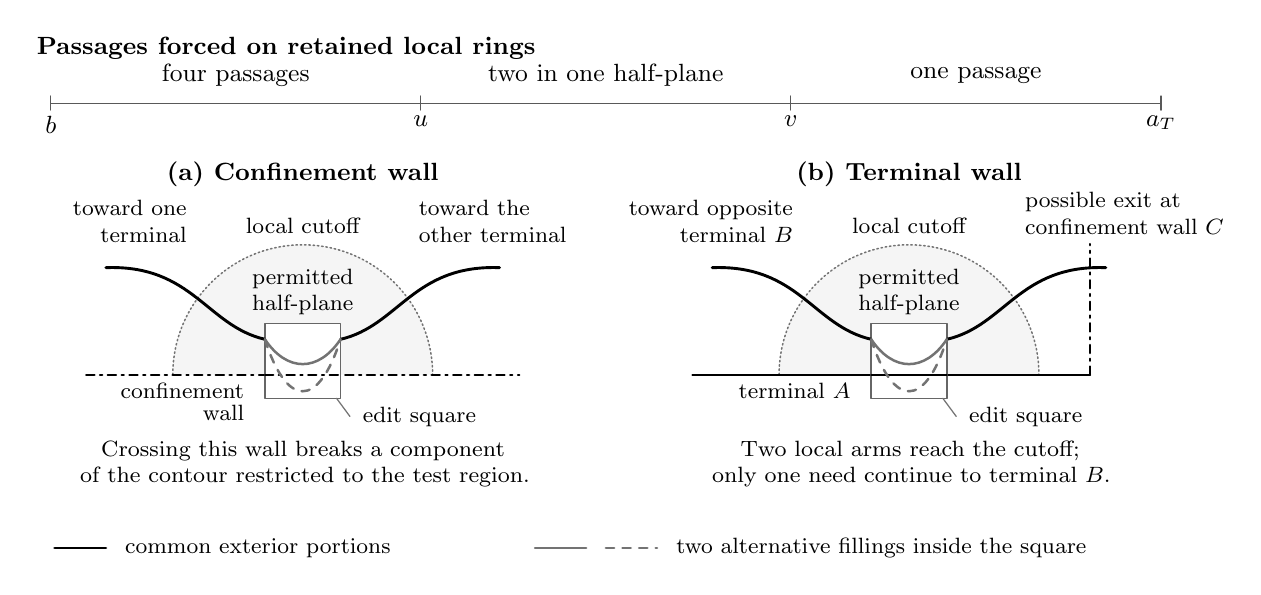
\begin{tikzpicture}[x=1cm,y=1cm,line cap=round,line join=round,
  every node/.style={font=\small},
  common/.style={black,line width=1.05pt},
  fillone/.style={black!55,line width=.9pt},
  filltwo/.style={black!55,line width=.9pt,dashed},
  cutoff/.style={black!55,line width=.55pt,densely dotted},
  confinement/.style={black,line width=.8pt,dash dot},
  terminal/.style={black,line width=.8pt}]

 \node[anchor=west,font=\small\bfseries] at (.15,6.6)
   {Passages forced on retained local rings};
 \draw[black!65] (.45,5.9)--(14.55,5.9);
 \foreach \x/\lab in {.45/b,5.15/u,9.85/v,14.55/a_T}{
   \draw[black!65] (\x,5.81)--(\x,5.99);
   \node[below,inner sep=2pt] at (\x,5.81) {$\lab$};
 }
 \node[align=center] at (2.8,6.25) {four passages};
 \node[align=center] at (7.5,6.25) {two in one half-plane};
 \node[align=center] at (12.2,6.25) {one passage};

 \begin{scope}[shift={(3.65,2.45)}]
  \node[font=\small\bfseries] at (0,2.55) {(a) Confinement wall};
  \fill[black!4] (-1.65,0) arc[start angle=180,end angle=0,radius=1.65]--cycle;
  \draw[cutoff] (-1.65,0) arc[start angle=180,end angle=0,radius=1.65];
  \node[font=\footnotesize] at (0,1.89) {local cutoff};
  \node[font=\footnotesize,align=center] at (0,1.05)
    {permitted\\half-plane};
  \draw[confinement] (-2.75,0)--(2.75,0);
  \node[anchor=east,font=\footnotesize] at (-.62,-.20) {confinement};
  \node[anchor=east,font=\footnotesize] at (-.62,-.48) {wall};
  \fill[white] (-.48,-.30) rectangle (.48,.65);
  \draw[black!60,line width=.55pt] (-.48,-.30) rectangle (.48,.65);
  \draw[confinement] (-.48,0)--(.48,0);
  \draw[common] (-2.5,1.36) .. controls (-1.4,1.4) and (-1.22,.62) .. (-.48,.45);
  \draw[common] (.48,.45) .. controls (1.22,.62) and (1.4,1.4) .. (2.5,1.36);
  \draw[fillone] (-.48,.45) .. controls (-.20,.03) and (.20,.03) .. (.48,.45);
  \draw[filltwo] (-.48,.45) .. controls (-.20,-.43) and (.20,-.43) .. (.48,.45);
  \node[font=\footnotesize,anchor=east,align=right] at (-1.35,1.95)
    {toward one\\terminal};
  \node[font=\footnotesize,anchor=west,align=left] at (1.35,1.95)
    {toward the\\other terminal};
  \draw[black!55,line width=.45pt] (.60,-.53)--(.43,-.30);
  \node[font=\footnotesize,anchor=west] at (.64,-.53) {edit square};
  \node[font=\footnotesize,align=center,text width=6.6cm] at (0,-1.13)
    {Crossing this wall breaks a component\\of the contour restricted to the test region.};
 \end{scope}

 \begin{scope}[shift={(11.35,2.45)}]
  \node[font=\small\bfseries] at (0,2.55) {(b) Terminal wall};
  \fill[black!4] (-1.65,0) arc[start angle=180,end angle=0,radius=1.65]--cycle;
  \draw[cutoff] (-1.65,0) arc[start angle=180,end angle=0,radius=1.65];
  \node[font=\footnotesize] at (0,1.89) {local cutoff};
  \node[font=\footnotesize,align=center] at (0,1.05)
    {permitted\\half-plane};
  \draw[terminal] (-2.75,0)--(2.30,0);
  \draw[confinement] (2.30,0)--(2.30,1.66);
  \node[anchor=east,font=\footnotesize] at (-.62,-.20) {terminal $A$};
  \fill[white] (-.48,-.30) rectangle (.48,.65);
  \draw[black!60,line width=.55pt] (-.48,-.30) rectangle (.48,.65);
  \draw[terminal] (-.48,0)--(.48,0);
  \draw[common] (-2.5,1.36) .. controls (-1.4,1.4) and (-1.22,.62) .. (-.48,.45);
  \draw[common] (.48,.45) .. controls (1.22,.62) and (1.4,1.4) .. (2.50,1.36);
  \draw[fillone] (-.48,.45) .. controls (-.20,.03) and (.20,.03) .. (.48,.45);
  \draw[filltwo] (-.48,.45) .. controls (-.20,-.43) and (.20,-.43) .. (.48,.45);
  \node[font=\footnotesize,anchor=east,align=right] at (-1.35,1.95)
    {toward opposite\\terminal $B$};
  \node[font=\footnotesize,anchor=west,align=left] at (1.35,2.05)
    {possible exit at\\confinement wall $C$};
  \draw[black!55,line width=.45pt] (.60,-.53)--(.43,-.30);
  \node[font=\footnotesize,anchor=west] at (.64,-.53) {edit square};
  \node[font=\footnotesize,align=center,text width=6.6cm] at (0,-1.13)
    {Two local arms reach the cutoff;\\only one need continue to terminal $B$.};
 \end{scope}

 \draw[common] (.5,.25)--(1.15,.25);
 \node[anchor=west,font=\footnotesize] at (1.27,.25) {common exterior portions};
 \draw[fillone] (6.6,.25)--(7.25,.25);
 \draw[filltwo] (7.5,.25)--(8.15,.25);
 \node[anchor=west,font=\footnotesize] at (8.27,.25) {two alternative fillings inside the square};
\end{tikzpicture}

\caption{Local geometry in Lemma~\ref{lem:stability-pivotal}.
The scale strip records the four-, two-, and one-passage regimes;
intervals may be empty, and rings near their endpoints are omitted
as in the lemma. Passages are counted by disjoint parameter intervals
and may lie on a single contour. The panels show the intermediate regime, with
the local cutoff below the next vertex and the other terminal.
Black contour portions agree outside the edit square; the two gray
fillings are alternatives. Crossing a confinement wall ends a
component restricted to the permitted region, whereas crossing a
terminal wall creates a terminal hit. In (b), one local arm may
later exit at the confinement wall~$C$, so the two local arms need
not form two full $A$--$B$ passages. The semicircular cutoffs are
schematic; the ring checks use the fixed crops and recenterings
specified in the lemma.}
\label{fig:pivotal-walls}
\end{figure}

\begin{proof}
Choose $a_T$ smaller than the separation of distinct nonincident
sides, the lengths of all sides, and the distances between the
disjoint terminal sets, with additional fixed reductions depending
on the finitely many vertex angles.  Then a ball below this scale
meets no test wall, just one straight wall, or walls incident to
one nearby vertex.  This choice is essential for a thin polygon:
distance to a vertex alone need not exclude a second, nonincident
side.  Capping at $a_T$ removes that difficulty.  Enlargement and
recentering cost only fixed factors for this test.

First work in a neighborhood meeting no test wall.  Cut the common
exterior contours at their intersections with the enlarged edit
square, making an arbitrarily small displacement of the cut to
avoid vertices.  Follow every exterior end to its first return to
the square or to the local outer cutoff.  An exterior connection
which reaches that cutoff supplies two long ends; short returns
can be contracted for this argument.  The number of long ends
is even.  If it is zero, the edit is screened within the cutoff.
If it is two, the interior filling, together with the short
exterior returns, must connect these same two ends in either
configuration.  It can add small closed curves but cannot change
their through connection or the two side colors seen outside the
cutoff.  Since there is no terminal in this neighborhood, these
small curves cannot create a terminal visit.  A changed passage
count therefore requires at least four long contour portions.
This argument is about cut parameter intervals, and allows all
four portions to come from one loop.

More explicitly, the filling together with short exterior returns
is a degree-two network whose only free ends are the long ends.
With two such ends it has one connecting path and terminal-free
cycles.  Restrict each resulting contour to the permitted test region,
breaking its parameter interval wherever it exits that region.  On each
remaining component record the successive inner and outer terminal
visits in parameter order, cyclically on a closed component, collapsing
consecutive visits of the same type.  The maximal
number of disjoint passages is the number of changes of terminal type
within these components.  A confinement-wall exit ends a component;
visits on opposite sides of such an exit are not paired.  Replacing
the terminal-free connecting path in the present wall-free neighborhood
preserves these sequences and their component endpoints.  This also
covers repeated visits by one contour and small terminal-free loops.

For a color-crossing test the same conclusion also follows by
juxtaposing a successful path and the blocking path of the
opposite color in the configuration where the test fails.  The
triangulation gives the exact crossing--blocking alternative.
Both paths must meet the edit square.  Outside it they supply
four alternating color continuations, whose intervening contours
give four long portions.  Cutting a band along a radial path
gives the identical argument for a circuit and its radial
blocker.

Next suppose that only one straight wall is present.  There are
two different wall roles for passage tests.  At a confinement
wall, a passage disrupted by the edit has a part on either side
of the disrupted portion leading back to the local cutoff in
the permitted half-plane; its terminal walls lie beyond that
cutoff.  These are the two required portions.  At a terminal
wall, stop every passage at its first terminal hit.  A portion
which hits this terminal before entering the edit neighborhood
is unchanged.  Among the remaining portions arriving from the
opposite terminal, a terminal hit can disappear only if the new
filling pairs its long end with another long end on the permitted
side.  Pairing with an end on the other side still crosses the
terminal wall and preserves a hit.  If there is only one long end
on the permitted side, neither pairing can remove the hit.
Consequently a changed terminal visit supplies two long portions
in the permitted half-plane.  A
hairpin tip moved across a terminal is covered by this case:
its two local arms supply the required half-plane portions.
In a confined test only one arm may continue all the way to the
opposite terminal, so the passage count need not change by two.

For a crossing and its blocker, at most the color arm directed
towards this single wall can terminate before the local cutoff.
The other three occur in alternating order on the permitted
side.  The two transitions between them give two disjoint
contour portions in that half-plane.  The circuit argument is
the same after the radial cut.  In each case start the
half-plane rings at a fixed multiple of the distance to the
wall and stop before the next vertex scale; the contours in
question stay on one consistent permitted side.  If the test
permits either side, taking the union of the two checks costs
at most a factor two per retained ring.

Above the vertex scale we retain only one contour portion.
For a crossing and blocker, two adjacent incident walls can
terminate two of the color continuations, but a transition
between the remaining colors persists towards the separated
terminal.  For a passage test, an affected passage still has
a portion towards its other terminal, at distance at least
$a_T$.  Equivalently, if no contour exits the local cutoff,
every change is confined to components which cannot connect
the separated terminal sets or alter a separating circuit.
Thus a pivotal change forces one passage up to $a_T$.

At every step the portions are cropped at the appropriate
first or last hits.  No positive-length interval is used
twice, even when a contour returns repeatedly to a wall.
The fixed-factor omissions accommodate the chosen cuts,
recentering, and the transition between the three geometric
regimes.  An $O(\delta)$ displacement of a wall is absorbed
by increasing the starting square and, for the half-plane
checks, translating its line outwards by $O(\delta)$.
\end{proof}

\subsection{A half-plane estimate under bulk conditions}

The pivotal-square lemma requires a bound $o(r/R)$ for two passages
constrained to one side of a bulk line.  We obtain it by counting
macroscopic subarcs, bounding the area of their near-support contacts,
and then separating off a four-passage alternative.
Propositions~\ref{prop:pure-four-passages} and~\ref{prop:pure-rsw}
give, for some $c>0$,
\begin{equation}
 \limsup_{\delta\downarrow0}\P_0(F_4(z,\theta;r,R))
       \leq C(r/R)^{2+c},
 \qquad
 \limsup_{\delta\downarrow0}\P_0(F_1(z,\theta;r,R))
       \leq C(r/R)^c.
 \label{eq:stability-pure-41}
\end{equation}
The ratios are fixed before the mesh limit.  Buffered comparisons
transfer these statements between the plane, a larger disk with plus
boundary, and bulk torus charts, with fixed multiplicative constants.
We next supply the estimate between them.  It concerns a geometric
half-plane inside a bulk chart, not a model with boundary conditions on
the straight line.

\begin{lemma}[Integrable numbers of macroscopic subarcs]
\label{lem:stability-counts}
Fix a compact region $K$ and a length $a>0$, in a bulk chart containing
a fixed $20a$-neighborhood of $K$.  There is a random finite list
$\mathcal L_\delta$ of compact contour parameter-subarcs, chosen without
reference to a test center or direction, with
$\sup_\delta\E|\mathcal L_\delta|<\infty$ for sufficiently fine meshes.
The list covers the following visits, with their contour multiplicities.
If a contour visits $x\in K$ and reaches distance $10a$ from $x$ in
both parameter directions, a member of the list contains that visit and
lies between the first such distant visit in each direction.  Subarcs
are retained only in a fixed enlargement of $K$.  The same assertion
holds for the limiting complete loop collection, with a list of finite
expected cardinality.  Fixed enlargements of the chart and fixed crops
of the excursion lengths only change the bound.
\end{lemma}

\begin{proof}
First consider a rectangle of fixed shape, with an unexamined buffer
around it.  Contour crosscuts between its horizontal sides, confined
between two vertical sides, are linearly ordered from left to right.
After cropping their ends, each crosscut has two colored side routes.
One obtains these routes by following the open spin regions next to
the interpolated contour and then following vertices in the
triangulation.  The two routes associated with one crosscut have
opposite signs.  Reading the routes in their planar order and retaining
successive sign changes produces an alternating list whose length is
at least a fixed fraction of the number of crosscuts.  Opposite signs
cannot meet.  Routes of the same sign separated by an opposite route
are disjoint as crossings.  The fixed end crop and side margins absorb
the interpolation distance.  Thus it suffices to bound the number of
ordered alternating spin crossings of a fixed rectangle.

Explore the leftmost crossing of a prescribed sign, if one exists.
The exploration examines only the sites on its left and the crossing
itself.  For example, reveal the vertices reachable from the examining
side before a crossing of that sign blocks the exploration; their
outer envelope gives the same leftmost path.  An alternative path
lying farther left somewhere is detectable on this examined side by
splicing at its first and last common vertices.  Consequently the
transcript leaves the spins to the right with the ordinary Ising
conditional law, and the only newly exposed spins facing that region
on the separating path have the prescribed sign.  Repeat for the
opposite sign in the remaining right region.  Previously examined
sites lie behind the most recent spanning path.

There is a uniform probability $c_0>0$, conditional on each successful
transcript, that no further opposite crossing can occur.  We construct
the blocking event in a deterministic rectangle, rather than asking RSW
for a crossing ending on the random exposed path.  For one fixed choice of proportions, take the counting slab to be
$[-1,1]\times[-2,2]$, and let $\Gamma$ be the exposed simple
color-$s$ crossing from its bottom to its top.  Use the central rectangle
$[-2,2]\times[-1,1]$ for a horizontal test, with end gates on
$x=-2$ and $x=2$, and surround it by the larger rectangle
$[-4,4]\times[-3/2,3/2]$.  Fixed changes of these proportions cover
the original rectangle shapes.

In the larger rectangle, fill the side to the left of $\Gamma$ by
color $s$, leave its right side free, and put color $-s$ on the outer
boundary.  The side is determined by the bottom-to-top crosscut in the
counting slab; its restriction to the central levels suffices, even
when it has bulges or crosses a horizontal level several times.
Nearest-neighbor conditional independence makes the filled left side
invisible from the right except through the color-$s$ path.  All
earlier revealed sites are screened by that path.  No sites to the
right of the counting slab have been examined, so the lateral extension
retains a free region past the right gate.  Thus, for increasing tests
when $s=+$, the actual remaining law dominates this right-side law;
putting the outer pins at minus only lowers it.  For $s=-$ the order
is reversed.

The filled comparison law in turn dominates, in the color-$s$ order,
the ordinary law in the same larger rectangle with all boundary spins
$-s$ and no interior pins.  In this last, deterministic law, a
color-$s$ horizontal crossing of the central test has probability at
least $c_0$ by Proposition~\ref{prop:pure-rsw}; its gates and test
collars are a positive distance from the outer pins.  Such a crossing
must meet $\Gamma$, since its gates lie on opposite sides of the
counting slab.  Its portion after the last meeting with $\Gamma$
connects the exposed path to the right gate.  It therefore blocks
another color-$-s$ vertical crossing confined to the slab.  This
suffix uses only the unexplored side, so the two monotone comparisons
prove the asserted conditional stopping probability.  The central
vertical crop leaves clearance from the endpoints of $\Gamma$;
lattice rounding is absorbed by the fixed margins.

The chance of continuing the alternating exploration after $m$
successful crossings is therefore at most $(1-c_0)^{m-1}$, with a
factor two for the initial color.  This gives uniformly bounded
moments of all orders for the number of contour crosscuts in a fixed
cropped rectangle.

Cover a fixed enlargement of $K$ by finitely many squares of diameter
much smaller than $a$.  Every departure by distance $a$ from one such
square contains a passage through one of finitely many buffered
rectangles; choose the first side through which an appropriate
enlargement is left.  Disjoint parameter intervals yield distinct
passages in this finite collection.  Their total number thus has
bounded expectation, indeed bounded moments.

Cut the contours at the boundary of an enlarged chart containing the
$20a$-neighborhood of $K$, and retain only components that meet $K$
and have diameter at least $10a$.
Subdivide each such parameter interval successively when its distance
from the last subdivision point first reaches $a$.  For a closed
component choose a root without reference to the later center or
direction and subdivide cyclically.  Retain every union of five consecutive
subdivision intervals whose middle interval meets $K$.  The interval
containing a qualifying visit is therefore the middle of one listed
union.  That union lies within distance less than $10a$ of the visit, after an absolute reduction of the
subdivision distance if needed.  It therefore lies between the two
distant visits in the statement.  The buffer from $K$ to the cutting
boundary ensures that these intervals exist on both sides of every
qualifying visit.  Endpoint remainders and cyclic intervals through a
root are included.  The rectangle count bounds the number of retained
intervals, including separate traversals of the same geometric region.
This constructs the required list without subdividing any part of a
contour far from the fixed chart.

Complete-resolution convergence from Theorem~\ref{thm:pure-cle},
with slightly relaxed rectangles, preserves every fixed finite
collection of these macroscopic passages.  Fatou's lemma transfers
the expectation bound to the limit.  Alternatively perform the same
successive subdivision on the limiting loops: uniform continuity
makes the list finite on each loop, and the relaxed passage counts
bound its expected length.  The construction lists no microscopic
loops unrelated to the excursions under consideration.
\end{proof}

\begin{lemma}[Area of near-support contacts]
\label{lem:stability-tangency}
Fix a bulk region and a positive excursion length.  For the pure
contours at mesh $\delta$, let $G_K(z,\theta,u)$ be the event that a contour subarc
comes within $C u$ of $z$, travels the fixed excursion length on both
sides of this visit, and throughout those two portions stays above
the line of direction $\theta$ through $z$ lowered by $CKu$.
For each fixed $K$,
\begin{equation}
 \limsup_{\delta\downarrow0}\P_0(G_K(z,\theta,u))=o_K(u),
 \label{eq:stability-tangency}
\end{equation}
as $u\downarrow0$ with $K$ fixed, uniformly over centers and directions
in a smaller bulk chart. Fixed crops or fixed changes of the constants
have the same conclusion.
\end{lemma}

\begin{proof}
Use a larger round disk with plus boundary as a reference and average
the center over the lattice translates of a small disk in its interior.
Translation invariance of the plane law and pure buffered density
comparison bound the plane probability at a specified center by
a constant times this averaged reference probability.  Off-lattice
centers are covered by an $O(\delta)$ relaxation of the distances.
This step uses only lattice translations.  Complete loop convergence
with relaxed distances then bounds its upper limit by the analogous
continuum event averaged over area.  Indeed every witnessing subarc
has a fixed positive diameter, so it belongs to the macroscopic part
of the loop ensemble; subsequential uniform parametrized convergence
preserves its closed near-visit and half-plane conditions after the
relaxation.  The reference disk and the
averaging disk are rotationally invariant.  We may therefore average
also over the direction in this continuum bound.  For directions or
centers varying with the mesh, take convergent subsequences and relax
the geometric inequalities before applying loop convergence.  This
gives the same uniform bound and does not assert rotational
invariance of the lattice.

Use Lemma~\ref{lem:stability-counts} with a subdivision length smaller
than one tenth of the fixed excursion length.  If the event occurs,
one member $C$ of its list contains the near visit and lies entirely
between the distant visits.  This list is independent of $z$ and
$\theta$.  Write $n_\theta$ and $t_\theta$ for the upward normal and
the unit tangent to the line, and put
\[
 m_C(\theta)=\min_{w\in C}n_\theta\cdot w,
 \quad
 C_{\theta,h}=\{w\in C:n_\theta\cdot w\leq m_C(\theta)+h\}.
\]
For almost every $\theta$ the support line of the compact convex hull
of $C$ has a unique contact point.  One elementary justification is
to use the support function of that convex hull: it is Lipschitz
on the circle and differentiable almost everywhere, and at a
differentiability direction the two extreme tangent coordinates of
the supporting face coincide.  Compactness then gives
\begin{equation}
 \operatorname{diam}\{t_\theta\cdot w:w\in C_{\theta,h}\}
       \longrightarrow0\qquad(h\downarrow0)
 \label{eq:stability-support-width}
\end{equation}
at each such direction.

If $C$ supplies a near visit, its height above its minimum at that
visit is at most $C_Ku$.  The normal coordinate of $z$ lies in an
interval of length $C_Ku$ about $m_C(\theta)$, and its tangent
coordinate lies within $Cu$ of the projection of $C_{\theta,C_Ku}$.
The area of the possible centers is therefore bounded by
\[
 C_Ku\left(\operatorname{diam}
          \{t_\theta\cdot w:w\in C_{\theta,C_Ku}\}+Cu\right).
\]
By \eqref{eq:stability-support-width} this is $o_K(u)$ for almost
every direction and is at most $C_Ku$ times a fixed chart diameter.
The expected number of arcs in the list is finite.  Dominated
convergence first over directions and then over that list proves
the averaged $o_K(u)$ bound.  The preceding buffered comparison and
rotational averaging yield \eqref{eq:stability-tangency}.
\end{proof}

\begin{proposition}[Two bulk passages confined to a half-plane]
\label{prop:pure-half-plane}
For the events in \eqref{eq:stability-checks}, in any buffered pure
bulk chart,
\begin{equation}
 \limsup_{\delta\downarrow0}\P_0(H_2(z,\theta;r,R))=o(r/R)
 \quad\text{as }r/R\downarrow0.
 \label{eq:stability-halfplane}
\end{equation}
The ratio is fixed before taking the mesh limit.  The assertion is
uniform in translations and rotations of the fixed geometry, and
continues to hold with fixed proportional crops.
\end{proposition}

\begin{proof}
Normalize $R=1$ and write $u=r/R$.  Select two confined passages.
If there are fewer than four unconstrained passages from radius
$u$ to radius $Ku$, they belong to the same loop and their inner
ends are joined inside radius $O(Ku)$.  To verify the statement
including multiplicities, first suppose that the selected passages
belong to different loops.  The complementary arc on each loop
supplies a second passage to $Ku$, giving four in total.  On a
single loop the two complementary arcs either both join an inner
end to an outer end, again giving four, or join inner to inner and
outer to outer.  In the latter case an excursion of the inner
connecting arc to $Ku$ supplies two further passages.  These may
share their outer hit, as allowed by our convention, and have
disjoint interiors.  Thus that excursion is excluded.

Concatenate the two confined passages and their inner connecting
arc.  This subarc has a near visit to $z$ and goes a fixed positive
distance on both sides, all above the original line lowered by
$CKu$.  Its probability is $o_K(u)$ by
Lemma~\ref{lem:stability-tangency}.  In the complementary case there
are four passages from $u$ to $Ku$, and the original confined
passages still give two confined passages from $C_0Ku$ to $1$.
Here $C_0$ is a fixed buffer constant.  Condition on the spins
outside radius $C_0Ku$.  Pure buffered comparison bounds the
conditional four-passage probability by $CK^{-2-c}$, uniformly in
those outside spins, by \eqref{eq:stability-pure-41}.

Let $p(u)$ be the mesh upper limit of the plane confined-passage
probability, with the uniform translation and direction convention
just described.  We have proved, for every sufficiently large fixed
$K$ and all sufficiently small $u$,
\begin{equation}
 p(u)\leq o_K(u)+CK^{-2-c}p(C_0Ku).
 \label{eq:stability-half-recursion}
\end{equation}
All constants associated with buffers and relaxed squares are fixed
before $K$ is enlarged.  Square and Euclidean radii differ by fixed
factors and give the same recursion after changing $C_0$.

For completeness, put $q(u)=p(u)/u$, $d=C_0K$, and
$\vartheta=CC_0K^{-1-c}$.  Fix $K$ so large that $\vartheta<1$.
Then $q(u)\leq e_K(u)+\vartheta q(du)$, where $e_K(u)\to0$.
Iterate until $d^mu$ first reaches a fixed small interval bounded
away from zero.  The terminal value is bounded because $p\leq1$,
and
\[
 q(u)\leq\sum_{j=0}^{m-1}\vartheta^j e_K(d^ju)
                 +\vartheta^m q(d^mu).
\]
This first gives boundedness of $q$ near zero.  Splitting the sum
at a fixed index, letting $u\downarrow0$, and then sending that
index to infinity gives $q(u)\to0$.  This proves the plane
assertion.  A final fixed buffered density comparison proves the
same assertion in the other pure bulk charts.
\end{proof}

The three pure probabilities now decay more strongly than their
respective location counts.  We need their consequence at one large
fixed annulus ratio, together with a product rule.  Neither step will
refer to the law of a configuration after it has been edited.

\subsection{Conditional ring products with independent marks}

At a given stage allow only marks of radius at most $b$.  A check on
an annulus is determined by the original spins in that annulus with
an $O(\delta)$ margin, and by the mark variables whose squares meet
this support.  It does not require the assigned spins outside this
support.  Denote its support by $A_j$ and this finite set of mark
indices by $\mathcal J_j$.

\begin{lemma}[Ring product bound]
\label{lem:stability-products}
There is a fixed constant $D$ with the following property.  Take
annular checks of the types \eqref{eq:stability-checks}, whose inner
radii exceed $C b$, and whose enlarged neighborhoods and
proportional inner and outer collars are disjoint.  More precisely,
after absorbing rotations and lattice margins, each check has a
collar $W_j$ of the form
\[
 S_{2R_j}(z_j,\theta_j)\setminus
       S_{r_j/2}(z_j,\theta_j),
\]
the other check supports lie outside $W_j$, and the sets
$\mathcal J_j$ are disjoint.  All collars lie in bulk torus charts.
For arbitrary independent mark probabilities at or below this
cutoff,
\begin{equation}
 \P\left(\bigcap_{j=1}^m T_j^+\right)
       \leq\prod_{j=1}^m D\P(T_j^+).
 \label{eq:stability-product}
\end{equation}
The constant $D$ depends on the fixed collar proportions and is
independent of the annular aspect ratios and the mark probabilities.
\end{lemma}

\begin{proof}
Condition on the original pure spins outside $W_j$ and on all marks
outside $\mathcal J_j$.  For each fixed value of the remaining
local marks, $T_j^+$ is simply an event of the pure spins on $A_j$.
Corollary~\ref{cor:pure-annular} gives the pointwise density bound
\begin{equation}
 \frac{d\mu_{0,N}(\sigma_{A_j}\mid\sigma_{W_j^c})}
      {d\mu_{0,N}(\sigma_{A_j})}\leq D.
 \label{eq:stability-ring-density}
\end{equation}
For clarity, the two parts of this comparison have fixed aspect:
the outer data are separated from $A_j$ by the collar outside
$S_{R_j}$, and the inner data by the collar inside $S_{r_j}$.
For the second comparison interchange the terminal sets in the
symmetric density-odds bound and regard the already fixed outer
data as common pins.  The two losses are independent of $R_j/r_j$.
No pins occur in the intervening free collars.

For rotated squares this comparison uses a fixed patch cover, as in
\cite[Corollary~2.6]{OpenAIStatic2026}, without rotating the lattice. Write $S_t=z+e^{i\theta}[-t,t]^2$.
Partition $A=S_R\setminus S_r$ into a bounded number of sets, each
contained in an axis-aligned square of radius $cR$, with $c>0$ fixed
and small. Each patch is separated from the changed data outside
$S_{2R}$ by a distance comparable to $R$, uniformly in $\theta$.
Factor the probability of the configuration on $A$ into successive
patch conditionals. Earlier patches and all inner data are common
pins, allowed by Proposition~\ref{prop:pure-buffered}, so the bounded
product costs a fixed factor. To change the inner data, partition
$S_{r/2}$ into a bounded number of patches of diameter $cr$ and change
them one at a time. Each is separated from the whole observed annulus
by distance comparable to $r$. Terminal symmetry gives the same bound,
with the remaining inner patches and the outer data common. These
two finite products are uniform in $R/r$ and $\theta$. Finally mix
the reference exterior data to obtain
\eqref{eq:stability-ring-density}. Fixed positive patch clearances
absorb lattice rounding.

The marks in $\mathcal J_j$ are independent of the conditioning
and of the original spins.  Integrating the pointwise bound over
their unchanged distribution gives
\[
 \P(T_j^+\mid\sigma_{W_j^c},M_{\mathcal J_j^c})
       \leq D\P(T_j^+).
\]
All other $T_i^+$ are measurable with respect to this conditioning.
Remove the factors one at a time to obtain
\eqref{eq:stability-product}.  This proof uses conditional laws
of $\sigma^0$ only.  In particular, it neither defines nor assumes
a conditional mixing estimate for an edited spin law.
\end{proof}

Choose a large fixed gap factor $G$.  In a range of available scales
retain rings of ratio $A$ whose successive inner radii have ratio
$GA$.  For $G$ large enough their collars and mark-index
neighborhoods satisfy Lemma~\ref{lem:stability-products}, including
the harmless recenterings of Lemma~\ref{lem:stability-pivotal}.
Fix also a monitoring constant $C_{\rm mon}$ larger than the
minimum-radius constant in Lemma~\ref{lem:stability-products}, enlarged
to allow the fixed crops and recenterings.  Around an inserted square
of radius $b$, begin each retained ring only when its inner radius
is at least $C_{\rm mon}b$.  Removing the preceding rings costs a
bounded number of rings, absorbed in the pivotal bound below.
Thus every retained check is among the checks monitored at that
activation stage; this is the scale closure used in the bootstrap.
First choose these constants and the density constant $D$.  Then choose $A$
large.  By \eqref{eq:stability-pure-41} and
Proposition~\ref{prop:pure-half-plane}, the three pure probabilities
at ratio $A$ can be made small enough that there are numbers
\begin{equation}
 p_4>2,\qquad p_h>1,\qquad p_1>0,
 \label{eq:stability-exponents}
\end{equation}
pure probability bounds $q_4,q_h,q_1$, and positive tolerances
$\tau_4,\tau_h,\tau_1$ such that
\begin{equation}
 D(q_i+\tau_i)<(GA)^{-p_i},\qquad i\in\{4,h,1\}.
 \label{eq:stability-slack}
\end{equation}
Increase $D$ first to include the possible two choices of
half-plane and any other fixed union of cropped checks.
The assertion for $h$ uses $q_h=o(A^{-1})$: after $G,D$ are fixed,
one can choose $A$ with $Dq_h<(GA)^{-1}$ with strict slack, and
then choose $p_h>1$ sufficiently close to one.  It does not require
a previously known half-plane power law.  The assertion for $4$
uses the strict exponent above two.  The assertion for $1$ uses
any positive one-passage exponent.

All these choices precede $s_0$.  At this fixed ratio, increase
$s_0$ so that the pure finite-mesh bounds $q_i$ hold uniformly
for every translated and rotated check with inner lattice radius
at least a fixed multiple of $Ls_0$, in the stated torus charts.
Such a threshold follows from the mesh-first pure estimates and
buffered comparison.  If uniformity in the frame failed, take
convergent directions and normalized offsets and use slightly
relaxed radii; their fixed margins give the same estimate.
This is a choice for three fixed shapes, rather than a uniform
claim over an increasing family of final polygonal tests.

Suppose for the moment that, with marks of radii at most $b$,
the probabilities of all needed possibility checks are at most
$q_i+\tau_i$.  Pack the retained rings in the three ranges of
Lemma~\ref{lem:stability-pivotal}.  Omitting only the bounded
number of transition rings, \eqref{eq:stability-product} and
\eqref{eq:stability-slack} give the following bound for the
possibility of a pivotal insertion of a square of radius $b$:
\begin{equation}
 C_T\left(\frac b u\right)^{p_4}
     \left(\frac u v\right)^{p_h}
     \left(\frac v{a_T}\right)^{p_1},
 \qquad b\leq u\leq v\leq a_T.
 \label{eq:stability-pivotal-probability}
\end{equation}
This probability does not include the mark of the inserted square.
If its addition first permits a different test value, choose a
witnessing assignment afterwards and revert the new square to
the old values, retaining all other assignments.  The two
configurations agree outside that square.  The required checks
outside it are therefore possible using the previous marks.
They are exactly the events to which the product bound applies.

\subsection{The area sum and the finite-size bootstrap}

\begin{lemma}[Counting potential insertion centers]
\label{lem:stability-area}
Assume the possibility bounds just used.  For a fixed polygonal
test $T$, the total contribution to its change probability from
all marks of level $k$ is at most
\begin{equation}
 C_T\epsilon 2^{-k}
       \min\{1,(\delta b_k^{\mathrm{lat}}/a_T)^{c_*}\},
 \label{eq:stability-level-bound}
\end{equation}
for a fixed $c_*>0$.  The assertion also holds during any spatially
nonuniform partial activation of that level.  For the three
fixed annular shapes the constant is uniform in their scale,
position, and rotation.
\end{lemma}

\begin{proof}
Use physical lengths and rescale $a_T$ to one.  Write
$b=\delta b_k^{\mathrm{lat}}/a_T$, and similarly rescale $u,v$.
Discard centers whose edit square does not meet the finite spin
support of $T$: their insertion cannot affect the test.
For $b\leq1$, divide the insertion centers into dyadic classes
with truncated distances comparable to $u,v$, where
$b\leq u\leq v\leq1$.  The area of one such class is at most
$C_Tuv$.  Indeed, when $v<1$ the relevant portion of an edge
has length $O_T(v)$ near a vertex, and its $u$-neighborhood
has area $O_T(uv)$.  When $v$ is comparable to one, the total
finite edge length is $O_T(1)$.  Centers far from the edges
belong to the capped class $u=v=1$.  Lower truncation at $b$
allows the same estimate after enlarging by one lattice cell,
so there are at most $C_Tuv/\delta_T^2$ centers, where
$\delta_T=\delta/a_T$ is the rescaled mesh.

The marking probability is bounded by
$C_L\epsilon2^{-k}\delta_T^2/b^2$.  Multiplication by the
number of centers and \eqref{eq:stability-pivotal-probability}
gives exactly
\begin{align}
 &C_T\epsilon2^{-k}\frac{uv}{b^2}
          (b/u)^{p_4}(u/v)^{p_h}v^{p_1}\nonumber\\
 &\hspace{15mm}=
 C_T\epsilon2^{-k}
          (b/u)^{p_4-2}(u/v)^{p_h-1}v^{p_1}.
 \label{eq:stability-area-factor}
\end{align}
This equality is where both location-count thresholds enter.
Let
$m=\min\{p_4-2,p_h-1,p_1\}>0$.  The three base ratios in the
last line belong to $(0,1]$ and their product is $b$.  Every
term is therefore at most $C_T\epsilon2^{-k}b^m$.
There are $O_T((1+\log(1/b))^2)$ dyadic pairs.  Absorbing
this factor into $b^{m/2}$ proves
\eqref{eq:stability-level-bound}, with $c_*=m/2$.

If $b\geq1$, the centers whose squares can affect the test
occupy area at most $C_Tb^2$.  The crude bound one on
pivotality, combined with the marking probability, gives
$C_T\epsilon2^{-k}$.  The same crude count covers $b$ within
a fixed factor of one.  Omitted transition rings at smaller
scales have already been absorbed into $C_T$ in
\eqref{eq:stability-pivotal-probability}.
The computation uses only upper bounds on individual mark
probabilities; partial activation can therefore be arbitrary
in space.  For a fixed annular shape the geometric constants
scale with its inner radius and are independent of its
location or orientation.
\end{proof}

\begin{proposition}[Uniform bootstrap of the three checks]
\label{prop:stability-bootstrap}
There is $\epsilon_*>0$, chosen from the three fixed annular
shapes and the fixed constants of the mark law, such that the
following holds on every sufficiently fine finite torus.
Activate the independent marks in order of increasing radius.
At a stage with maximum permitted radius $b$, every check of
ratio $A$ with inner radius at least $C_{\rm mon}b$, and with its
prescribed bulk collars, satisfies
\begin{equation}
 \P(T_i^+)\leq q_i+\tau_i,
 \qquad i\in\{4,h,1\}.
 \label{eq:stability-bootstrapped}
\end{equation}
This remains true throughout continuous, possibly spatially
nonuniform activation of marks of the current radius.
\end{proposition}

\begin{proof}
There are finitely many mark variables on the torus.  Activate
one level at a time, increasing its Bernoulli parameters
continuously from zero to their prescribed values.  Conditional
on the pure spins, the expectation of an increasing event of
these marks is a polynomial in their parameters.  Differentiating
in a parameter gives the probability that this index is pivotal
when its own mark is omitted.  Integration is the usual
finite-product interpolation identity and requires no monotonicity
in the spins.  For any collection of checks, even a continuum
of geometric frames, these expectations are uniformly Lipschitz
in the finitely many parameters: the sum of their absolute
parameter changes bounds the change of every event probability.
Thus their supremum is continuous as well.

Before any marks are activated, the estimates hold with strict
slack, by the choice of $s_0$.  At each stage monitor only
checks with inner radius at least $C_{\rm mon}$ times the current radius.
When the cutoff increases, some checks leave this collection.
They are not needed again: the rings used for a later insertion
start at a larger fixed multiple of that insertion's radius.
Conversely, any check still monitored at a given stage has
been monitored throughout all earlier stages.

Suppose there were a first failure of
\eqref{eq:stability-bootstrapped}.  Up to that stage all ring
possibility estimates used to control an insertion satisfy
\eqref{eq:stability-bootstrapped}; by continuity the same weak
bounds hold at the candidate first failure.  Each pivotal
insertion for any monitored check therefore satisfies
\eqref{eq:stability-pivotal-probability}.  Apply
Lemma~\ref{lem:stability-area} to that check, summing all
previous levels and the activated fraction of the current
level.  Since these checks are translates, rotations, and
dilates of only three fixed shapes, their total probability
increase is at most
\[
 C_{\mathrm{boot}}\epsilon\sum_{k\geq0}2^{-k}
       \leq2C_{\mathrm{boot}}\epsilon.
\]
Choose $\epsilon_*$ so that this is less than
$\frac12\min_i\tau_i$.  The first failure cannot occur.
The same estimate, being uniform over the frames, rules out
a failure occurring only as a supremum.  This proves the
bootstrap on each finite torus, before taking any limit.

The order of the choices is now explicit: fix the collars
and gap factor, choose $A$ and the tolerances, enlarge $s_0$,
and then choose $\epsilon_*$.  The finitely many universal
shapes determine $C_{\mathrm{boot}}$.  No later polygonal
test enters this choice.  The enlargement of $s_0$ is made
before the critical trajectory of
Theorem~\ref{thm:critical-trajectory} is constructed.
\end{proof}

\subsection{Vanishing for every fixed family}

\begin{proof}[Proof of Theorem~\ref{thm:bulk-stability}]
Fix one of the tests $T$ in the statement.  During increasing
activation of the marks, apply the finite-product interpolation
identity to $D_T$.  Its initial value is zero.  If a new mark
first makes $D_T=1$, choose two permitted assignments with
different test values and revert the newly permitted square
in a witnessing assignment.  Before its addition all
assignments gave one value.  We obtain two configurations
which differ only inside that square and change the test.
Lemma~\ref{lem:stability-pivotal} applies, and its required
outside checks are possibility events using the older marks.
Proposition~\ref{prop:stability-bootstrap} controls these
checks whenever the insertion is smaller than the test.
For larger insertions use the crude overlapping-square count
in Lemma~\ref{lem:stability-area}.  We conclude that
\begin{equation}
 \P(D_T=1)\leq C_T\epsilon
       \sum_{k\geq0}2^{-k}
       \min\left\{1,
          \left(\frac{\delta(Ls_k+O(1))}{a_T}\right)^{c_*}\right\}.
 \label{eq:stability-final-sum}
\end{equation}
Absent torus levels can be set to zero; the displayed
infinite sum is a convenient upper bound.  For every fixed
$k$, its factor in braces tends to zero with $\delta$.
Every summand is dominated by $2^{-k}$, whose sum is finite.
Dominated convergence therefore proves $\P(D_T=1)\to0$.
Equivalently first make the level tail small, and then refine
the mesh for the finitely many remaining levels.  This
argument keeps $\epsilon$ fixed; it does not require a new
smallness condition depending on $C_T$.

A union bound proves \eqref{eq:stability-main} for the fixed
finite family.  Under Proposition~\ref{prop:edit-coupling},
the perturbed configuration belongs to
$\mathcal C(\sigma^0,M)$ except with probability $o(1)$.
On the complement of that exceptional event and all $D_T$,
the entire test vector agrees with the pure vector.  Its
total-variation distance from the pure test-vector law tends
to zero.  The joint positivity and four-passage conclusions
follow respectively from Proposition~\ref{prop:pure-rsw}
and Proposition~\ref{prop:pure-four-passages}.
\end{proof}

We record the precise quantifiers in the upper-bound consequence.
For every fixed buffered square annulus of radii $r,R$,
\begin{equation}
 \limsup_{\delta\downarrow0}\P_{\mathrm{pert}}(F_4(z,\theta;r,R))
 \leq
 \limsup_{\delta\downarrow0}\P_{0,N}(F_4(z,\theta;r,R))
 \leq C(r/R)^{2+c}.
 \label{eq:stability-perturbed-four}
\end{equation}
Only after this mesh limit do we send $r/R$ to zero.  In particular,
for a fixed compact chart and fixed $R$, cover the possible centers
by an $r$-grid, enlarge the inner squares by a fixed factor, and
reduce the outer radius from $R$ to $R/2$.
The finite union for each fixed $r$ has at most $C r^{-2}$ members.
Applying \eqref{eq:stability-perturbed-four} to that finite family
and then sending $r\downarrow0$ gives
\begin{equation}
 \lim_{r\downarrow0}\limsup_{\delta\downarrow0}
 \P_{\mathrm{pert}}\bigl(\text{some center in the compact chart has
 four passages from }r\text{ to }R\bigr)=0.
 \label{eq:stability-compact-bottlenecks}
\end{equation}
Thus the family grows only after its own mesh limit has been taken.
Later fixed-buffer density comparisons will transfer this statement
from torus charts to the interior of the specified finite domains.

\section{An exact representation and comparison at boundary incidences}
\label{sec:comparison}

The bulk comparison of Section~\ref{sec:stability} concerns unconditioned
torus laws.  We now obtain the two tools needed to use it in a domain with
prescribed exterior spins.  The first orders spins across certain
\emph{strict} changes of boundary incidences.  The second compares all
interior spin events, pointwise in their densities, across a fixed free
buffer.  Neither tool requires positive association of the perturbed spin
law with arbitrary pins.

Throughout this section the inverse temperature is the value supplied by
Theorem~\ref{thm:critical-trajectory}.  We abbreviate the conditional spin
law of Lemma~\ref{lem:contour-spin} by
\(\nu_{\Omega,\lambda}^{\tau}
=\nu_{\Omega,\beta_c(J,U,\lambda),\lambda}^{\tau}\),
and write \(\mu_{\lambda,N}\) for the unconditioned law on a square torus
of side \(N\).  We take tori larger than the fixed interaction range and
than all the charts used below.  All thresholds in the local construction
depend only on the fixed interaction, not on a domain or its pins.

\subsection{Private auxiliary variables for a local factor}

Write \(K_0=\beta_0J\).  The spin weight can be expressed as
\begin{equation}
 \exp\left(K_0\sum_{uv}\sigma_u\sigma_v\right)
 \prod_{\alpha,x}F_\alpha(\sigma_{x+A_\alpha}),
 \qquad
 \max_\alpha\|F_\alpha-1\|_\infty\longrightarrow0
 \quad(\lambda\longrightarrow0).
 \label{eq:comparison-local-factors}
\end{equation}
Here the sum is over nearest-neighbor bonds, the index \(\alpha\) ranges
over a fixed finite list of finite supports, and \(x\) ranges over their
translates.  Every \(F_\alpha\) is positive.  Lemma~\ref{lem:contour-spin}
gives the factors coming from \(U\); the change
\(\beta_cJ-K_0\) is included as another bond factor.  Enlarging a support
does not change its factor.  Thus we may fix, for each \(\alpha\), a finite
nearest-neighbor tree \(T_\alpha\) whose vertex set contains \(A_\alpha\).
Singleton supports are allowed.

We use binary variables with values in \(\{-1,+1\}\).  A variable placed
on a bond will be called a \emph{bit}, to distinguish it from a physical
spin at a lattice vertex.  For a fixed integer \(M\), put \(M\) bits
\(b_{e,1},\ldots,b_{e,M}\) on every nearest-neighbor bond \(e=uv\).
Choose \(a>0\) so that
\begin{equation}
 \frac{M}{2}\log\cosh(2a)=K_0.
 \label{eq:comparison-bit-coupling}
\end{equation}
Then summing the bits in
\(\prod_{i=1}^M\exp(a(\sigma_u+\sigma_v)b_{e,i})\)
gives a spin-independent constant times
\(\exp(K_0\sigma_u\sigma_v)\).  In particular, every bit has a strictly
positive coupling to both ends of its bond.

The reason for using these variables is a strict distinction between
free spins and pins.  At the unperturbed vertex, summing the physical
spin gives $2\cosh(a\sum_i b_i)$, whereas fixing it to either sign
gives $\exp(\pm a\sum_i b_i)$.  In the first factor the conditional
odds of one bit increase with every other incident bit.  Its logarithmic
increments lie strictly between those of the minus and plus factors.
We will retain these finite-table inequalities under perturbation.
The construction below must therefore realize each local factor exactly
while changing every vertex table by a quantity tending to zero.

\begin{proposition}[Exact vertex representation]
\label{prop:bit-representation}
There is a finite choice of \(M\) such that, for all sufficiently small
\(\lvert\lambda\rvert\), positive functions
\[
 W_v\bigl(\sigma_v,b_{\mathcal B(v)}\bigr)
\]
represent the spin weight in \eqref{eq:comparison-local-factors} exactly,
up to a constant, as the spin marginal of \(\prod_v W_v\).
Here \(\mathcal B(v)\) is the set of the \(4M\) bits on bonds incident to
\(v\).  The same functions are used whether a physical spin is free or
pinned.  There are only finitely many local tables, and uniformly in
their entries
\begin{equation}
 W_v(\sigma,b)\longrightarrow
 W_v^0(\sigma,b):=\exp\left(a\sigma\sum_{i\in\mathcal B(v)}b_i\right)
 \quad\text{as }\lambda\longrightarrow0.
 \label{eq:comparison-table-limit}
\end{equation}
The representation applies to either sign of every sufficiently small
local perturbation.
\end{proposition}

\begin{proof}
We construct one factor on a tree \(T\), and then give different
constructions disjoint sets of bits.  For each complete spin pattern
\(t\in\{-1,+1\}^{V(T)}\), reserve two private bits on every edge of
\(T\), with the same coupling \(a\).  Conditional on all the physical
spins, these bits are independent in the unperturbed representation.
For the two bits on \(e=uv\), set \(D_e=b_{e,1}-b_{e,2}\).  Their
conditional moments are
\begin{equation}
 \E[D_e\mid\sigma]=0,\qquad
 q_e(\sigma_u,\sigma_v)
 :=\E[D_e^2\mid\sigma]
 =2\operatorname{sech}^2\bigl(a(\sigma_u+\sigma_v)\bigr)>0.
 \label{eq:comparison-duplicate-moments}
\end{equation}
At a vertex \(v\) of this private copy of \(T\), multiply its vertex
factor by
\begin{equation}
 1+c_{v,t}\,\one_{\{\sigma_v=t_v\}}
       \prod_{\substack{e\in E(T)\\e\ni v}}D_e.
 \label{eq:comparison-tree-correction}
\end{equation}
An empty product is one.  In the expansion of the product over vertices,
a chosen subset \(S\subseteq V(T)\) contributes one copy of \(D_e\) for
each end of \(e\) in \(S\).  If \(S\) is nonempty and proper, the
connectedness of \(T\) gives an edge with exactly one end in \(S\).
Its centered difference makes this term vanish upon summing the private
bits.  The only surviving terms are therefore the empty selection and
the full selection.  Their sum is
\begin{equation}
 1+\one_{\{\sigma_{V(T)}=t\}}
       \left(\prod_{v\in V(T)}c_{v,t}\right)
       \left(\prod_{uv\in E(T)}q_{uv}(t_u,t_v)\right).
 \label{eq:comparison-tree-identity}
\end{equation}
The same formula holds for a singleton tree, with an empty edge product.

For a target factor \(F\) on a subset of \(V(T)\), put
\[
 \varepsilon_t=F(t)-1,\qquad
 Q_t=\prod_{uv\in E(T)}q_{uv}(t_u,t_v)>0.
\]
Choose coefficients whose product is \(\varepsilon_t/Q_t\).
For example, if \(m=|V(T)|\), take absolute values
\(\lvert\varepsilon_t/Q_t\rvert^{1/m}\) at every vertex, place the sign
of \(\varepsilon_t\) at one prescribed vertex, and take all coefficients
zero when \(\varepsilon_t=0\).  Every coefficient tends to zero as
\(F\to1\), for either sign of \(\varepsilon_t\).
Equation~\eqref{eq:comparison-tree-identity} then realizes
\(1+\varepsilon_t\one_{\{\sigma_{V(T)}=t\}}\).
Use distinct private bits for different patterns.  Conditional
independence allows their contributions to be multiplied, and exactly
one pattern is active at a given physical spin configuration.  Hence
\[
 \prod_t\left(1+\varepsilon_t
                    \one_{\{\sigma_{V(T)}=t\}}\right)=F(\sigma).
\]

There are finitely many trees, finitely many patterns on each, and only
finitely many translated trees using a given bond.  First count these
uses, and choose \(M\) large enough to assign all their pairs of private
bits disjointly.  Unused bits retain their original factor.  This
allocation can be made translation covariant; its number is independent
of the size of the torus.  Choose \(a\) only after this finite allocation,
using \eqref{eq:comparison-bit-coupling}.
The product of all the factors
\eqref{eq:comparison-tree-correction} at \(v\), times \(W_v^0\), defines
\(W_v\).  Each \(D_e\) has absolute value at most two.  Since a vertex
belongs to only finitely many assigned trees, all correction factors are
positive when their coefficients are small enough.  Their tables then
converge uniformly to one, proving
\eqref{eq:comparison-table-limit}.  Summing all private channels, with
the physical spins fixed, proves the claimed exact identity.
\end{proof}

The construction need not be analytic in \(\lambda\): taking a root of
\(\lvert\varepsilon_t\rvert\) provides the required continuity.  The
analytic construction of the critical temperature was completed in
Section~\ref{sec:flow} before this representation was introduced.

\subsection{Strict local margins and their comparison consequence}

For a positive function \(H\) of bits, let
\[
 d_i\log H(b_{-i})
 =\log H(b_i=+1,b_{-i})-\log H(b_i=-1,b_{-i}).
\]
The function is \emph{log-supermodular} if every such increment is
nondecreasing in every other coordinate.  On a Boolean cube this is
equivalent to
\(H(b\wedge b')H(b\vee b')\ge H(b)H(b')\); it suffices to sum the
two-coordinate differences along coordinate paths.  A positive
probability mass with this property is also called MTP\(_2\).

Summing or fixing the spin at \(v\) gives respectively the factors
\[
 F_v(b)=W_v(+1,b)+W_v(-1,b),\qquad
 P_v^+(b)=W_v(+1,b),\qquad P_v^-(b)=W_v(-1,b).
\]
The conditional probability of a free physical spin being plus is
\[
 k_v(b)=\frac{W_v(+1,b)}{F_v(b)}.
\]
We distinguish these vertex factors from the conditional odds of a bit
in the entire measure, which also involve its other endpoint.

\begin{lemma}[Finite-table margins]
\label{lem:comparison-margins}
After decreasing the allowed interval of \(\lambda\), every free factor
\(F_v\) is strictly log-supermodular in each pair of distinct incident
bits, and every kernel \(k_v\) is strictly increasing in each incident
bit.  For every incident coordinate \(i\), moreover,
\begin{equation}
 \sup_b d_i\log P_v^-(b)
 <\inf_b d_i\log F_v(b)
 \le\sup_b d_i\log F_v(b)
 <\inf_b d_i\log P_v^+(b).
 \label{eq:comparison-strict-margins}
\end{equation}
The gaps are bounded below by a positive constant independent of the
volume and the pins.
\end{lemma}

\begin{proof}
At \(\lambda=0\), put \(H=a\sum_{j\ne i}b_j\).  Then
\[
 F_v^0(b)=2\cosh\left(a\sum_jb_j\right),\qquad
 d_i\log F_v^0=\log\cosh(H+a)-\log\cosh(H-a).
\]
Because \(-1<\tanh u<1\) for finite \(u\),
\begin{equation}
 -2a<d_i\log F_v^0<2a.
 \label{eq:comparison-base-pin-gaps}
\end{equation}
The increments of \(\log P_v^{-,0}\) and \(\log P_v^{+,0}\) are
exactly \(-2a\) and \(2a\).  For two distinct bits the mixed difference
of \(\log F_v^0\), writing \(H\) now for the contribution from all the
remaining bits, is
\[
 \log\cosh(H+2a)+\log\cosh(H-2a)-2\log\cosh H>0,
\]
by strict convexity.  Finally, the log odds of the free spin are
\(2a\sum_jb_j\), with increment \(4a>0\) in each bit.
There are only finitely many entries in these tables.  Their strictly
positive minimum gaps persist under the uniform positive perturbation
in \eqref{eq:comparison-table-limit}.  This proves all the assertions.
\end{proof}

The free factors therefore give an attractive law on bits when all
physical spins are free.  The factors of a pinned spin have not been
claimed attractive.  The strict inequalities
\eqref{eq:comparison-strict-margins} instead provide exactly the
cross-law comparisons needed below.  The comparison uses the
order-preserving Markov-chain argument underlying Holley's theorem
\citep[Theorem~(6)]{Holley1974}; here the strict incidence conditions
will order the single-bit conditional probabilities.

\begin{proposition}[Comparison at strict incidences]
\label{prop:strict-incidence}
Consider two laws formed from the same vertex factors \(W_v\), with
possibly different sets of pinned physical spins.  Label the laws lower
and upper.  Let \(V\) be a union of nearest-neighbor connected components
of their common free vertex set.  At each vertex outside \(V\) adjacent
to \(V\), require one of the following possibilities:
\begin{center}
\begin{tabular}{c|c}
lower law & upper law\\ \hline
free & pinned plus\\
pinned minus & free\\
pinned minus & pinned plus
\end{tabular}
\end{center}
Then there is a coupling in which all bits on bonds touching \(V\), and
all physical spins in \(V\), are lower than or equal to their upper-law
counterparts.  The assertion remains valid if arbitrary values of bits
on bonds not touching \(V\) have been conditioned on separately in the
two laws.  It consequently remains valid for arbitrary mixtures of
these exterior bit conditions.
\end{proposition}

\begin{proof}
Let \(\mathcal B(V)\) consist of all bits on bonds with at least one
endpoint in \(V\).  Condition in each law on all other bits.  After
summing every free physical spin, the conditional weight on
\(\mathcal B(V)\) is a product of vertex factors, restricted to the
conditioned values where necessary.  A vertex in \(V\) has every
incident bit in \(\mathcal B(V)\).  Its factor is the identical
attractive function \(F_v\) in the two laws.  Its contribution to the
conditional log odds of a bit is therefore ordered whenever the two
configurations of varying bits are ordered.

At an endpoint outside \(V\), the table in the statement and
\eqref{eq:comparison-strict-margins} order the two contributions to those
log odds, regardless of the values of all other incident bits.  This
last qualification allows both the separately conditioned bits and the
other varying bits at that endpoint to differ.  Adding the contributions
of the two endpoints orders the full single-bit conditional log odds.

Run single-bit heat-bath chains in the two finite state spaces, updating
the same coordinate and using the same uniform random number at each
step.  The ordered conditional probabilities preserve the coordinatewise
order.  Start from any ordered pair, and take a subsequential stationary
limit of the coupled chains.  Strict positivity makes each marginal
chain irreducible and gives its prescribed Gibbs measure as its unique
stationary law.  We have thus obtained an ordered coupling of the bits.

Conditional on all bits, the free physical spins are independent, with
the kernels \(k_v\).  At the vertices of \(V\) these kernels are the
same in both laws and are increasing by
Lemma~\ref{lem:comparison-margins}.  Another family of common uniform
random numbers gives the ordered physical spins.  Finally, the argument
worked for every pair of exterior bit configurations.  Integrating these
couplings against the two exterior distributions proves the mixture
assertion.
\end{proof}

Two equal-sign pins at a boundary vertex are deliberately absent from
the table.  Their perturbed factors need not have ordered increments
when their other incident bits differ.  In particular,
Proposition~\ref{prop:strict-incidence} does not imply unrestricted
boundary monotonicity or the FKG inequality for pinned physical spins.

\subsection{Stopped reveals and geometric shielding}

The spin paths used here lie in the fixed triangulation obtained by
adding the northwest--southeast diagonal to every elementary square.
On bulk faces this realizes the contour pairing in
Section~\ref{sec:introduction}.  Its edges do not cross, and it contains
every nearest-neighbor bond.  We record the precise role of a reveal, so
that conditioning on a crossing does not introduce an unexamined
assumption about a spatial Markov property of the spin interaction.

\begin{lemma}[Reveals with a monochromatic facing boundary]
\label{lem:comparison-stopped-reveal}
Suppose spins are queried one at a time, each next query and the stopping
decision being determined by the preceding queries and their answers.
Conditional on a complete transcript, the remaining law is exactly the
original law with the revealed spins pinned.  This remains true after
conditioning on any event determined by the transcript.

In a finite triangulated disk with a prescribed inner disk, one can
explore from its outer boundary for a shield of either color \(s\).
On success, no inner-disk spin has been queried, and every queried
neighbor of the remaining component containing that disk has color
\(s\).  A color-\(s\) circuit in a narrower annular band separating the
two disks guarantees success.  All queried sites are on the exterior
side of that circuit or on the circuit itself.

The corresponding exploration in a triangulated topological rectangle,
from one side toward the opposite side, determines whether there is a
color-\(s\) crossing between the other two sides.  On success its facing
boundary contains such a crossing, and the exploration queries no spins
strictly beyond it toward the opposite side.  If that crossing extends
past the ends of a comparison region, every nearest-neighbor incidence
from the region across the explored side meets a pin of color \(s\).
\end{lemma}

\begin{proof}
Fix a deterministic query order to resolve all choices.  A transcript
lists queried vertices \(v_1,\ldots,v_m\) and their values
\(s_1,\ldots,s_m\).  Any configuration agreeing with these values causes
the same successive choices and the same stopping decision, by induction
on the number of queries.  Thus the transcript event is the cylinder
\(\{\sigma_{v_i}=s_i:1\le i\le m\}\).  Conditioning on a
transcript-measurable event adds nothing once a compatible transcript
has been specified.  Independent exploration randomness, if used, can
first be conditioned on and then averaged out.

For the annular construction, query the outer graph boundary.  Keep a
queue of all revealed vertices of color \(-s\), and query every
previously unqueried triangulation-neighbor of a queued vertex before
removing that vertex from the queue.  Newly discovered vertices of color
\(-s\) join the queue; vertices of color \(s\) do not.  Declare failure
just before a query would enter the protected inner disk.  Declare
success when the queue has been exhausted.  This is a finite adaptive
procedure of the kind just considered.

On success let \(V\) be the unqueried nearest-neighbor component
containing the inner disk, or the union of such components if the chosen
inner set has more than one component.  An unqueried nearest neighbor
of \(V\) belongs to \(V\).  A queried neighbor cannot have color \(-s\),
since every neighbor of such a vertex was queried before its queue entry
was removed.  Hence every boundary incidence of \(V\) meets a revealed
\(s\) vertex.  If a color-\(s\) circuit separates the protected disk from
the outer boundary, every queued vertex has a color-\(-s\) path to the
outer boundary and so lies outside the circuit.  A further queried
neighbor cannot lie strictly inside: the edge to it would cross the
circuit without meeting a circuit vertex.  Planarity forbids this, and
expansion stops at vertices of the circuit because they have color
\(s\).  The positive separation of the narrower band from the protected
disk proves the asserted implication from a circuit to success.

For a topological rectangle, seed the exploration on the inspecting
side and expand color \(-s\) within the rectangle.  A color-\(-s\) path
reaching the opposite side certifies failure.  Otherwise the boundary
of the reached color-\(-s\) set facing that side gives a color-\(s\)
crossing between the two end sides.  To check this finite planar
assertion directly, join the reached components by a thin deterministic
strip immediately outside the inspecting side.  Trace the boundary of
a small polygonal neighborhood of this connected set on the side facing
the opposite boundary.  Since the reached set does not meet that
boundary, this trace has a component running between the two end sides.
Every graph vertex encountered just beyond the reached set was queried
and has color \(s\), because otherwise it would have been added to the
queue.  As the trace passes through a triangular face, consecutive such
vertices coincide or are joined by the remaining edge of that face.
They consequently give a walk of color \(s\) between the end sides.
Erasing closed subwalks gives a simple crossing.  Conversely a crossing
between the end sides blocks any opposite-color path between the
inspecting and opposite sides, since the two planar paths would have
to share a vertex.
Boundary arcs may be separated at their corners by one lattice step;
the prescribed buffered gates allow this harmless choice of finite
rectangle convention.  Thus the existence of the desired crossing is
determined by the transcript, and on success no queries pass strictly
beyond its facing boundary.  In applying this construction, the two end
gates lie past the comparison region, so a nearest-neighbor path cannot
go around a gate within that region.

Finally, a nearest-neighbor bond cannot cross a simple path or circuit
of the triangulation in the interior of an edge.  If its ends lie on
opposite sides, it must meet a path vertex.  This proves the incidence
assertion even when the separating path uses diagonal steps.
\end{proof}

Only the facing pins enter Proposition~\ref{prop:strict-incidence}.
Examined spins on the other side of a shield may have arbitrary signs,
and all of them remain part of the conditional law.  Likewise, when a
crossing test uses vertices outside one of its two comparison domains,
those vertices may be filled virtually by the extremal color for the
purpose of testing the increasing or decreasing event.  Such a filling
does not change any physical pin or any interaction.  The comparison
applies to the common free vertices after its incidence hypotheses have
been checked.

\subsection{From an extreme odds ratio to all interior densities}

Our final comparison will cut the auxiliary-bit graph along a square
inside the free buffer.  Conditional on all bit channels crossing that
cut, the interior law is the same in the domain and on the torus; the
exterior data change only the mixing law on the cut.  We must therefore
bound how much any two cut assignments can change the interior density.

For the bits of the \emph{unconditioned} torus, MTP\(_2\) reduces this
task to a single extreme odds ratio.  Two nested monochromatic shields
will bound that ratio using the incidence comparison and the circuit
probabilities from Section~\ref{sec:stability}.  We begin with the finite
algebraic reduction.  The four-difference identity below is the one used
in Lemma~2.1,
``Extreme rectangles in a ferromagnetic marginal'', in Section~2 of
\cite{OpenAIStatic2026}; its proof applies to any positive MTP\(_2\) mass.

\begin{lemma}[Rectangles of an MTP\(_2\) mass]
\label{lem:comparison-rectangles}
Let \(p(i,j)>0\) be an MTP\(_2\) probability mass on two disjoint finite
sets of binary coordinates \(I,J\).  Let \(i_-,i_+,j_-,j_+\) denote their
constant minus and plus configurations, set \(f=\log p\), and put
\begin{equation}
 \Lambda=f(i_+,j_+)+f(i_-,j_-)
              -f(i_+,j_-)-f(i_-,j_+)\ge0.
 \label{eq:comparison-extreme-ratio}
\end{equation}
Then, for arbitrary configurations \(a,a'\) on \(I\) and \(b,b'\) on
\(J\),
\begin{equation}
 \bigl|f(a,b)+f(a',b')-f(a,b')-f(a',b)\bigr|\le\Lambda.
 \label{eq:comparison-all-rectangles}
\end{equation}
Consequently every two conditional laws of \(I\) given \(J\), and every
two mixtures of those conditional laws, have pointwise density ratio
between \(e^{-\Lambda}\) and \(e^{\Lambda}\).
\end{lemma}

\begin{proof}
For \(u\le v\) and \(s\le t\), define
\[
 \Delta(u,v;s,t)=f(u,s)+f(v,t)-f(u,t)-f(v,s)\ge0.
\]
Writing \(D=f(a,b)+f(a',b')-f(a,b')-f(a',b)\), expansion gives the exact
identity
\begin{align*}
 \Lambda-D={}&\Delta(i_-,a';j_-,b)
             +\Delta(a,i_+;b',j_+)\\
             &+\Delta(a',i_+;j_-,b')
             +\Delta(i_-,a;b,j_+).
\end{align*}
Every term is nonnegative; no order between \(a,a'\), or between
\(b,b'\), is required.  Interchanging \(b,b'\) proves the other bound.

If \(q_b,q_{b'}\) are the two conditional masses on \(I\),
\eqref{eq:comparison-all-rectangles} says that
\(\log(q_b/q_{b'})\) has oscillation at most \(\Lambda\).  Its density
ratio has mean one under \(q_{b'}\), so its minimum is at most one and
its maximum is at least one.  Both bounds in the statement follow.
They persist after taking arbitrary mixtures in either law.
\end{proof}

We will also use preservation of MTP\(_2\) under marginalization.  Here
is a short proof in the finite setting at hand.  Sum one binary
coordinate \(z\) out of a positive MTP\(_2\) mass \(h\), and check the
increment ratio in another coordinate \(i\).  That ratio for the summed
mass is the conditional average, under \(h\) with \(i=-1\), of
\[
 r(z,y)=\frac{h(i=+1,z,y)}{h(i=-1,z,y)},
\]
where \(y\) denotes the other coordinates.  MTP\(_2\) makes \(r\)
nondecreasing in \(z\) and in every coordinate of \(y\).  The
conditional probability of \(z=+1\), with \(i=-1\), also increases when
one of those coordinates of \(y\) increases, by the corresponding
two-coordinate inequality for \(h\).  Thus the averaged ratio
increases.  This verifies each two-coordinate square for the marginal.
Iterating proves the assertion.  In particular, summing the physical
spins from the unconditioned representation gives the bit mass
\(\prod_vF_v\), which is MTP\(_2\), and any marginal of this bit mass
is MTP\(_2\) as well.

\begin{proposition}[Interior comparison across a fixed buffer]
\label{prop:interior-density}
Fix a square \(Q\) and a larger square \(\widetilde Q\), with
\(\overline Q\subset\operatorname{int}\widetilde Q\), in a fixed
physical torus chart.  Take lattice mesh \(\delta\downarrow0\), with
torus side \(N\) chosen so that this chart has a fixed macroscopic
buffer from its translates.  Suppose every lattice vertex in
\(\widetilde Q\) is free in a domain spin law
\(\nu_{\Omega,\lambda}^{\tau}\).  For all sufficiently small mesh there
is a constant \(C<\infty\), depending on the two fixed squares and the
chart but not on \(\Omega,\tau\), or the mesh, such that
\begin{equation}
 C^{-1}\le
 \frac{\nu_{\Omega,\lambda}^{\tau}(\sigma_{Q\cap\delta\Z^2}=\eta)}
      {\mu_{\lambda,N}(\sigma_{Q\cap\delta\Z^2}=\eta)}
 \le C
 \quad\text{for every spin configuration }\eta.
 \label{eq:comparison-interior-density}
\end{equation}
The same bounds hold for every event determined by these spins.
The exterior pins may be arbitrary, including those induced by any
admissible exterior contour configuration.
\end{proposition}

\begin{proof}
All sets in this proof are chosen in physical coordinates before the
mesh tends to zero.  We identify a lattice vertex with its rescaled
position when using \(Q\) and \(\widetilde Q\).  Let \(I\) contain all
bits incident to the vertices of \(Q\).  Choose two surrounding square
annular bands \(A_1,A_2\), with \(A_1\) inside \(A_2\), and then a
square cut outside \(A_2\), all within \(\widetilde Q\).  Leave positive
distances between successive objects.  The inner protected disk for an
exploration in \(A_1\) contains the endpoints of every bit in \(I\);
the inner protected disk for an exploration in \(A_2\) contains all of
\(A_1\).  Choose slightly wider exploration bands around \(A_1,A_2\),
still disjoint and separated from the cut.  A circuit in the original,
narrower band then implies exploration success by
Lemma~\ref{lem:comparison-stopped-reveal}.

More precisely, take a lattice square vertex set \(S\) containing both
exploration bands, with its boundary separated from them, and let \(J\)
be \emph{all} bit channels on the
nearest-neighbor bonds with one endpoint in \(S\) and the other outside.
We require \(I\) to lie strictly inside this cut.  Let
\(\mathcal B_{\mathrm{int}}(S)\) be the bits on bonds with both endpoints
in \(S\).  Every physical vertex in \(S\) is free.  Once \(J=j\) is
fixed, the conditional mass of the inside spins and bits is
\[
 K_S(\sigma_S,b_{\mathcal B_{\mathrm{int}}(S)}\mid j)
 =\frac1{Z_S(j)}\prod_{v\in S}W_v(\sigma_v,b_{\mathcal B(v)}),
 \qquad b_J=j.
\]
Every bit incident to a vertex of \(S\) is either an interior bit or
belongs to \(J\); all remaining vertex factors lie outside \(S\).
This proves the factorization and shows that \(K_S\) is identical in
the domain and torus laws.  In particular, their inside-bit marginals
can differ only through their mixing distribution on \(j\).
The representation is the same for all the laws by
Proposition~\ref{prop:bit-representation}; exterior pins in the spin
model are retained exactly by Lemma~\ref{lem:contour-spin}.

Let \(\widehat\mu\) denote the joint torus law of spins and bits, and
write \(\widehat\mu_j=\widehat\mu(\,\cdot\mid J=j)\).  For a sign
\(s\), let \(C_r^s\) be the fixed spin test of a color-\(s\) circuit in
\(A_r\), and let \(E_r^s\) be success of the exploration with that
color in its wider band.  These are different events.  The geometric
implication is
\begin{equation}
 C_r^s\subseteq E_r^s.
 \label{eq:comparison-circuit-success}
\end{equation}
Only the fixed tests \(C_r^s\) are used as inputs to bulk stability.
By Theorem~\ref{thm:bulk-stability} and the pure simultaneous
signed-circuit positivity of Proposition~\ref{prop:pure-rsw}, for all
sufficiently fine meshes
\begin{equation}
 \widehat\mu(C_1^+\cap C_2^-)
 \ge c,\qquad
 \widehat\mu(C_1^-\cap C_2^+)\ge c
 \label{eq:comparison-two-circuit-positivity}
\end{equation}
for a fixed \(c>0\).  We may take \(c\le1\).

We first show that, for \emph{every} cut configuration \(j\),
\begin{equation}
 \widehat\mu_j(C_1^+)\ge c,\qquad
 \widehat\mu_j(C_1^-)\ge c.
 \label{eq:comparison-circuits-all-cuts}
\end{equation}
Condition the unconditioned torus experiment on \(E_2^-\), and then on
a successful complete exploration transcript.  All physical spins of
\(A_1\) remain free.  Let \(V\) be the unqueried nearest-neighbor
component containing the protected inner disk, and hence all of \(A_1\).
It is a component of the common free set in the revealed experiment
and in \(\widehat\mu_j\).  Every neighbor outside \(V\) is a revealed
minus spin in the first experiment and a free spin in the second.
The queried outer boundary of the exploration separates \(V\) from
the cut, so no bit of \(J\) touches \(V\).  The minus-pin/free case of Proposition~\ref{prop:strict-incidence} orders
the conditional experiment below \(\widehat\mu_j\) on the spins of
\(A_1\).  Arbitrary further exterior bit conditions are allowed by that
proposition.  Average over the successful transcripts.  Since
\(C_1^+\) is increasing, this gives
\begin{align*}
 \widehat\mu_j(C_1^+)
 &\ge \widehat\mu(C_1^+\mid E_2^-)\\
 &=\frac{\widehat\mu(C_1^+\cap E_2^-)}
          {\widehat\mu(E_2^-)}
 \ge \widehat\mu(C_1^+\cap C_2^-)\ge c.
\end{align*}
The denominator is positive by
\eqref{eq:comparison-two-circuit-positivity}.  Interchanging the colors
and applying the comparison to the decreasing event \(C_1^-\) proves
the second inequality.  This step uses no monotonicity in the cut
configuration \(j\).

Now take the two extreme cut configurations \(j_-,j_+\), and denote the
corresponding laws by \(\widehat\mu_-\) and \(\widehat\mu_+\).
Under \(\widehat\mu_-\), the event \(E_1^+\) has probability at least
\(c\), by \eqref{eq:comparison-circuits-all-cuts} and
\eqref{eq:comparison-circuit-success}.  Conditional on any successful
transcript, the component containing all endpoints of \(I\) has facing
plus pins.  Compare it to \(\widehat\mu_+\) before any reveal.  The
plus-pin/free case of Proposition~\ref{prop:strict-incidence} makes
the former law larger on the bits \(I\).  The cut bits are outside the
comparison component in both experiments.  The increasing event
\(\{I=i_+\}\) therefore satisfies
\begin{equation}
 \widehat\mu_-(I=i_+)\ge
 \widehat\mu_-(E_1^+)\widehat\mu_+(I=i_+)
 \ge c\,\widehat\mu_+(I=i_+).
 \label{eq:comparison-plus-extreme}
\end{equation}
The opposite construction, starting from \(\widehat\mu_+\) and
revealing a minus shield, gives
\begin{equation}
 \widehat\mu_+(I=i_-)\ge
 c\,\widehat\mu_-(I=i_-).
 \label{eq:comparison-minus-extreme}
\end{equation}
These inequalities compare possibly very small probabilities; they do
not require a lower bound for either all-equal configuration on \(I\).

The joint torus bit marginal \(p(I,J)\) is positive and MTP\(_2\), by
Lemma~\ref{lem:comparison-margins} and marginalization as proved above.
Its extreme ratio satisfies
\[
 e^{\Lambda}
 =\frac{\widehat\mu_+(I=i_+)\widehat\mu_-(I=i_-)}
        {\widehat\mu_-(I=i_+)\widehat\mu_+(I=i_-)}
 \le c^{-2},
\]
by \eqref{eq:comparison-plus-extreme} and
\eqref{eq:comparison-minus-extreme}.  Apply
Lemma~\ref{lem:comparison-rectangles}.  It bounds the density ratio of
every two mixtures of the laws of \(I\) given \(J\) between \(c^2\)
and \(c^{-2}\).  One mixture is the torus law, and the other is the
domain law, by the exact cut factorization.

Finally, conditional on \(I\), the physical spins in \(Q\) have the
same product of Bernoulli kernels with plus probabilities \(k_v(I)\)
in both laws.  Integrating the pointwise bit-density inequalities
against this positive kernel gives
\eqref{eq:comparison-interior-density}, with \(C=c^{-2}\).
Summation gives the event version.  Every geometric separation was
fixed before taking the fine-mesh threshold, so the constant is
independent of the domain and its exterior pins.
\end{proof}

The buffer in Proposition~\ref{prop:interior-density} stays fixed when a
smaller test box shrinks inside \(Q\).  Consequently its constant can
be used for all boxes in a fine grid inside a compact chart.  Combining
it with the torus four-passage estimate of
Theorem~\ref{thm:bulk-stability} and
Proposition~\ref{prop:pure-four-passages} gives the compact-chart
bottleneck bound used in Section~\ref{sec:curves}.  That section gives
the grid argument with the order of the mesh and radius limits explicit.

\section{Signed boundary barriers and convergence of the full curve}
\label{sec:curves}

We now pass from the torus laws to the domains and exterior contours in
Theorem~\ref{thm:main}.  Theorem~\ref{thm:bulk-stability} compares finite
vectors of polygonal spin tests in the pure and perturbed tori.
Proposition~\ref{prop:strict-incidence} transfers colored crossings from
those tori to the target domain, after suitable boundary paths have been
revealed.  These crossings will place the target trace between two pure
comparison chords with the same limiting $\SLE_3$ law.

Identifying a trace does not determine its traversal order.  We use the
other output of Section~\ref{sec:comparison}, the fixed-buffer density
bound in Proposition~\ref{prop:interior-density}, to transfer the bulk
four-passage estimate to target interior events.  It rules out reverse
travel of positive diameter along the limiting chord and gives the
oriented curve metric~\eqref{eq:curve-metric}.  Thus density comparison
controls exceptional events; the colored-barrier argument identifies the
limiting law.

Fix a permitted $J,U$, and choose the perturbation interval small enough
for Theorem~\ref{thm:critical-trajectory}, Theorem~\ref{thm:bulk-stability},
and Proposition~\ref{prop:strict-incidence}.  No further reduction depending
on a domain will be made.  Throughout this section the perturbed model is
at $\beta_c(J,U,\lambda)$, and $\mu_{\lambda,N}$ denotes its torus spin
law.  The pure torus law is $\mu_{0,N}$.  Write
\[
 D_n=\delta_n D_{\Omega_n},\qquad
 \gamma_n=\delta_n\gamma(P_n).
\]
By Lemma~\ref{lem:contour-spin}, its spin law is the conditional law
$\nu_{\Omega_n,\beta_c,\lambda}^{\tau_n}$ with the actual exterior
configuration $\tau_n$ induced by $P_{o,n}$.  We keep $\gamma_n$ as the
prescribed resolution of $P_n$ and its two half-stubs.  Spin paths and
bulk passage tests use the fixed triangulation of
Section~\ref{sec:stability}.  In a bulk face, triangular interpolation
and the prescribed contour have the same connections and differ by
$O(\delta_n)$ with their traversal order preserved.

At the boundary one must distinguish the prescribed interface from the
zero set obtained by interpolating the entire exterior spin field.
Exterior-only disagreement edges can enter a boundary face and change
its full-plane connections.  We will instead redraw the target locally
beside the signed strips, using the geometric filling proved in
Lemma~\ref{lem:curves-local-barrier}.  This changes its drawing by
$O(\delta_n)$ and leaves the conditional spin law with exterior
$\tau_n$ intact.

\subsection{Fixed displaced domains and their boundary incidences}

Let $I_+$ and $I_-$ be the two open arcs of $\partial D$ carrying the plus
and minus exterior nearest neighbors.  There are only two choices.  It
suffices to treat a subsequence on which this choice is fixed.  Choose a
Jordan--Schoenflies homeomorphism $\Psi$ of the plane
\cite[Section~1 and Section~2(A), p.~860]{Cairns1951} such that
\[
 D=\Psi(\{\rho<1\}),\quad
 a=\Psi(1),\quad b=\Psi(-1),\quad
 I_+=\Psi(\{e^{i\theta}:0<\theta<\pi\}).
\]
Only the topology of these coordinates is used.  All spin tests will be
fixed polygonal tests in the original Euclidean coordinates.

We first construct a domain favoring minus, from which plus crossings
can be transferred to the target.  Move its plus boundary outward and
its minus boundary inward.  A minus corridor will screen the target's
minus arc, while a disjoint plus corridor will screen the comparison
domain's plus arc.  Conditioning a torus on both crossings then permits
the two strict-incidence comparisons.  The caps must extend beyond the
boundaries they screen, so that a common free component cannot go
around them.

For an explicit construction, take $0<h<\pi/30$, also small enough that
$3h<1/2$, and let $R_h$ be the continuous periodic
function which is $1+3h$ on $[4h,\pi-4h]$, is $1-3h$ outside
$(3h,\pi-3h)$, and is affine on the two remaining transition intervals.
The preliminary comparison domain is
\begin{equation}
 A_h^{\mathrm{top}}
 =\Psi\bigl(\{\rho e^{i\theta}:0\leq\rho<R_h(\theta)\}\bigr).
 \label{eq:curves-displaced-domain}
\end{equation}
Its marked points have angles $6h$ and $\pi-6h$, on the enlarged boundary.
The arc between them through $\theta=\pi/2$ is plus; the rest is minus.

Two disjoint topological rectangles implement the comparisons.  The
center of the minus rectangle $C_h^-$ follows $\rho=1-h$ along the long
angular interval $[\pi-h,2\pi+h]$.  At its two ends it bends radially
outward near angles $\pi-h$ and $h$, crosses $\rho=1$, and ends at gates
with $\rho>1+h$.  It is wholly outside $\overline{A_h^{\mathrm{top}}}$.
The center of the plus rectangle $C_h^+$ follows $\rho=1+h$ from angle
$5h$ to angle $\pi-5h$.  Its ends bend outward at those angles, cross
$\rho=1+3h$ on the minus part of $\partial A_h^{\mathrm{top}}$, and end
at gates with $\rho>1+4h$.  This rectangle is wholly outside $\overline D$.
Use sufficiently small positive widths.  Include slightly larger
rectangles on their radially exterior sides as the scopes in which a
crossing will be revealed.  The end caps of these larger rectangles still
cross, and extend beyond, the boundary being cut.  Compactness and the
strict inequalities just specified allow the widths to be chosen so that
\begin{equation}
 \overline{\operatorname{scope}(C_h^-)}\cap\overline{A_h^{\mathrm{top}}}
 =\varnothing,\qquad
 \overline{\operatorname{scope}(C_h^+)}\cap\overline D=\varnothing,
 \label{eq:curves-scope-clearances}
\end{equation}
and the two scopes are disjoint.  A lengthwise minus crossing cuts the
minus boundary of $D$ off from the center.  A lengthwise plus crossing
cuts the plus boundary of $A_h^{\mathrm{top}}$ off from the center.
Figure~\ref{fig:boundary-squeeze} records these placements.

\begin{figure}[tb]
 \centering
 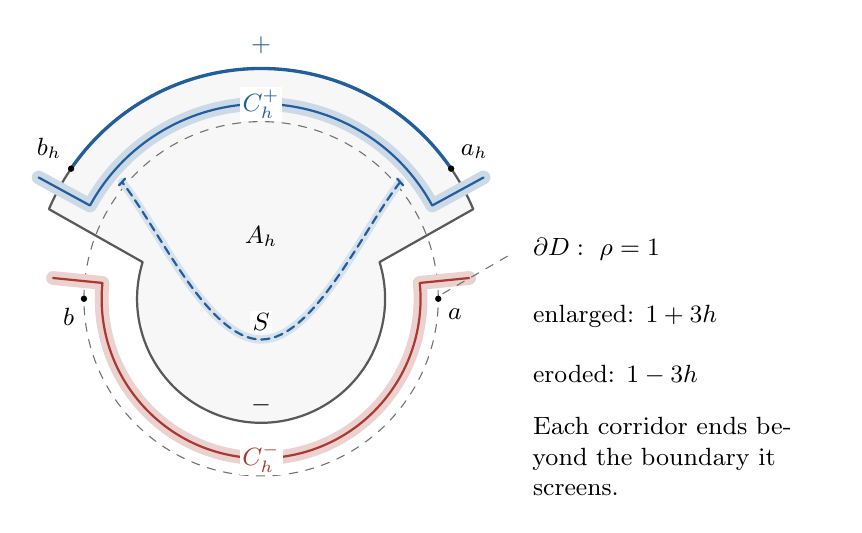
\begin{tikzpicture}[scale=2.25,line cap=round,line join=round,
  every node/.style={font=\small}]
 \definecolor{curveplus}{RGB}{35,94,156}
 \definecolor{curveminus}{RGB}{170,57,47}
 \fill[black!3]
   (17.2:.70)--(22.9:1.30) arc[start angle=22.9,end angle=157.1,radius=1.30]
   --(162.8:.70) arc[start angle=162.8,end angle=377.2,radius=.70]--cycle;
 \draw[black!65,thick]
   (17.2:.70)--(22.9:1.30) arc[start angle=22.9,end angle=157.1,radius=1.30]
   --(162.8:.70) arc[start angle=162.8,end angle=377.2,radius=.70];
 \draw[curveplus,very thick]
   (34.4:1.30) arc[start angle=34.4,end angle=145.6,radius=1.30];
 \draw[dashed,black!55] (0,0) circle[radius=1];
 \draw[curveminus!23,line width=5pt]
   (174.3:1.18)--(174.3:.90)
   arc[start angle=174.3,end angle=365.7,radius=.90]--(5.7:1.18);
 \draw[curveminus,thick]
   (174.3:1.18)--(174.3:.90)
   arc[start angle=174.3,end angle=365.7,radius=.90]--(5.7:1.18);
 \draw[curveplus!23,line width=5pt]
   (28.6:1.43)--(28.6:1.10)
   arc[start angle=28.6,end angle=151.4,radius=1.10]--(151.4:1.43);
 \draw[curveplus,thick]
   (28.6:1.43)--(28.6:1.10)
   arc[start angle=28.6,end angle=151.4,radius=1.10]--(151.4:1.43);
 \draw[curveplus!18,line width=3pt]
   (40:1.025) .. controls (.58,.40) and (.30,-.23) .. (0,-.23)
   .. controls (-.30,-.23) and (-.58,.40) .. (140:1.025);
 \draw[curveplus,densely dashed,thick]
   (40:1.025) .. controls (.58,.40) and (.30,-.23) .. (0,-.23)
   .. controls (-.30,-.23) and (-.58,.40) .. (140:1.025);
 \draw[curveplus,thick] (.768,.678)--(.802,.640);
 \draw[curveplus,thick] (-.768,.678)--(-.802,.640);
 \node[fill=white,inner sep=1pt] at (0,-.13) {$S$};
 \fill (0:1) circle[radius=.018] node[below right] {$a$};
 \fill (180:1) circle[radius=.018] node[below left] {$b$};
 \fill (34.4:1.30) circle[radius=.018] node[above right] {$a_h$};
 \fill (145.6:1.30) circle[radius=.018] node[above left] {$b_h$};
 \node at (0,.35) {$A_h$};
 \node[curveplus,fill=white,inner sep=1pt] at (0,1.10) {$C_h^+$};
 \node[curveminus,fill=white,inner sep=1pt] at (0,-.90) {$C_h^-$};
 \node at (0,-.60) {$-$};
 \node[curveplus] at (0,1.43) {$+$};
 \node[anchor=west] at (1.48,.28) {$\partial D:\ \rho=1$};
 \draw[dashed,black!55] (1.39,.24)--(1.01,.02);
 \node[anchor=west] at (1.48,-.10) {enlarged: $1+3h$};
 \node[anchor=west] at (1.48,-.43) {eroded: $1-3h$};
 \node[anchor=west,align=left,text width=3.7cm] at (1.48,-.89)
   {Each corridor ends beyond the boundary it screens.};
\end{tikzpicture}

 \caption{The minus-favoring construction for a small displacement $h>0$,
 in Schoenflies coordinates. Here $A_h$ is a sufficiently close polygonal
 approximation, in the physical plane, of the preliminary displaced
 topological domain; $a_h,b_h$ are its incoming and outgoing boundary marks.
 The dashed circle is $\partial D$. The preliminary boundary is enlarged
 along its middle plus arc and eroded elsewhere. The red minus corridor
 $C_h^-$ is outside $A_h$, including its caps; the blue plus corridor
 $C_h^+$ is outside $D$, and crosses the minus boundary of $A_h$ before
 its end gates. Corridor widths and radial displacements are exaggerated.
 The dashed blue strip $S$ illustrates an allowed plus strip: its gates
 lie just outside $D$, and the strip lies inside $A_h$, on the center
 side of both corridors.  Such strips are selected from a finite
 deterministic list before coupling any crossing events.  The diagram
 specifies topology and signs, not a metric distortion estimate for
 $\Psi$.}
 \label{fig:boundary-squeeze}
\end{figure}

Replace the boundary, corridors, scopes, and gates by sufficiently close
polygonal approximations in the physical plane.  One way to do this is
to subdivide each of the finitely many simple arcs into pieces lying in
disjoint small neighborhoods of nonadjacent pieces, then join points in
successive neighborhoods by polygonal arcs; small transverse polygonal
gates give the rectangles. The rectangular neighborhoods of the arcs
are transported from the coordinate plane by $\Psi$. Working within
these neighborhoods preserves the order and sides in the polygonal
approximations.  All the displayed disjointness conditions, cap
crossings, and gaps between designated arcs are open conditions with
positive clearance.  Hence they survive sufficiently close
approximations.  Denote the resulting polygonal domain by $A_h$ and its
marked points by $a_h,b_h$.  Choose the approximation errors tending to
zero with $h$, including in boundary parametrization.  Ordinary lattice
approximations of this fixed polygonal marked domain will always be used
for its pure Dobrushin law.

For the comparison favoring plus use the radial function
$R_h(\theta-\pi)$ instead.  Its incoming and outgoing marks have angles
$2\pi-6h$ and $\pi+6h$, respectively; the enlarged intervening arc
through $3\pi/2$ is minus, and its complement is plus.  Rotate the two
corridor placements by $\pi$ and interchange their colors.  Thus the
inner plus corridor lies outside this comparison domain and the outer
minus corridor lies outside $D$.  Orient its pure chord from the mark
near $a$ to the mark near $b$, as before.

We spell out why these are valid comparisons for the given target
approximations.  If $c$ parametrizes $\partial D$, then $\phi_n\circ c$
parametrizes $\partial D_n$ and converges uniformly to $c$.  On any compact
set disjoint from $\partial D$, winding numbers of these curves agree
eventually; thus membership in $D_n$ agrees there with membership in $D$.
On a closed subarc separated from $a,b$, the order along the boundary is
also preserved, since $\phi_n$ is a homeomorphism taking the two marks to
the prescribed marks.  Consequently every fixed clearance, inclusion,
and signed-arc placement above holds for $D_n$ for all sufficiently large
$n$.  Fine teeth or fjords lie in the shrinking boundary collar.  They do
not replace any actual exterior pin, and they do not intersect a compact
clearance chosen at fixed $h$.

An allowed \emph{plus strip} is a polygonal topological rectangle $S$
with two end gates, whose closure is in $A_h$, on the center side of both
cutting corridors and outside both reveal scopes.  Its two gates are
outside $\overline D$, on the enlarged plus portion.  We may require
$S\subset\Psi(\{\rho<1+h/2\})$, with a slight decrease of this bound
to absorb polygonal tolerances.  Wherever $S$ crosses $\partial D$, it
does so on $I_+$ with positive clearance from the marks.  Only strips
satisfying all these conditions are used.  The relevant portion of $A_h$
is on the center side of $C_h^-$ because that entire corridor is outside
$A_h$.  The strips needed below exist around compact subarcs of a pure
interface; their selection will be justified separately.

\begin{proposition}[Fixed-geometry boundary squeeze]
\label{prop:boundary-squeeze}
Fix the domain, signs, a displacement $h$, the preceding polygonal
placements, and a finite list $S_1,\ldots,S_m$ of allowed plus strips.
Let $V_A\in\{0,1\}^m$ record their plus crossings in the pure Dobrushin
law in an ordinary mesh approximation of $A_h$.  Let $V_n^+$ record plus
crossings in the target, filling the portions of the strips outside
$D_n$ virtually with plus.  There is a coupling with
\begin{equation}
 \P(V_A\leq V_n^+)=1-o(1) \qquad(n\longrightarrow\infty),
 \label{eq:curves-vector-order}
\end{equation}
where the inequality holds coordinatewise.  The error is uniform over
all admissible target exterior configurations.  The sign-reversed
construction gives the corresponding transfer of minus crossings from
pure domains favoring plus.  The smallness condition on $\lambda$ is the
one fixed at the beginning of the section; only the mesh threshold and
the error bound depend on these fixed geometries.
\end{proposition}

\begin{proof}
Place all sets in a torus chart with a fixed positive external buffer.
Let $E_h$ be the event of simultaneous lengthwise minus and plus
crossings of $C_h^-$ and $C_h^+$.  Proposition~\ref{prop:pure-rsw} gives
$\mu_{0,N}(E_h)\geq q_h>0$ for small mesh.  By
Theorem~\ref{thm:bulk-stability}, $\mu_{\lambda,N}(E_h)\geq q_h/2$
eventually, and the joint laws of
\[
 \bigl(\one_{E_h},V(S_1),\ldots,V(S_m)\bigr)
\]
in the pure and perturbed tori have total variation distance
$\varepsilon_n\to0$.  Here each $V(S_i)$ is an ordinary bulk crossing
test in the torus, without virtual filling.  For any two laws $p,q$ on
a finite space, an event $E$ with $p(E),q(E)\geq q_*>0$, and a random
vector $V$ on that space, subtraction of the two conditional fractions
gives
\begin{equation}
 \bigl\|p(V\in\cdot\mid E)-q(V\in\cdot\mid E)\bigr\|_{\TV}
 \leq \frac{2\|p-q\|_{\TV}}{q_*}.
 \label{eq:curves-conditioned-tv}
\end{equation}
Thus the two middle vectors conditioned on $E_h$ can be coupled to agree
with probability $1-o(1)$.  The laws $p,q$ in this application are the
joint indicator laws just displayed; no total variation estimate on the
underlying spin fields is used.

In each conditioned torus reveal the crossing closest to the radially
exterior side of each corridor.  Use the stopped reveal of
Lemma~\ref{lem:comparison-stopped-reveal}.  The transcript examines the
exterior side up to the crossing and leaves only pins of its prescribed
color facing the center.  The crossing and the event of its being the
first such crossing are determined by this transcript.  After both
transcripts have been conditioned upon, no additional crossing-existence
condition remains on the unrevealed center.  The two scopes are disjoint,
so the second reveal does not enter the core left by the first.

For precision, the free comparison components and all their boundary
incidences are as follows.  In the first comparison, the lower law is the
pure law in $A_h$, and the upper law is the conditioned pure torus.  Take
the components of the common free region on the center side of its
revealed plus path.  This path is an upper plus pin against lower free
spins.  All accessible portions of $\partial A_h$ are lower minus pins
against upper free spins: the plus boundary is screened by the revealed
path, whose caps continue outside $A_h$.  At a meeting of a path and a
boundary, the pair is upper plus against lower minus.  The minus reveal
is outside $A_h$ by~\eqref{eq:curves-scope-clearances}.  These checks give
a joint comparison on all spins used by the strips, and therefore
\[
 V_A\leq V_0^{E_h}.
\]

In the second comparison the lower law is the conditioned perturbed
torus and the upper law is the target.  Take the common free components
on the center side of the revealed minus path.  On this path the lower
pin is minus and the upper vertex is free.  The target minus arc is
screened by this path and its caps.  Every remaining accessible target
boundary neighbor is an upper plus pin against a lower free vertex.
Where the two cuts meet, the pair is upper plus against lower minus.
The plus reveal lies outside the target.  The comparisons are precisely
\[
 (\text{upper},\text{lower})=(+,\text{free}),\quad
 (\text{free},-),\quad (+,-).
\]
No same-sign pinned pair, and no monotonicity of an arbitrary pinned
perturbed factor, is being assumed.  A diagonal segment of a separating
triangulated path cannot be crossed by the interior of a nearest-neighbor
edge.  Thus each nearest-neighbor incidence leaving a comparison
component actually meets one of the path or arc pins just enumerated.
This remains true when a strip exits and reenters $D_n$.  Condition on
all other auxiliary bits as in Proposition~\ref{prop:strict-incidence};
the strict inequalities are uniform in those bits and hence in the
unprescribed spin pattern farther behind the arcs.  The resulting spin
comparison and the extremal virtual values outside $D_n$ give
\[
 V_\lambda^{E_h}\leq V_n^+.
\]

Finally glue the two order couplings with the equality coupling supplied
by~\eqref{eq:curves-conditioned-tv}.  This is elementary disintegration
on finite spaces: first sample each common middle vector, then sample
the remaining variables from the relevant conditional laws.  Extend the
outer vectors to their complete configurations in the same way.  This
proves~\eqref{eq:curves-vector-order}.  In particular the conclusion is
about a finite vector of tests, not a total variation comparison of spin
configurations.  Interchanging plus and minus and exchanging the
enlarged and eroded arcs proves the other assertion.
\end{proof}

The virtual filling in the proposition is a rule for evaluating a spin
crossing.  We now justify its use as a geometric barrier, including at
corners of the target boundary.

\begin{lemma}[Local drawing beside a signed strip]
\label{lem:curves-local-barrier}
Fix finitely many allowed plus strips and, in the sign-reversed
construction, finitely many allowed minus strips.  For all sufficiently
large $n$, the prescribed target curve has a drawing $\widetilde\gamma_n$
with the same traversal order and
\[
 d_{\rm curv}(\widetilde\gamma_n,\gamma_n)=O(\delta_n)
\]
that is disjoint from every monochromatic crossing of its respective
virtually filled strip.  The two half-stubs and neighborhoods of the
marks can retain their original drawings.  The filling and redrawing
change no spin in the conditional law and remove no interaction term.
\end{lemma}

\begin{proof}
Consider first a plus strip.  Its boundary contacts lie on a compact
subarc of $I_+$ separated from the marks.  For large $n$, the same is
true of its contacts with $\partial D_n$.  Every exterior vertex sharing
a nearest-neighbor bond with the domain at those contacts is already
plus, by Lemma~\ref{lem:contour-spin}.  Fill the remaining exterior
vertices of the incident square faces with plus for the purpose of
drawing only.

Inspect a square face of the primal lattice, or equivalently the four
cells incident to one dual vertex.  The Jordan condition allows one,
two adjacent, or three interior cells at a boundary vertex; two opposite
interior cells alone would give a diagonal pinch.  With one interior
cell, its two nearest exterior neighbors are already plus.  Only the
opposite exterior vertex might have a different actual spin, and filling
it leaves every disagreement edge in $E_{\Omega_n}$ unchanged.  The
resulting zero set joins the two occupied domain edges when there are
two.  With two adjacent or three interior cells, every exterior cell
of the face is a nearest exterior neighbor, so its spin already has the
filling value.  In each case the interpolated zero segments have exactly
the partial contour's connections: its unique connection at degree two,
and the prescribed NE/SW pairing at degree four.  Faces wholly inside
the domain have the same property without filling.

Redraw the target portions in all faces meeting the strip, together
with one adjacent lattice layer, as the corresponding zero segments.
A monochromatic edge of the triangulation is disjoint from that zero
set.  Both the original drawing and each replacement meet a face side
at the same disagreement-edge midpoint.  The replacements therefore
glue to one another and to the unchanged portions without changing a
local connection.  Matching the successive face crossings in their
original order gives the displayed $O(\delta_n)$ curve distance.

The minus construction is identical with the colors exchanged.  The
boundary-contact sets of the fixed plus and minus strip lists have
positive separation from each other and from the marks.  Therefore,
for sufficiently fine mesh, no face receives conflicting filling
instructions.  In the bulk both instructions use the actual spins.
The replacements can consequently be made simultaneously, leaving the
marked neighborhoods and half-stubs untouched.  This is a modification
of the drawing, not an interpolation of the actual full-plane exterior
configuration.  In particular all farther exterior spins and every
interaction across a narrow fjord remain in the Gibbs conditional law.
\end{proof}

\subsection{From fixed strip tests to limiting barriers}

We first record the domain-continuity fact needed for the displaced pure
curves.  If Jordan boundaries $c_j:\partial\mathbb D\to\partial G_j$
are homeomorphic parametrizations converging uniformly to a Jordan
parametrization $c$, normalized conformal maps
$f_j:\mathbb D\to G_j$ converge uniformly on $\overline{\mathbb D}$
to the corresponding map onto $G$.  Normalization can be by one fixed
interior point and positive derivative, or by three convergent distinct
boundary points.  Here is the reason the boundary assumption matters.
Uniform convergence to the injective $c$ implies a uniform local
connectedness modulus for the boundaries: nearby endpoints have one
boundary subarc of small diameter.  Indeed, otherwise inverse
uniform continuity of $c$ and uniform continuity of the parametrizations
would give two separated parameter arcs with arbitrarily close images.
Kernel convergence gives local uniform convergence of the normalized
maps.  The boundary crosscut proof of the Carath\'eodory extension
theorem, applied with this common local connectedness modulus, gives
equicontinuity on the closed disk, and hence upgrades local convergence
to uniform convergence.  This is Rad\'o's Jordan-domain continuity
theorem \citep[Th\'eor\`eme, p.~182]{Rado1923}.  Its stated uniform
convergence is on the closed disk.  It requires more than kernel
convergence alone.

For clarity, the crosscut argument is uniform here.  The image areas are
bounded by a common containing disk.  Cauchy--Schwarz on circular arcs
centered at a boundary point of $\mathbb D$, followed by integration in
their radii, supplies a crosscut of image length tending to zero between
any two sufficiently small separated radius scales; the squared length
bound is a constant divided by the logarithm of their ratio.  Its image
endpoints are close.  The common local connectedness modulus bounds the
diameter of the smaller boundary subarc joining them.  The image
crosscut together with that subarc cuts off a set of comparably small
diameter.  The component not containing the fixed normalized interior
point is this small component, since that point has fixed positive
distance from the boundary.  This controls the images of the smaller
boundary neighborhood uniformly.  Finite covering of the unit circle
then proves the required equicontinuity.  Boundary normalization follows
by precomposing with disk automorphisms; the preimages of the three
distinct limiting marks converge by injectivity of the limiting boundary
map.

To account explicitly for the moving marks, first normalize $f_h,f$ by
a common interior point and positive derivative.  If $\alpha_h,\beta_h$
are the boundary preimages of $a_h,b_h$, uniform convergence on the
closed disk and injectivity of $f$ imply
$\alpha_h\to\alpha=f^{-1}(a)$ and
$\beta_h\to\beta=f^{-1}(b)$.  Fix a third boundary point different
from $\alpha,\beta$.  The disk automorphism taking
$\alpha,\beta$ to $\alpha_h,\beta_h$ and fixing that third point
converges uniformly on the closed disk to the identity.  Precomposition
by these automorphisms therefore gives uniformly convergent maps with
the required marked endpoints.

Applying this fact to $A_h$, and coupling by a single disk $\SLE_3$,
shows that its continuum pure interface law converges as $h\downarrow0$
to chordal $\SLE_3$ in $D$ from $a$ to $b$, in the oriented uniform curve
metric.  The same holds for the plus-favoring comparison domains.  This
uses the conformal definition of $\SLE_3$ and its continuous simple trace;
uniform convergence of the conformal maps bounds the distance between
the corresponding image curves.  For fixed $h$ the lattice convergence
used here is only Theorem~\ref{thm:pure-sle} in an ordinary polygonal
approximation of $A_h$.

\paragraph{Choosing a deterministic finite list.}
Couple
the continuum curves in $A_h$ to their limit $\Gamma$ so that their
oriented distances tend to zero.  The curve $\Gamma$ meets $\partial D$
only at $a,b$.  For every fixed small parameter interval removed from
each end, its remaining compact subarc is a positive distance inside
$D$.  Uniform convergence implies that, with probability tending to one
as $h\downarrow0$, a middle subarc of the curve in $A_h$ lies below
$\rho=1+h/2$, has endpoints outside $\overline D$, and the omitted
terminal pieces have diameter tending to zero.  To make this choice
without a regularity assumption on level hits, choose a point of the
curve deep inside $D$, take the last hit of $\rho=1+h/3$ before that
point and the first hit after it.  The intervening subarc lies in
$\rho\leq1+h/3$.  Both hits lie outside $D$ on the enlarged plus arc.
Extend this subarc slightly at its two ends, within
$\rho<1+h/2$, before choosing gates.  Compact parts away from $a,b$
cannot contain these hits in the limit.  The omitted portions therefore
shrink in diameter.  Polygonal tolerances can be chosen smaller than the
gaps between these levels.

For each such simple subarc, a rectangular neighborhood of a slightly
extended arc gives a thin strip with transverse end gates lying outside
$D$.  Polygonal approximation of its sides and gates gives an allowed
strip.  One can prescribe a continuous parametrization of its
cross-sections such that each section has small diameter and stays near
the corresponding point of a simple polygonal prototype.  A lengthwise
traversal then stays near this prototype, even if it backtracks.  The
extended subarc crosses both gates with a margin, and stays away from
the long sides.  These properties persist in an open neighborhood in
the oriented curve metric.  On sufficiently fine lattices, a traversal
by the pure interface with these margins supplies a plus spin crossing
of the strip: follow its plus side in the fixed triangulation and crop
at the gates.  The discrepancy between that side and the interface is
$O(\delta_n)$, smaller than the fixed margin.

The strip construction can be made from a countable collection, using
rational polygonal vertices and rational positive margins.  These open
curve neighborhoods cover all the favorable continuum curves just
described.  The curve space is separable; equivalently use this explicit
countable collection and continuity from below of probability.  A finite
subcollection thus covers all but any prescribed positive probability.
Fix that entire finite list before using
Proposition~\ref{prop:boundary-squeeze}.  After its joint vector coupling
has been made, the pure curve may select one strip from the list.  The
corresponding target crossing then exists outside an event of vanishing
probability.  No test chosen adaptively from an infinite family has
been inserted into Theorem~\ref{thm:bulk-stability}.

\paragraph{Passing to moving geometries.}
Choose errors
$\epsilon_j\downarrow0$.  First choose $h_j\downarrow0$, polygonal
comparison domains of both signs, and favorable continuum events whose
omitted end pieces have diameter at most $\epsilon_j$, with failure
probability at most $\epsilon_j$.  Then choose finite strip covers with
widths and prototype errors at most $\epsilon_j$ and additional failure
probability at most $\epsilon_j$.  Finally choose increasing integers
$n_j$ so that for every $n\geq n_j$ the fixed placements, both pure
interface approximations, and both finite-vector couplings have all
their required errors at most $\epsilon_j$.  Set
\begin{equation}
 j(n)=\max\{j\leq n:n_j\leq n\},
 \label{eq:curves-slow-diagonal}
\end{equation}
with an arbitrary definition before $n_1$.  This index tends to infinity.
The constants $q_{h_j}$ in~\eqref{eq:curves-conditioned-tv} may tend to
zero; the threshold $n_j$ has already absorbed their reciprocals.
Couple each of the two comparison constructions with the target and
glue over the target configuration.  Their comparison curves need not
be independent.  Both marginal laws converge to the same chordal
$\SLE_3$ law, and, with probability tending to one, the target has both
colored barriers in strips converging to those comparison curves.

\subsection{Forbidden sides, order, and identification of the trace}

For a simple chord $C$ of $D$ from $a$ to $b$, with interior in $D$, let
$P(C)$ and $M(C)$ be the open components of $D\setminus C$ adjacent to
$I_+$ and $I_-$, respectively.  Their closures below are in $\overline D$.
All target traces lie in one fixed compact set for large $n$.  The space
of nonempty compact subsets of that set is compact in Hausdorff distance.
Consequently, along any mesh subsequence we can pass further to a joint
limit
\[
 (\operatorname{tr}\gamma_n,L_n,U_n)\ \Longrightarrow\ (K,L,U),
\]
where $L_n,U_n$ are the two comparison curves in the slow diagonal.
Their marginal curve laws are tight by the preceding construction.
The limit $K$ is connected and contains $a,b$: separation of a compact
limit into two sets at positive distance would separate every
sufficiently close connected approximant.  Also $K\subset\overline D$:
winding stability excludes every fixed compact set outside
$\overline D$ from $D_n$ eventually, and the drawing displacements
vanish.  The curves $L,U$ have the
chordal $\SLE_3$ marginal law.  Use a representation of this joint
convergence in which the compact and curve distances tend to zero
almost surely, and pass to a further subsequence so that barrier failures
also occur only finitely often.

We claim that the barriers imply
\begin{equation}
 K\subset\overline{M(L)}\cap\overline{P(U)}.
 \label{eq:curves-forbidden-sides}
\end{equation}
Choose once and for all $\rho_*>1$, independently of $h$ and $n$, and
restrict to $h$ with $1+h/2<\rho_*$.  Consider the plus barrier associated
with $L_n$.  Erase loops from a successful strip crossing and connect its
ends to the gate centers within exterior gate neighborhoods.  In
Schoenflies coordinates, close this path by radial segments from the gate
centers to $\rho=\rho_*$ and the plus-side circular arc between them.
For each fixed $h$ these added paths have positive clearance from
$\overline D$, so they lie outside $D_n$ for all sufficiently large $n$;
include this requirement in the choice of $n_j$.  Together these paths
form a closed barrier disjoint from the redrawn target
$\widetilde\gamma_n$ of Lemma~\ref{lem:curves-local-barrier}.  We use
this exact disjointness here; $O(\delta_n)$ closeness alone would not
preserve disjointness from a lattice barrier.  Both target marks are on
its zero-winding exterior side: their outward escape paths
lie beyond the ends of the extended plus arc and avoid the strip, whose
ends are inside the target plus arc and separated from the marks.  Thus
the entire redrawn target interface has zero winding relative to the
closed barrier.

On every compact subset of $P(L)$, the barrier has, for large $n$, the
same nonzero winding as $L$ closed around $I_+$ outside $D$.  To verify
this without controlling the traversal order of the target crossing,
use the rectangular chart of the strip.  Any path connecting its two end
gates is homotopic, relative to those gates, to its central prototype;
its loops can be removed inside the strip.  Its winding about a point
outside that strip is therefore the prototype's winding.  The widths
vanish, the prototypes converge in curve distance to $L$, and the
terminal errors shrink to $a,b$.  The gate centers therefore tend to
$a,b$, and their radial connectors tend to the endpoint radial segments.
On every compact subarc of $I_+$, the fixed-radius part of the closure
stays a positive distance beyond $\partial D$, while the connectors
remain away from that subarc.  The same winding conclusion consequently
holds on small neighborhoods of every point of $I_+$ other than $a,b$.
The redrawn target cannot enter these neighborhoods.  Its trace has
the same Hausdorff limit $K$ as the original target, by
Lemma~\ref{lem:curves-local-barrier}.  This excludes both $P(L)$ and
the open plus boundary arc from $K$, leaving
$K\subset\overline{M(L)}$.  The minus barrier proves
$K\subset\overline{P(U)}$.  The half-stubs remain near the marks and
therefore do not meet these fixed neighborhoods.

\begin{lemma}[Ordered chords with equal laws]
\label{lem:ordered-chords}
Let $L,U$ be random simple chords from $a$ to $b$ in a Jordan domain,
meeting its boundary only at their endpoints, and let $K$ be a random
compact connected subset of its closure containing $a,b$.  Suppose
\eqref{eq:curves-forbidden-sides} holds almost surely.  Then
$P(L)\subset P(U)$ almost surely.  If $L$ and $U$ have the same trace
law, then $L=U=K$ as compact sets almost surely.
\end{lemma}

\begin{proof}
Work in the closed disk using a fixed Schoenflies map.  If
$P(L)\cap M(U)$ were nonempty, connect a point of that intersection to
an interior point of $I_+$ through $P(L)$ and to an interior point of
$I_-$ through $M(U)$.  The two side domains are Jordan domains.  Small
endpoint arcs and interior polygonal paths, with loops removed, therefore
give a simple crosscut between these opposite boundary arcs, contained
in their union except for its two boundary endpoints.  This crosscut is
disjoint from $K$ by~\eqref{eq:curves-forbidden-sides}.  Its endpoints
alternate with $a,b$ around the circle, so it separates $a$ from $b$ in
the closed disk.  This contradicts connectedness of $K$.  Hence
$P(L)\cap M(U)=\varnothing$.  It follows that
$P(L)\subset P(U)\cup U$.  No interior point of $U$ can lie in the open
set $P(L)$: every neighborhood of such a point meets $M(U)$.  Thus
$P(L)\subset P(U)$.

Let $X,Y$ be the ordinary planar areas of the two plus sides after this
fixed disk map.  They are bounded random variables, $X\leq Y$, and their
distributions agree when the trace laws agree.  Thus $\E(Y-X)=0$ and
$X=Y$ almost surely.  Proper inclusion of these particular side domains
would give strictly different areas.  Indeed a point of
$P(U)\setminus P(L)$ either belongs to $M(L)$, or lies on $L$; in the
latter case its open neighborhood in $P(U)$ meets $M(L)$.  In either
case the difference contains a nonempty open subset of $M(L)$, of
positive area.  Consequently $P(L)=P(U)$ and their interior boundaries
give the same chord.  This reasoning does not require the chords to
have zero area.  Finally~\eqref{eq:curves-forbidden-sides} puts $K$
inside that chord.  The inverse of a simple parametrization sends $K$
to a connected subset of $[0,1]$ containing both endpoints, which is all
of $[0,1]$.
\end{proof}

The lemma identifies every subsequential target trace limit as chordal
$\SLE_3$.  We have also excluded a boundary segment from that trace.
We have not yet excluded repeated forward and backward travel in a
thin neighborhood of the same chord.  The next argument supplies that
last distinction.

\subsection{Interior passages and the orientation of the limit}

For a compact $F\Subset D$ and a fixed $R>0$ small enough that all
radius-$2R$ neighborhoods of $F$ lie in $D$, let $\mathcal B_n(F;r,R)$
be the event that the target contour has at least four passages across
an annulus with some center in $F$, inner radius $r$, and outer radius
$R$.  Passages count disjoint parameter intervals, with endpoint hits
allowed to coincide, as in Section~\ref{sec:stability}.  Square or round
annuli can be used, after fixed-factor changes of radii.  We claim
\begin{equation}
 \lim_{r\downarrow0}\limsup_{n\to\infty}
 \P\bigl(\mathcal B_n(F;r,R)\bigr)=0.
 \label{eq:curves-uniform-bottleneck}
\end{equation}
Cover the fixed $2R$-neighborhood by finitely many interior boxes with
fixed positive free buffers.  Proposition~\ref{prop:interior-density}
compares each of their target spin marginals pointwise with a torus
marginal, with a constant independent of $r,n,\tau_n$.  A grid of mesh
comparable to $r$ has $O_F(r^{-2})$ centers.  Four target passages about
any center in $F$ give four passages about a nearest grid center from
radius $Cr$ to radius $R/C$, by cropping the same paths at their hits.
At each grid center enlarge this to the event $F_4$ that \emph{any}
locally resolved contours supply four passages through that annulus.
This enlarged event is determined by the spins in the annulus and a
one-face margin.  Identifying the marked target component is not local,
but is unnecessary for this upper bound.  The bulk drawing comparison
absorbs its $O(\delta_n)$ displacement into the fixed radius crops.

For each fixed $r$ the enlarged events are finitely many fixed bulk
tests of Section~\ref{sec:stability}, and the density comparison applies
to them.  Theorem~\ref{thm:bulk-stability} and
Proposition~\ref{prop:pure-four-passages} bound their torus mesh upper
limits by $C_R(r/R)^{2+c}$ for some $c>0$ when $r/R$ is small.  A union
bound and the fixed density constants give an upper bound $C_{F,R}r^c$
after the mesh limit.  This proves~\eqref{eq:curves-uniform-bottleneck}.
The buffer in the density comparison was fixed before $r$ decreased;
there is no density constant at a shrinking buffer hidden in this bound.
The finite grid union also gives a measurable upper event for arbitrary
centers, so no measurable choice of a center is required below.

\begin{lemma}[Progress coordinates and the full curve metric]
\label{lem:curve-upgrade}
Let $\Gamma:[0,1]\to\overline D$ be continuous and injective, with
$\Gamma(0)=a$, $\Gamma(1)=b$, and $\Gamma((0,1))\subset D$.  Let
$g_n:[0,1]\to\C$ be continuous simple curves whose endpoints tend to
$a,b$ and whose traces tend in Hausdorff distance to $\Gamma([0,1])$.
There are continuous functions $u_n:[0,1]\to[0,1]$ with endpoint
values tending to $0,1$ such that
\begin{equation}
 e_n:=\sup_t|g_n(t)-\Gamma(u_n(t))|\longrightarrow0.
 \label{eq:curves-coordinate-error}
\end{equation}
Put $B_n=\sup_{s<t}(u_n(s)-u_n(t))$.  If $B_n\to0$, then
$d_{\rm curv}(g_n,\Gamma)\to0$.  Conversely, for every fixed $0<\eta<1$, a backward
drop $B_n\geq\eta$, with $n$ sufficiently large, forces six disjoint
passages from radius $r$ to one fixed radius $R_\eta>0$, for every
$e_n<r<R_\eta$, about a center on
$\Gamma([\eta/2,1-\eta/2])\Subset D$.

For random curves, suppose the trace and endpoint convergence hold in
probability in a coupling with such a random $\Gamma$, and suppose
\eqref{eq:curves-uniform-bottleneck} holds for every deterministic
compact interior $F$ and sufficiently small fixed $R$.  Then
$d_{\rm curv}(g_n,\Gamma)\to0$ in probability in that coupling.
\end{lemma}

\begin{proof}
The inverse coordinate $\Gamma^{-1}$ is continuous on the compact
trace.  Extend it continuously, with values in $[0,1]$, to a compact
ambient neighborhood and call the extension $p$.  Setting
$u_n=p\circ g_n$ gives~\eqref{eq:curves-coordinate-error} by uniform
continuity: a point close to $\Gamma(v)$ has $p$-value close to $v$,
and hence is close to $\Gamma(p(\cdot))$.  The endpoints have the
asserted coordinates.

Here is the matching when drops vanish.  The running maximum
\[
 m_n(t)=\max_{s\leq t}u_n(s)
\]
is continuous, nondecreasing, and satisfies
$0\leq m_n(t)-u_n(t)\leq B_n$.  Its endpoint values tend to $0,1$.
For all large $n$ let
\[
 v_n(t)=\frac{m_n(t)-m_n(0)}{m_n(1)-m_n(0)},\qquad
 h_n(t)=(1-\kappa_n)v_n(t)+\kappa_n t,
\]
where $0<\kappa_n\downarrow0$.  Then $h_n$ is an increasing
homeomorphism of $[0,1]$ and $\|h_n-u_n\|_\infty\to0$.  If
$\omega_\Gamma$ denotes the modulus of continuity of $\Gamma$, then
\[
 d_{\rm curv}(g_n,\Gamma)
 \leq e_n+\omega_\Gamma(\|h_n-u_n\|_\infty)\longrightarrow0.
\]
This uses exactly the allowed matching in~\eqref{eq:curve-metric},
with the identity on $g_n$ and $h_n$ on $\Gamma$.

For the converse, the continuous function $u_n(s)-u_n(t)$ attains its
maximum on $0\leq s\leq t\leq1$.  If $B_n\geq\eta>0$, a maximizing
pair has $s<t$ and $u_n(s)-u_n(t)\geq\eta$.  Set
$c_n=(u_n(s)+u_n(t))/2\in[\eta/2,1-\eta/2]$.  When the endpoint
coordinate errors are less than $\eta/4$, each of the intervals
$[0,s]$, $[s,t]$, and $[t,1]$ has endpoints on opposite sides of
$c_n$, at coordinate distance at least $\eta/4$.  Each therefore
contains a visit to $c_n$.  Injectivity and compactness imply
\[
 q_\eta=\min_{|v-w|\geq\eta/4}|\Gamma(v)-\Gamma(w)|>0,
 \qquad
 d_\eta=\dist(\Gamma([\eta/2,1-\eta/2]),\partial D)>0.
\]
Choose $R_\eta<\min(q_\eta,d_\eta)/4$.  Once $e_n<R_\eta$, the
four anchor points $g_n(0),g_n(s),g_n(t),g_n(1)$ are outside the
radius-$R_\eta$ disk about $\Gamma(c_n)$, whereas each of the three
level visits is within $e_n$ of its center.  In each time interval crop
the incoming and outgoing portions at the last outer and first inner
hits, and at the last inner and first outer hits.  For every
$e_n<r<R_\eta$ this supplies two annular passages.  The six parameter
interiors are disjoint, and simplicity gives disjoint spatial interiors.
They are thus six passages in the stated convention, and in particular
at least four.  Fixed-factor cropping gives the same assertion for
square annuli.

We give the measurability and order of limits for a random $\Gamma$.
Take a measurable continuous representative, for example the image of
a disk SLE representative in the coupling above.  We need not choose
a random extension $p$.  Write
$\Delta_n=d_H(\operatorname{tr}g_n,\operatorname{tr}\Gamma)$,
$z_n=2\Delta_n+1/n$, and define instead
\begin{equation}
 u_n(t)=
 \frac{\int_0^1 v\,(z_n-|g_n(t)-\Gamma(v)|)_+\,dv}
      {\int_0^1 (z_n-|g_n(t)-\Gamma(v)|)_+\,dv}.
 \label{eq:curves-measurable-coordinate}
\end{equation}
The denominator is positive since every $g_n(t)$ is within $\Delta_n$
of the trace, and continuity gives a parameter interval with positive
weight.  This coordinate is continuous in $t$ and jointly measurable.
Let
\[
 \iota_\Gamma(r)=\sup\{|v-w|:|\Gamma(v)-\Gamma(w)|\leq r\}.
\]
It tends to zero as $r\downarrow0$.  All parameters receiving positive
weight in~\eqref{eq:curves-measurable-coordinate} have diameter at most
$\iota_\Gamma(2z_n)$, and their weighted average lies between their
extreme values.  Consequently
\[
 e_n\leq z_n+
 \omega_\Gamma(\iota_\Gamma(2z_n))\longrightarrow0
\]
in probability; the endpoint coordinate errors also tend to zero.
These assertions follow first almost surely along any subsequence on
which $\Delta_n$ and the endpoint errors converge almost surely, and
hence hold in probability for the full sequence.

Fix $0<\eta<1$ and an exceptional probability $\zeta>0$.  Since
$q_\eta,d_\eta$ are strictly positive random variables, choose
deterministic $q,d>0$ such that
\[
 \P(q_\eta<q\ \text{or}\ d_\eta<d)<\zeta.
\]
The random centers then lie in the deterministic compact set
$F_d=\{z\in\overline D:\dist(z,\partial D)\geq d\}$, and one
deterministic $R<\min(q,d)/8$ works.  For each fixed $0<r<R$,
the preceding six-passage argument, outside an event of probability
$\zeta+o(1)$, bounds the probability of a drop of size $\eta$ by
$\P(\mathcal B_n(F_d;r,R))$.  First let $n\to\infty$, then
$r\downarrow0$ using~\eqref{eq:curves-uniform-bottleneck}, and finally
$\zeta\downarrow0$.  Thus $B_n\to0$ in probability.  To deduce curve
distance convergence, first choose a deterministic coordinate tolerance
on which $\omega_\Gamma$ is small outside probability $\zeta$, then use
the running-maximum bound and let $n\to\infty$.  Finally remove
$\zeta$.  This localizes the continuity modulus as well as the
injectivity and boundary-distance moduli.  All annulus radii and compact
charts are deterministic before the mesh limit is taken.
\end{proof}

The simplicity used in this lemma holds for the prescribed locally
resolved interface: the resolved embedded graph has degree two except
at its two degree-one stub midpoints, so its connecting component is an
embedded arc.  Distinct visits to a small disk along that arc count as
distinct passages.  No estimate for path length is required.  The lemma
also explains why a separate boundary passage estimate is unnecessary
at this stage: the limiting chord avoids the boundary away from its
endpoints, and its short terminal parameter intervals have arbitrarily
small diameter by continuity.

\subsection{Completion of the universality theorem}

\begin{proof}[Proof of Theorem~\ref{thm:main}]
For the fixed finite-range real potential $U$, Lemma~\ref{lem:contour-spin}
converts the exact contour weight into a finite-range, even,
square-symmetric spin perturbation, with all interactions meeting the
interior retained.  Theorem~\ref{thm:transfer} and
Theorem~\ref{thm:critical-trajectory} give an analytic bulk choice
$\beta_c(J,U,\lambda)$ near
$\beta_0=\log(1+\sqrt2)/(2J)$, positive for sufficiently small real
$\lambda$ of either sign and equal to $\beta_0$ at zero.  Shrink this
interval once to satisfy the independent-edit stability threshold and
the finite-table strict-incidence margins.  This gives a number
$\lambda_0(J,U)>0$ before any choice of $D,a,b$, approximation, exterior
contours, corridor, or strip.  The universal fixed-shape bootstrap in
Theorem~\ref{thm:bulk-stability} is what permits all later fixed
geometries to use this same interval.

Fix any $|\lambda|<\lambda_0$, any bounded Jordan marked domain, any
sequence of meshes and uniformly boundary-parametrized Jordan lattice
domains in the theorem, and any admissible sequence $P_{o,n}$.  On each
subsequence pass further so that the choice of plus boundary arc is
fixed.  The exact conditional-law reduction permits the target to be
placed in a buffered torus chart while retaining all its exterior pins.
Finite range permits any continuation beyond that chart without changing
the conditional law.  Proposition~\ref{prop:boundary-squeeze}, the
finite strip construction, and the slow diagonal produce a joint limit
of every further Hausdorff-convergent subsequence with two comparison
chords of the same $\SLE_3$ law.  Their forbidden-side inclusions and
Lemma~\ref{lem:ordered-chords} identify the target trace with that chord.
Thus the target traces converge in law in Hausdorff distance to chordal
$\SLE_3$.

Lift the subsequential trace coupling to the target paths using their
conditional distributions given their traces.  At each mesh the spin
space is finite, so this disintegration is immediate and preserves every
target passage probability.  No tightness of these path variables is
needed to perform the lift.  The limiting chord already has a measurable
continuous representative from its SLE marginal.  The interior density
comparison and bulk
four-passage estimate give~\eqref{eq:curves-uniform-bottleneck}, uniformly
in the permitted exterior configurations.  Lemma~\ref{lem:curve-upgrade}
therefore gives convergence in probability in the oriented curve metric
in this representation, and hence convergence in distribution in that
metric.  Since every subsequence has a further subsequence with this
same limit, the full sequence converges.  This argument also gives
tightness in the requested curve topology; it did not assume it for
the perturbed paths.

\widowpenalty=10000
The conclusion concerns the prescribed $\gamma_n$.  The local
redrawings used for its barriers preserve traversal order and have
$O(\delta_n)$ curve distance from it; they were used only to identify
its trace limit.  The half-stubs remained part of the original curve,
with endpoints tending to $a,b$, and the orientation is always from
the incoming midpoint to the outgoing midpoint.  The unit-lattice
potential $U$ was fixed throughout; only coordinates were multiplied by
$\delta_n$.  No sign
condition on $U$ or $\lambda$, boundary regularity beyond the stipulated
Jordan parametrizations, or restriction on the additional exterior
contours was imposed.  The value of $\beta_c$ and its interval of
validity are consequently independent of every domain and boundary
choice required in the theorem.
\end{proof}

The public mathematical results used in the argument are credited at their points of use.

\let\originalbibsection\bibsection
\renewcommand{\bibsection}{\originalbibsection\addcontentsline{toc}{section}{References}}
\begingroup
\raggedright
\bibliographystyle{plainnat}
\bibliography{references}
\endgroup
\end{document}
